%% This is an example first chapter.  You should put chapter/appendix that you
%% write into a separate file, and add a line \include{yourfilename} to
%% main.tex, where `yourfilename.tex' is the name of the chapter/appendix file.
%% You can process specific files by typing their names in at the 
%% \files=
%% prompt when you run the file main.tex through LaTeX.

\chapter{Experimentos y Resultados}
\label{eyr}

* Se van a hacer modelos de redes neuronales, redes bayesianas,
etc. con los datos (presentar los parámetros de estos modelos y qué
complicaciones tuvimos)
* Se van a extraer cuáles son las características más relevantes para
cada uno de los sentimientos, con el objetivo de lograr un kappa de
más de 0.21 y una precisión cercana al 60\%. (explicar cosas curiosas
sobre esto talvez)

\section{Experimentos}

Para los experimentos, se decidió usar clasificadores basados en redes
neuronales, Bayes ingenuo, k vecinos más cercanos, y árboles de
decisión. Todos los experimentos fueron realizados en RapidMiner.

En los casos explicados en esta sección y en la sección de Resultados,
la precisión significa el porcentaje de observaciones clasificadas
correctamente de acuerdo al dataset utilizado. El coeficiente de Kappa
significa qué tanto influyó el azar en las decisiones del
clasificador. Un Kappa de 0 significa que las decisiones fueron
completamente al azar, mientras que un Kappa de 1 significa que no
influyó en absoluto. De acuerdo a Landis y Koch
\cite{landis1977measurement}, un Kappa entre 0.21 y 0.4 es considerado
como suficiente. En estos experimentos se trata de conseguir un valor
en este intervalo. Conseguir valores más altos sería muy raro, debido
a que trabajar con dinámica de tecleo en textos libres (el usuario
tiene completa libertad sobre cuánto y qué escribir) es muy
difícil. Por lo general, precisiones del 60\% y coeficientes de Kappa
mayores a 0.21 es suficiente para considerar que los clasificadores
tuvieron éxito en estos casos.

Para las redes neuronales se siguió una arquitectura feedforward
y basada en backpropagation, con dos capas ocultas con 20 neuronas
cada una. La taza de aprendizaje fue de 0.6, y el momentum de
0.6. Para todas las ocasiones, las redes neuronales fueron entrenadas
por 200 generaciones. Un valor más apropiado hubiera sido un número de
generaciones mucho mayor (por ejemplo, 2000), pero el entrenamiento de
las redes neuronales tomó mucho tiempo aún con 200
generaciones. Además, como ha sio mencionado anteriormente, el
objetivo del entrenamiento de los clasificadores era meramente
encontrar un subconjunto de características que arrojara una precisión
cercana a 60\% y un Kappa de por lo menos 0.21. Con 200 generaciones
los clasificadores fueron capaces de encontrar un subconjunto que
reuniera todos los requisitos, a excepción del entrenamiento para el
estado emocional de Relajación; en este caso se obtuvo un Kappa de
0.207 (0.343 en promedio, con una desviación estándar de 0.136).

En el caso de los clasificadores basados en Bayes ingenuo, se
obtuvieron excelentes resultados en general. La mayoría
de las precisiones estuvieron arriba de 60\%, siendo la Concentración
y la Distracción las únicas excepciones. Los valores de Kappa fueron
todos por encima de 0.21, en algunos casos llegando a ser superiores a
0.3.

Para los árboles de decisión se utilizó el clasificador J48 de
Weka. Todos los clasificadores basados en este algoritmo tuvieron
éxito, así como los clasificadores basados en k vecinos más cercanos.

\clearpage
\FloatBarrier

\section{Resultados}

% Naive-Bayes Boredom
\subsection{Bayes Ingenuo}

\subsubsection{Aburrimiento}

\begin{figure}[htp]
  \centerline{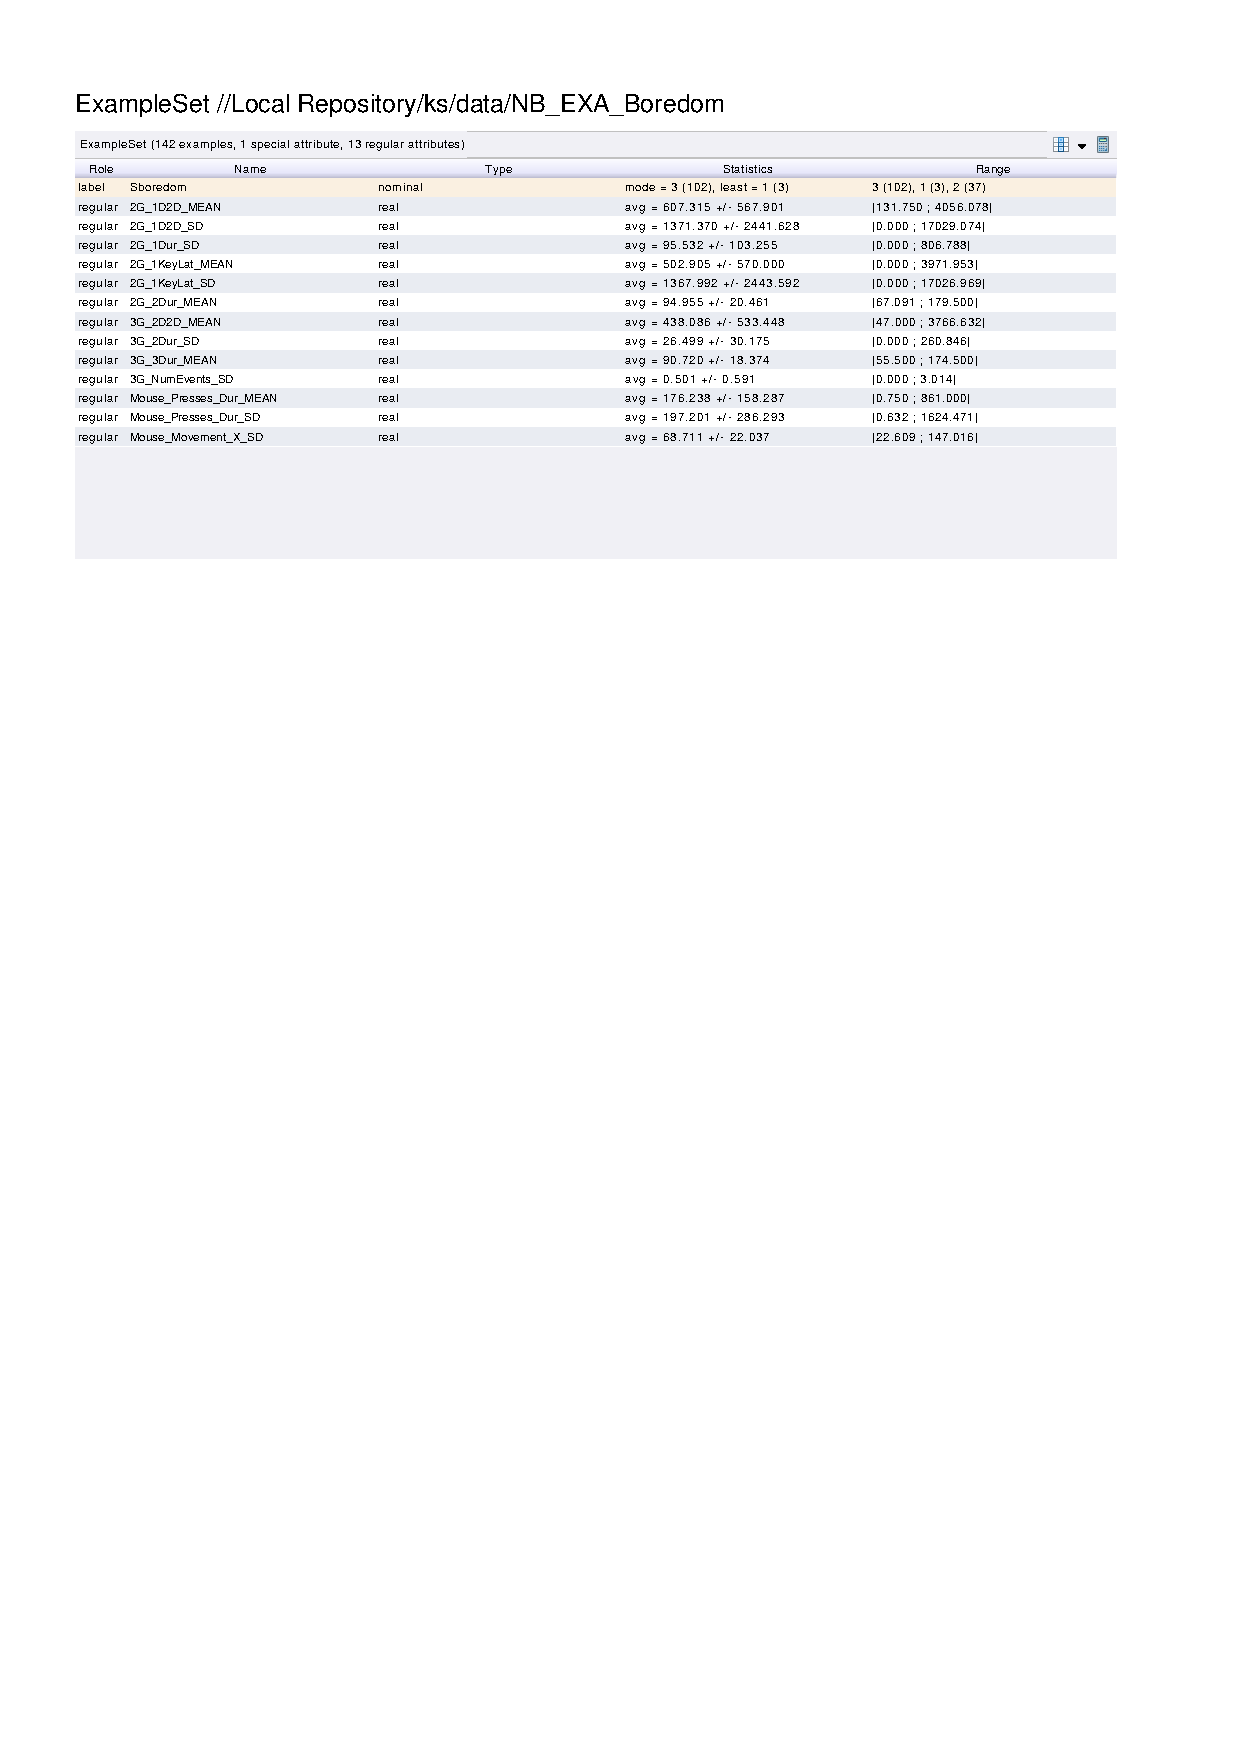
\includegraphics[trim=0 620 0 60,clip,width=16.09cm]{results/NB_EXA_Boredom.pdf}} \caption{
} \label{NB_K_Boredom}
\end{figure}

\begin{figure}[htp]
  \centerline{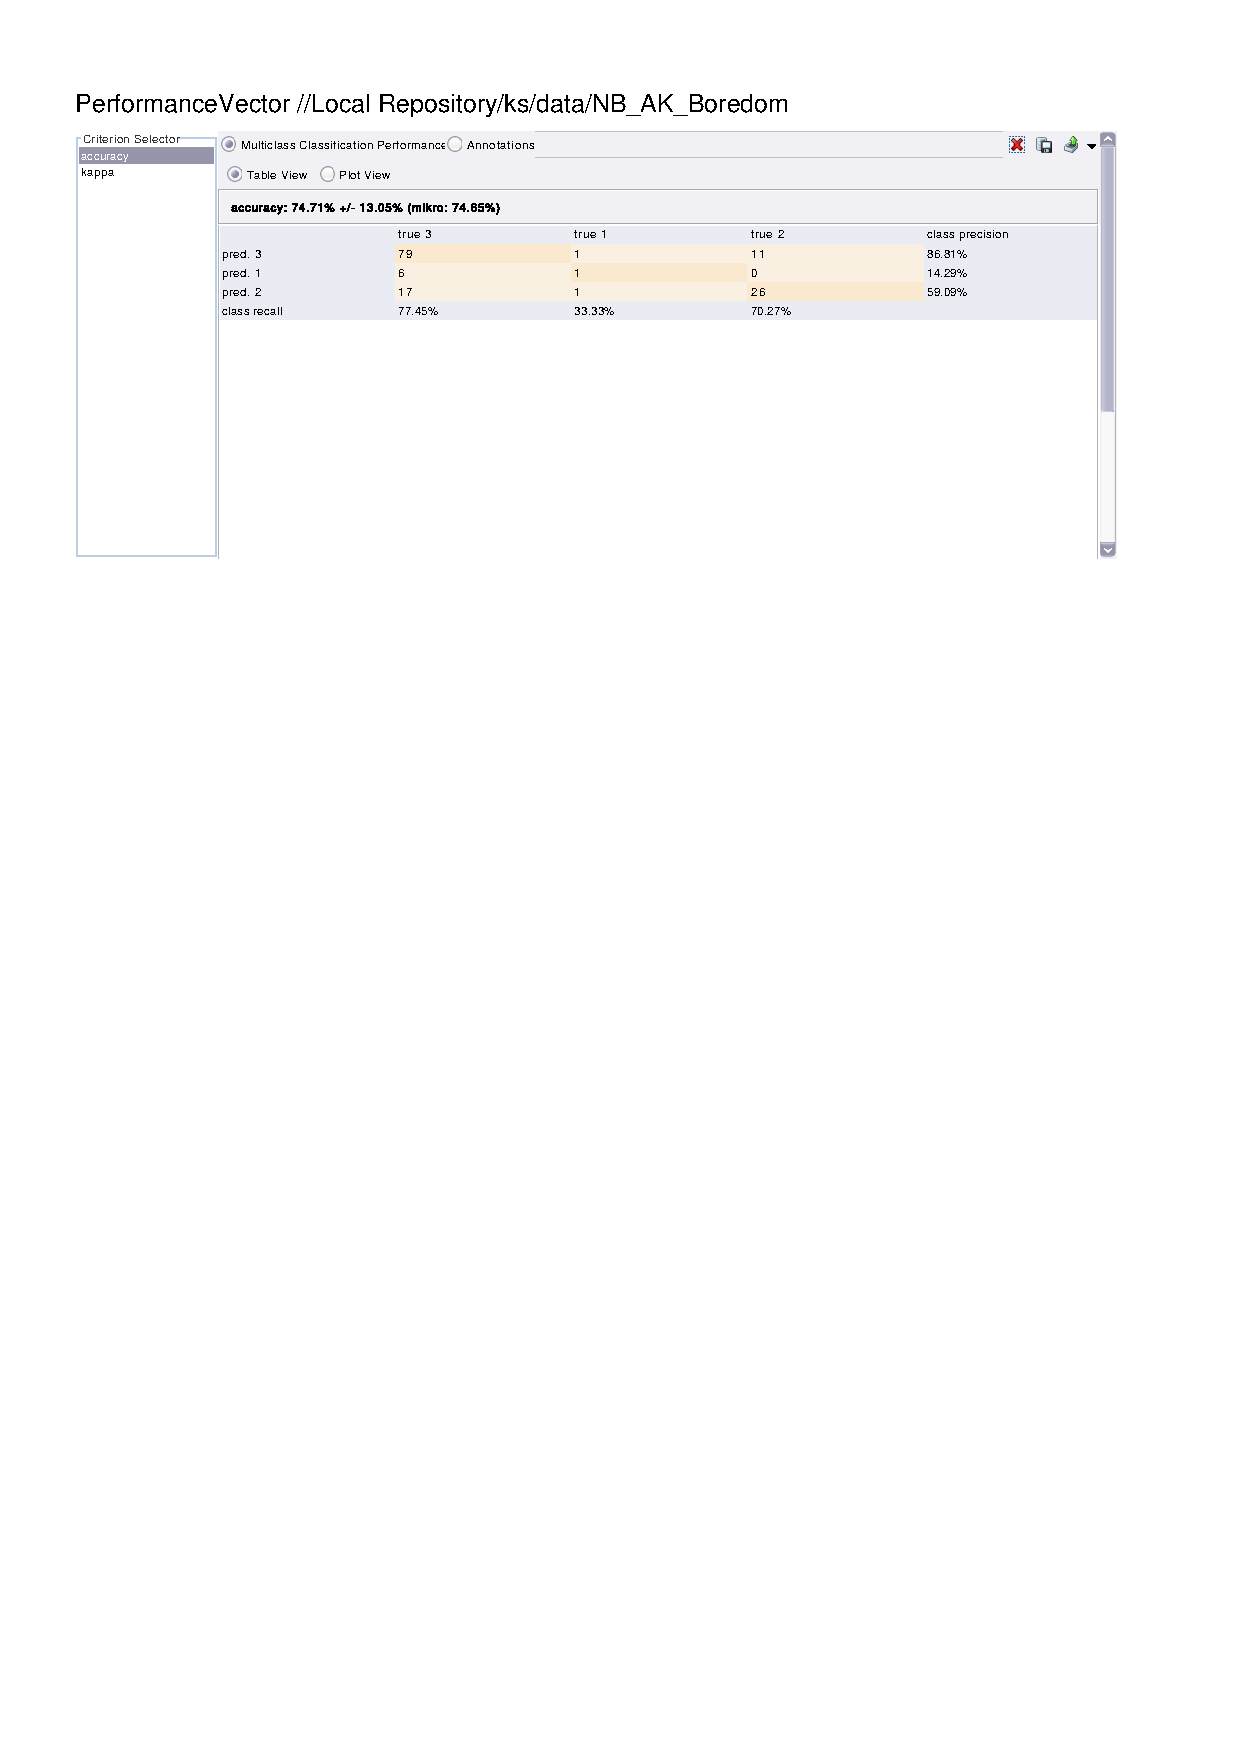
\includegraphics[trim=0 680 0 60,clip,width=16.09cm]{results/NB_A_Boredom.pdf}} \caption{
} \label{NB_K_Boredom}
\end{figure}

\begin{figure}[htp]
  \centerline{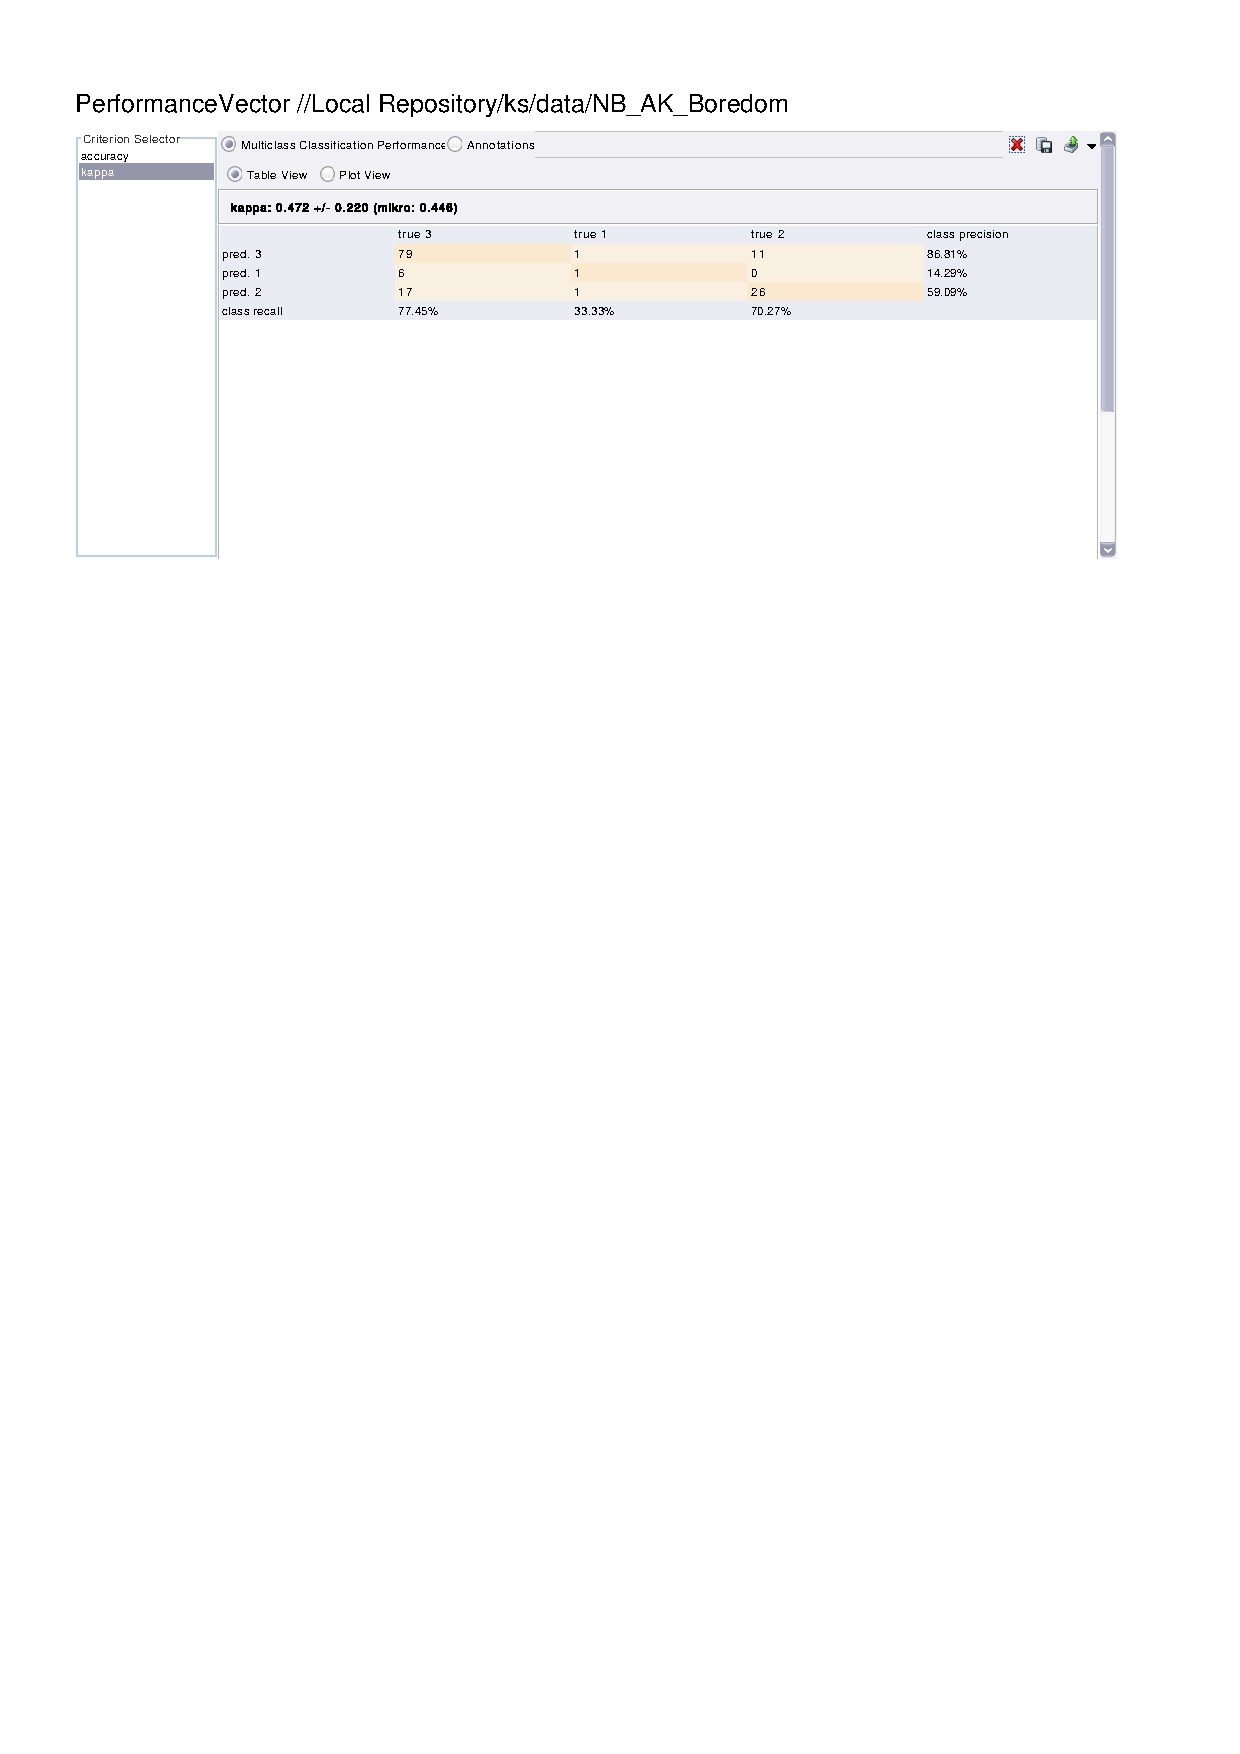
\includegraphics[trim=0 680 0 60,clip,width=16.09cm]{results/NB_K_Boredom.pdf}} \caption{
} \label{NB_K_Boredom}
\end{figure}

\clearpage
\FloatBarrier
% Naive-Bayes Distraction
\subsubsection{Distracción}

\begin{figure}[htp]
  \centerline{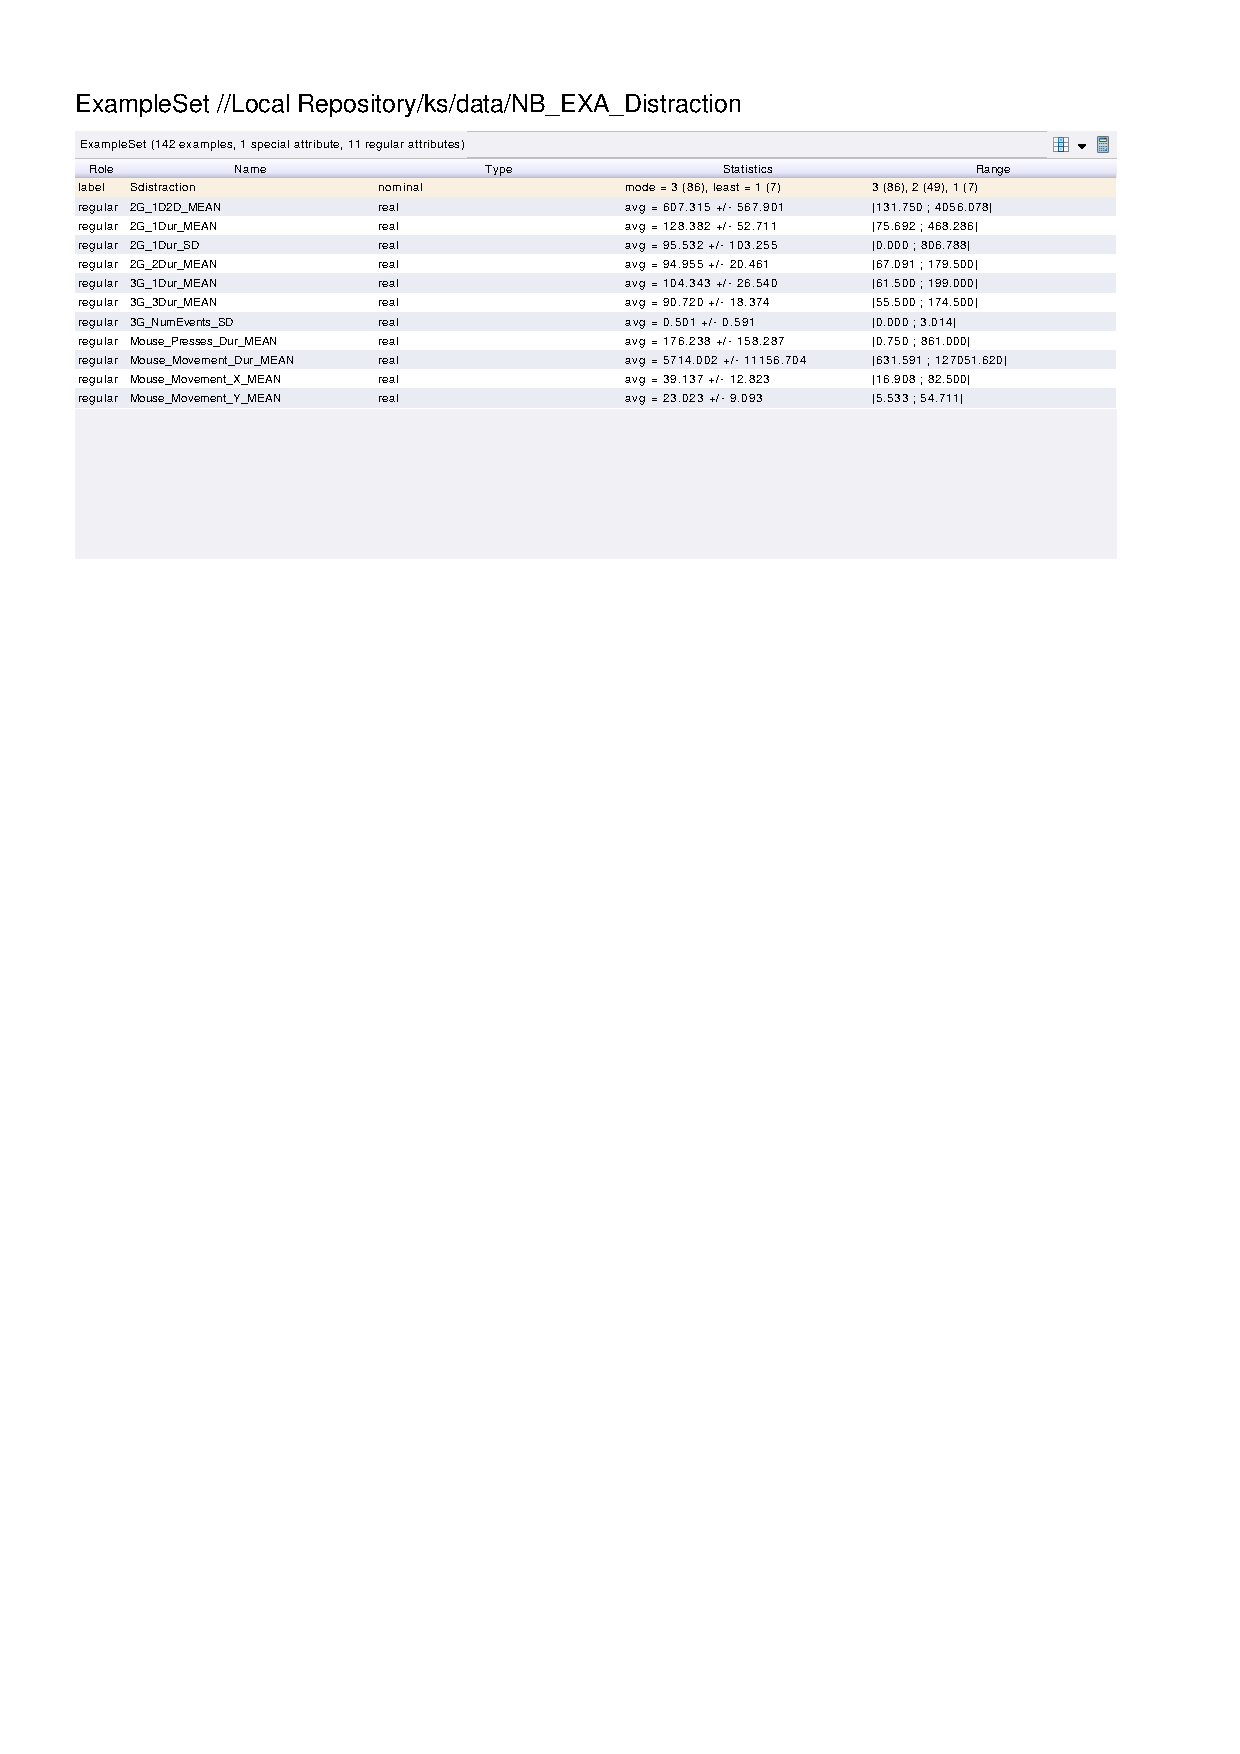
\includegraphics[trim=0 630 0 60,clip,width=16.09cm]{results/NB_EXA_Distraction.pdf}} \caption{
} \label{NB_K_Distraction}
\end{figure}

\begin{figure}[htp]
  \centerline{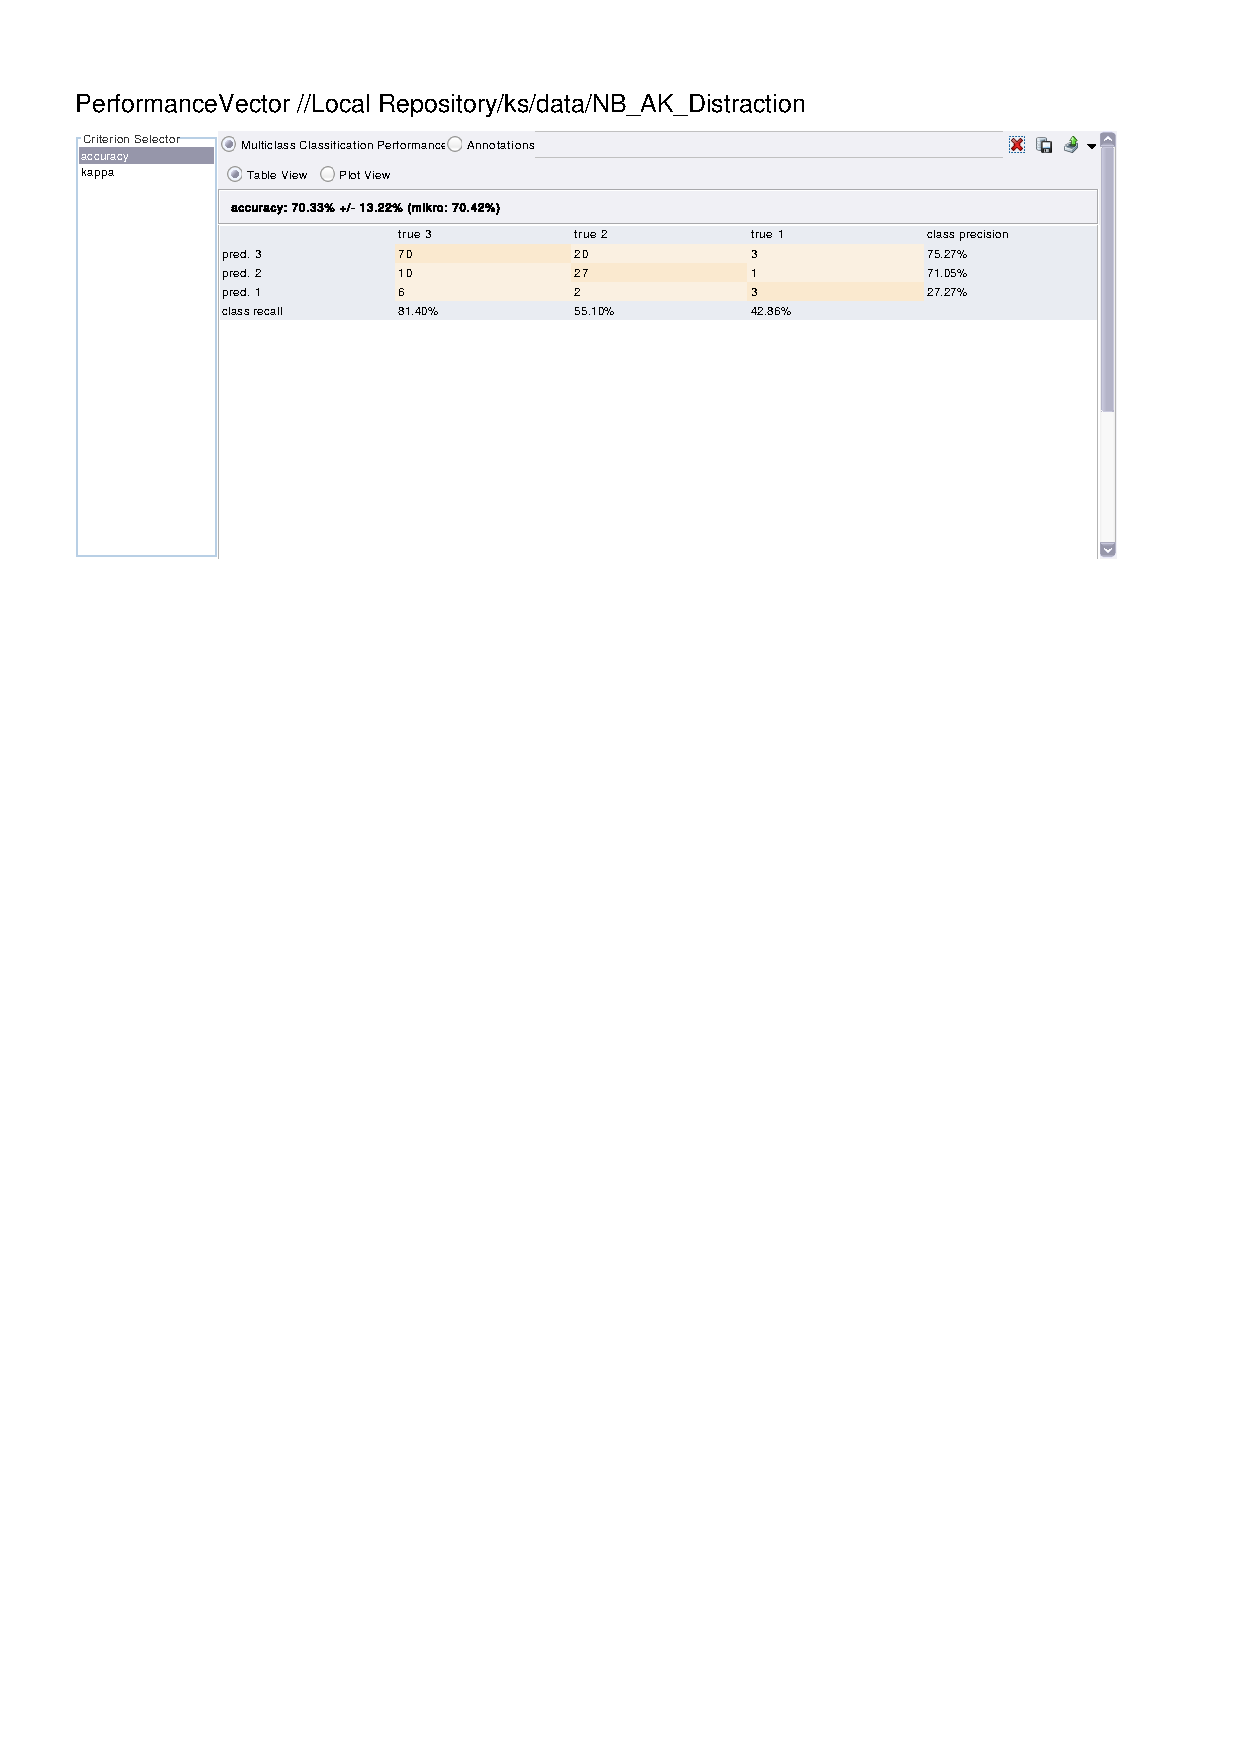
\includegraphics[trim=0 680 0 60,clip,width=16.09cm]{results/NB_A_Distraction.pdf}} \caption{
} \label{NB_K_Distraction}
\end{figure}

\begin{figure}[htp]
  \centerline{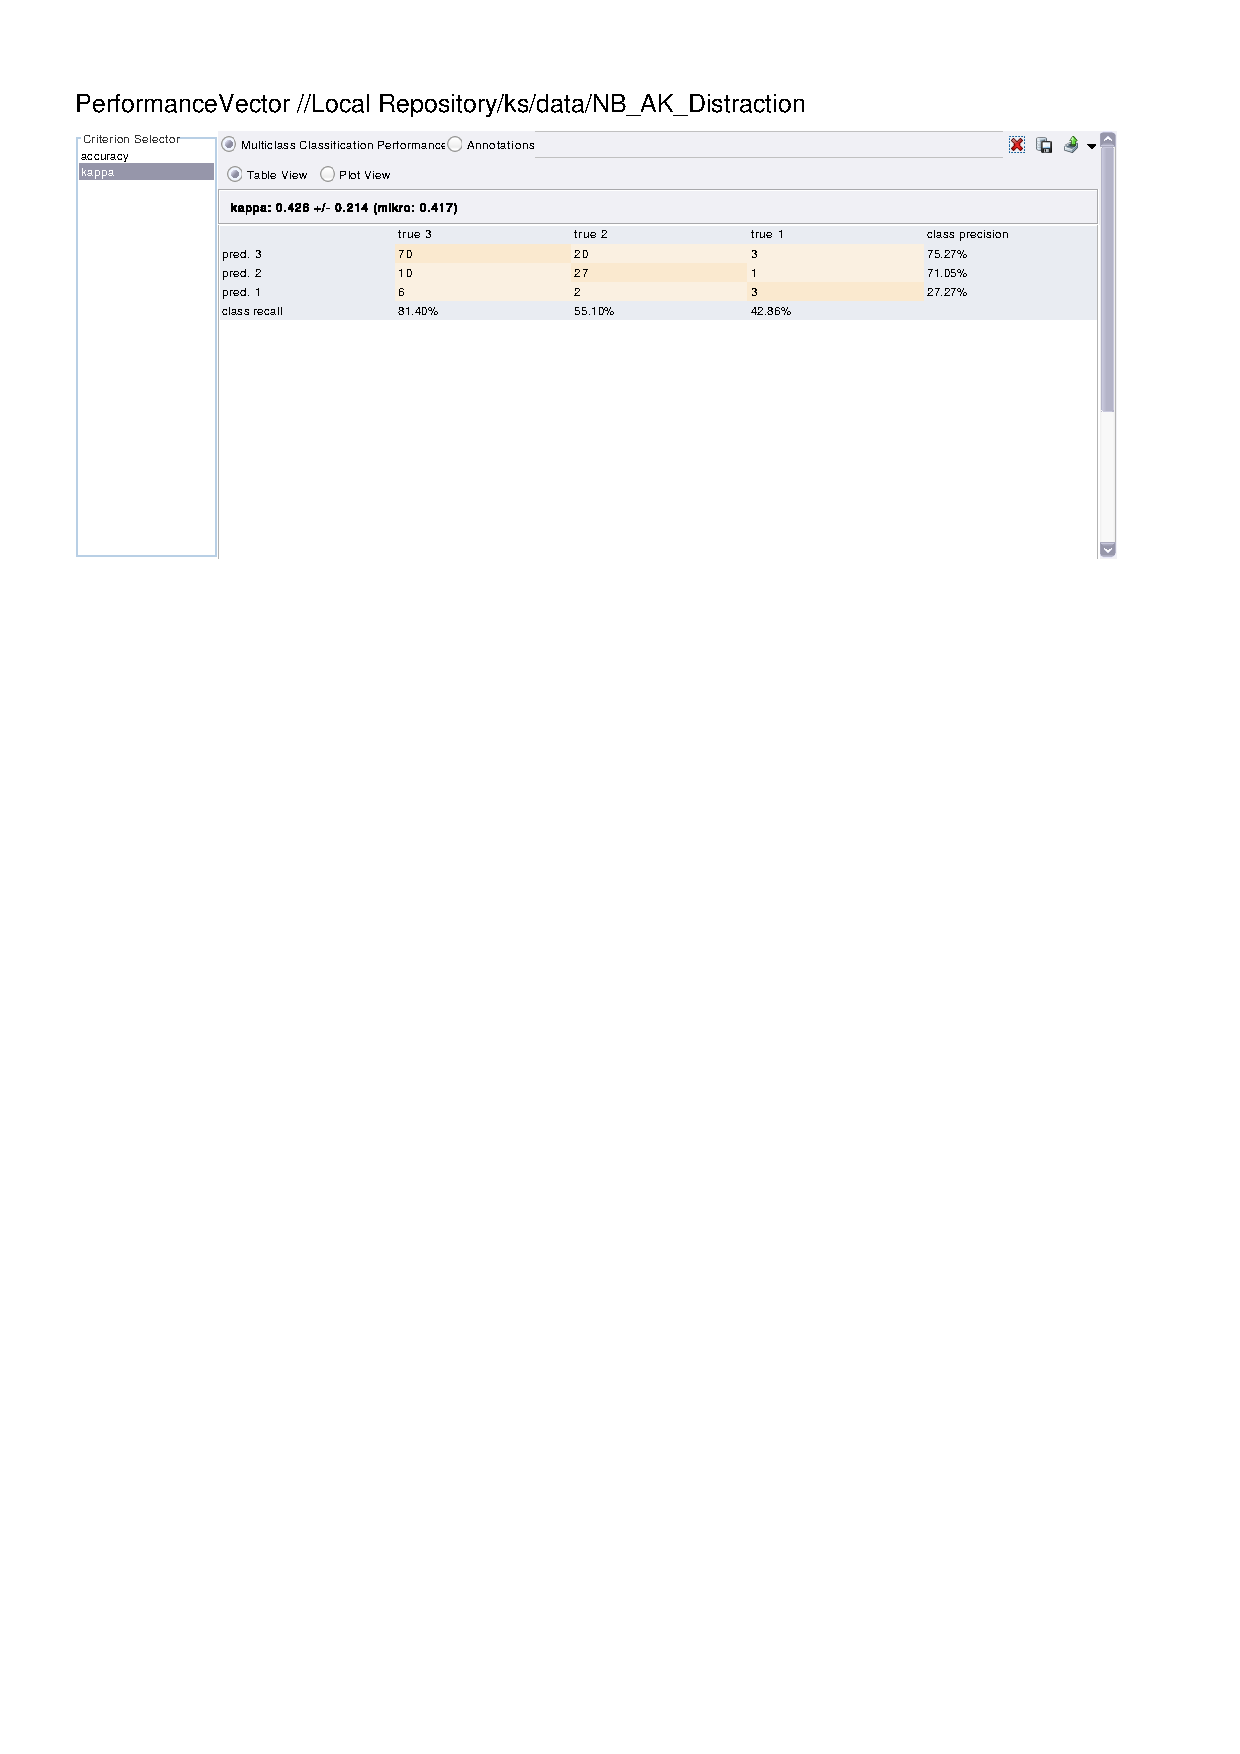
\includegraphics[trim=0 680 0 60,clip,width=16.09cm]{results/NB_K_Distraction.pdf}} \caption{
} \label{NB_K_Distraction}
\end{figure}

\clearpage
\FloatBarrier
% Naive-Bayes Excitement
\subsubsection{Entusiasmo}

\begin{figure}[htp]
  \centerline{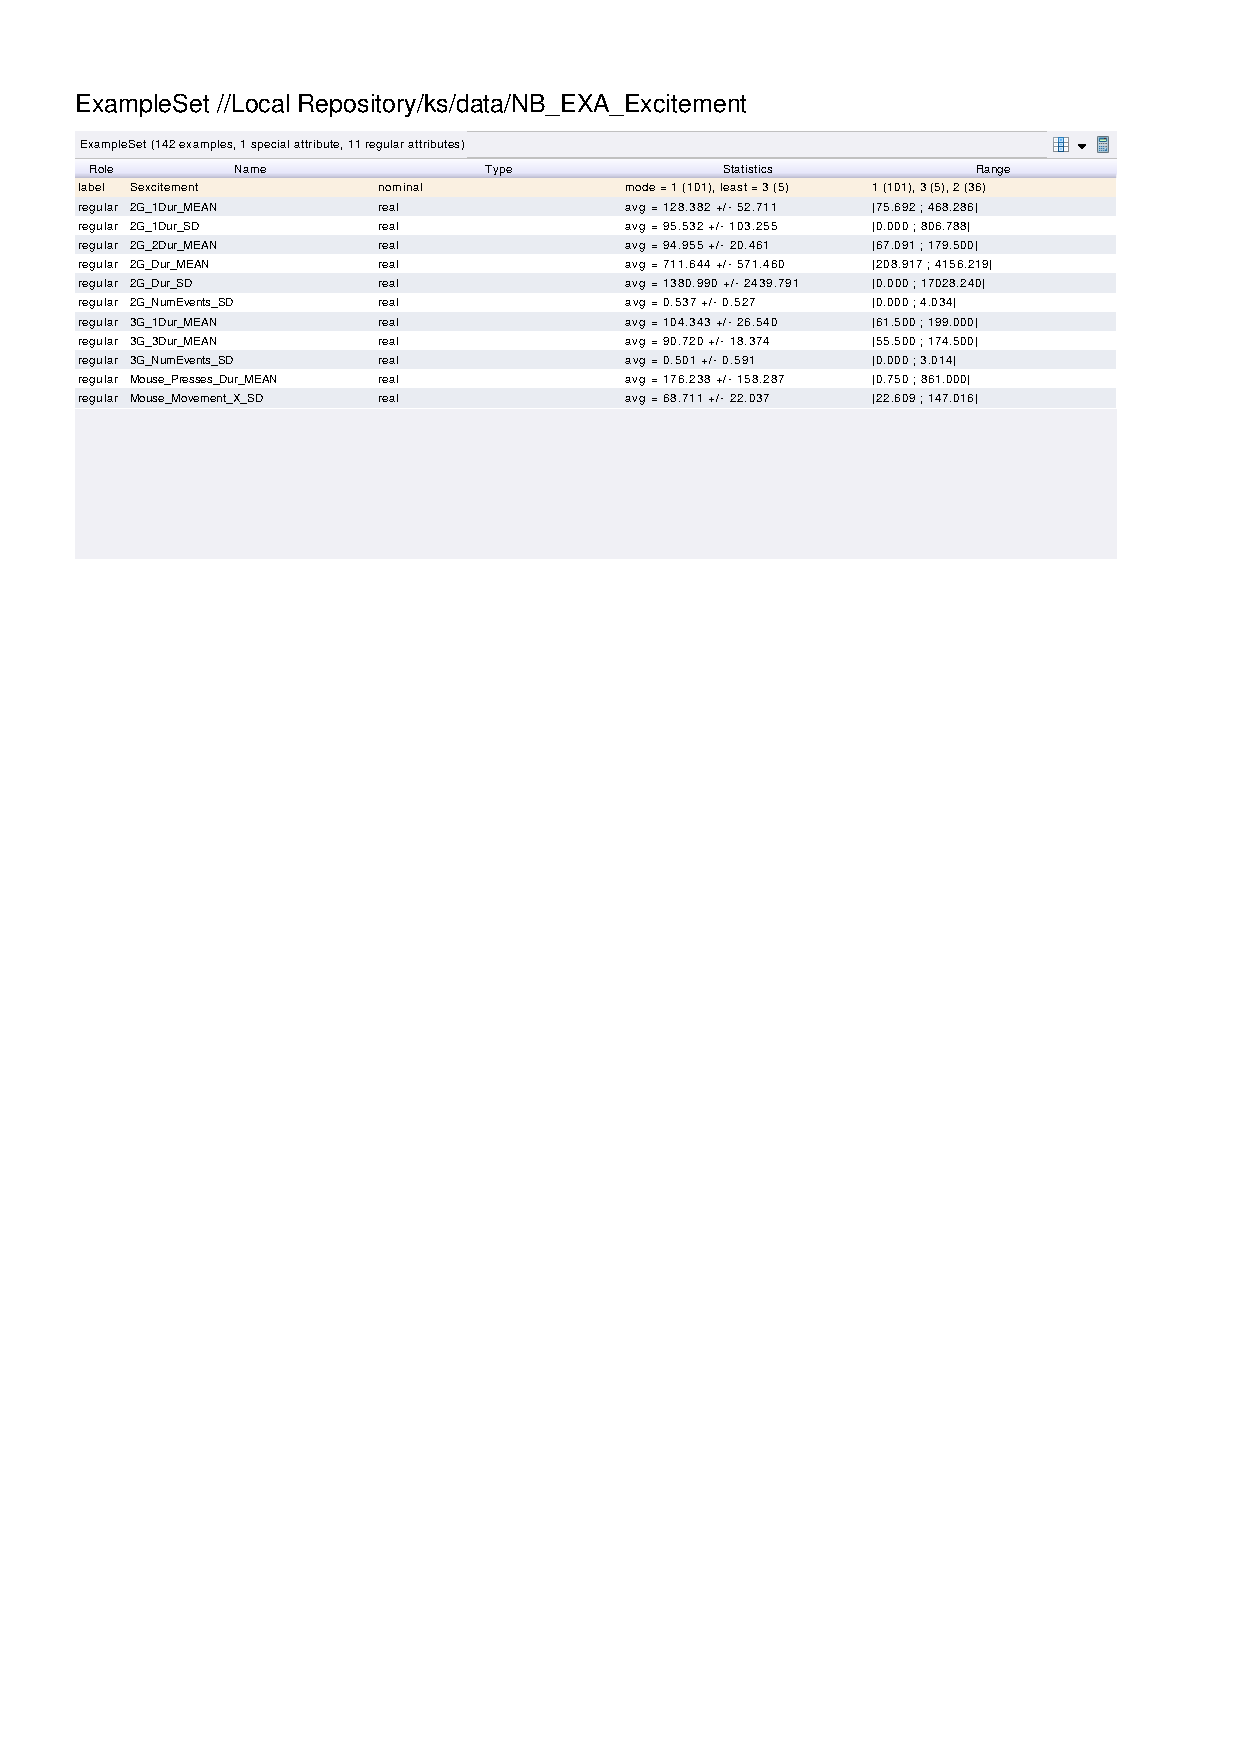
\includegraphics[trim=0 630 0 60,clip,width=16.09cm]{results/NB_EXA_Excitement.pdf}} \caption{
} \label{NB_K_Excitement}
\end{figure}

\begin{figure}[htp]
  \centerline{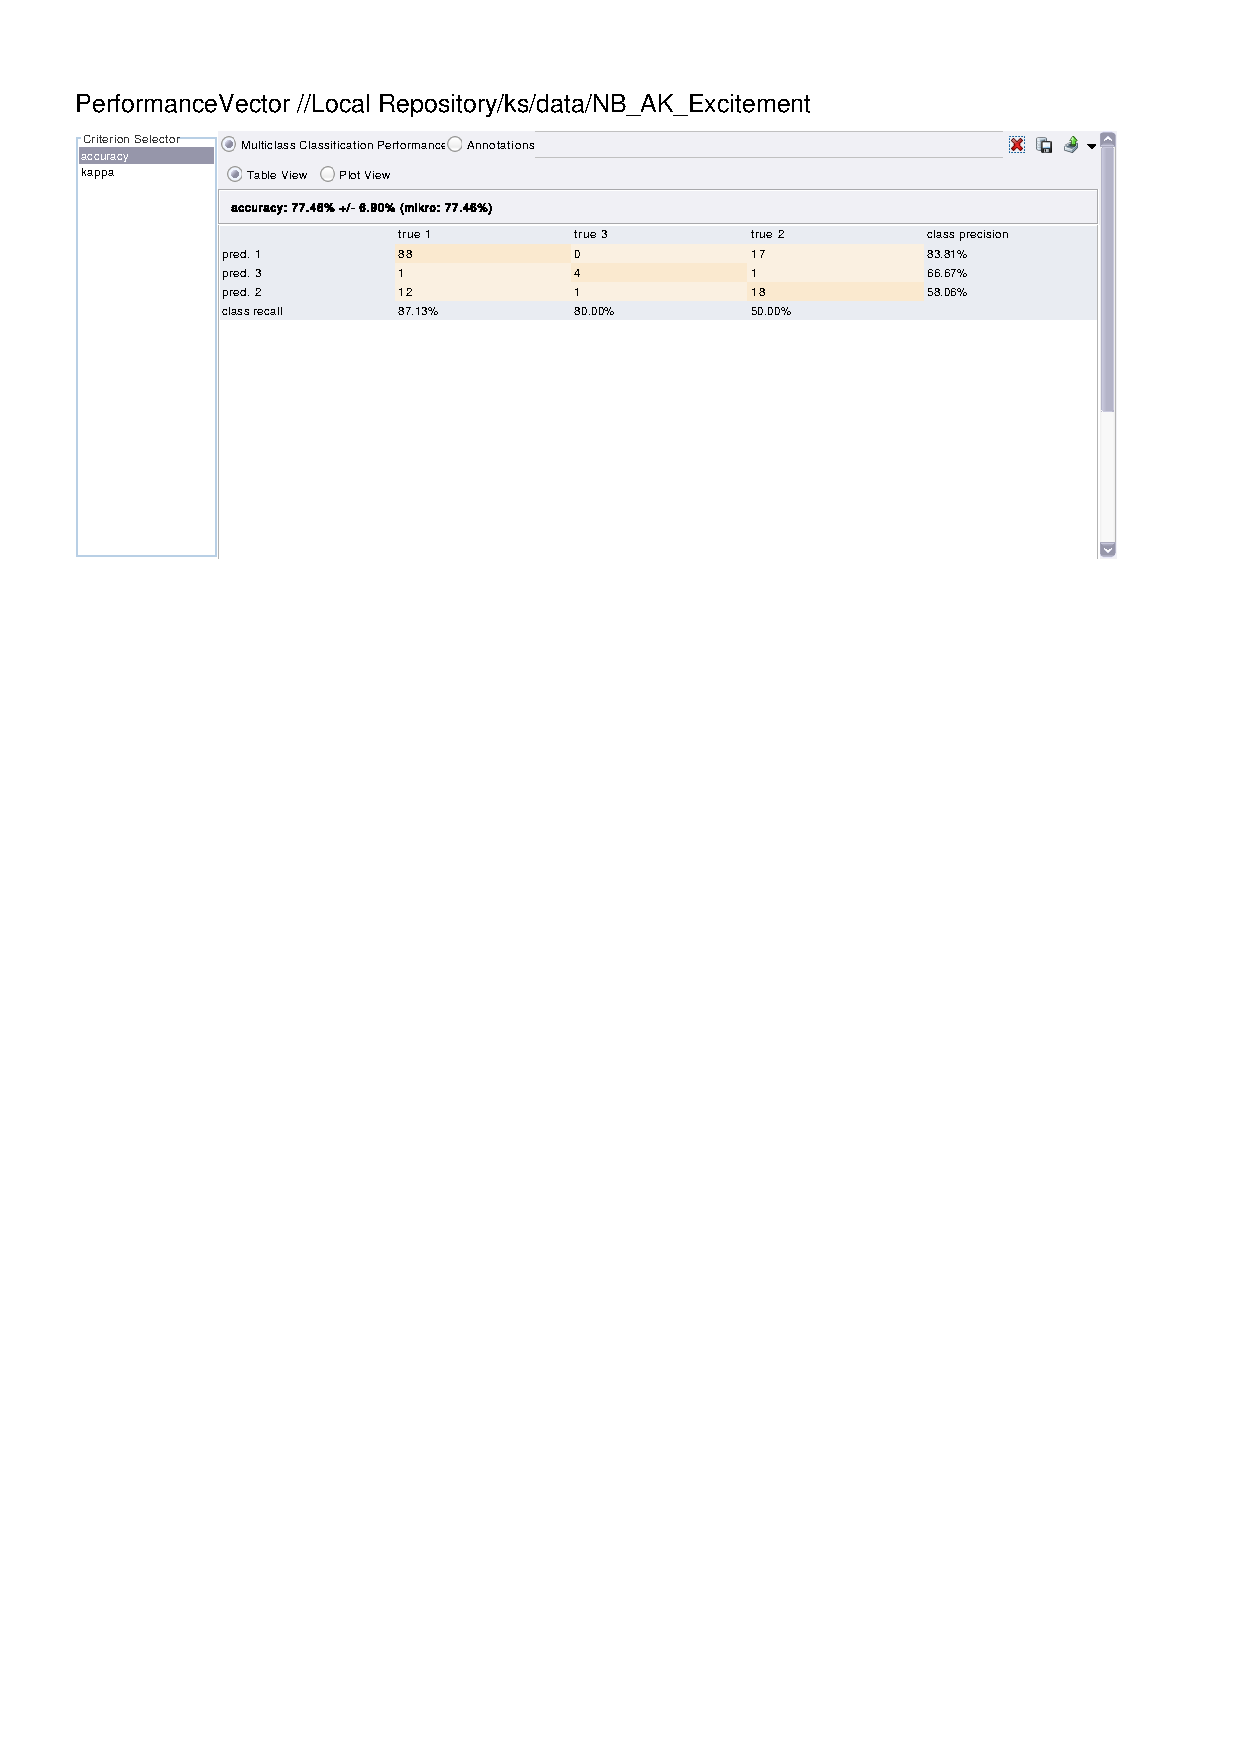
\includegraphics[trim=0 680 0 60,clip,width=16.09cm]{results/NB_A_Excitement.pdf}} \caption{
} \label{NB_K_Excitement}
\end{figure}

\begin{figure}[htp]
  \centerline{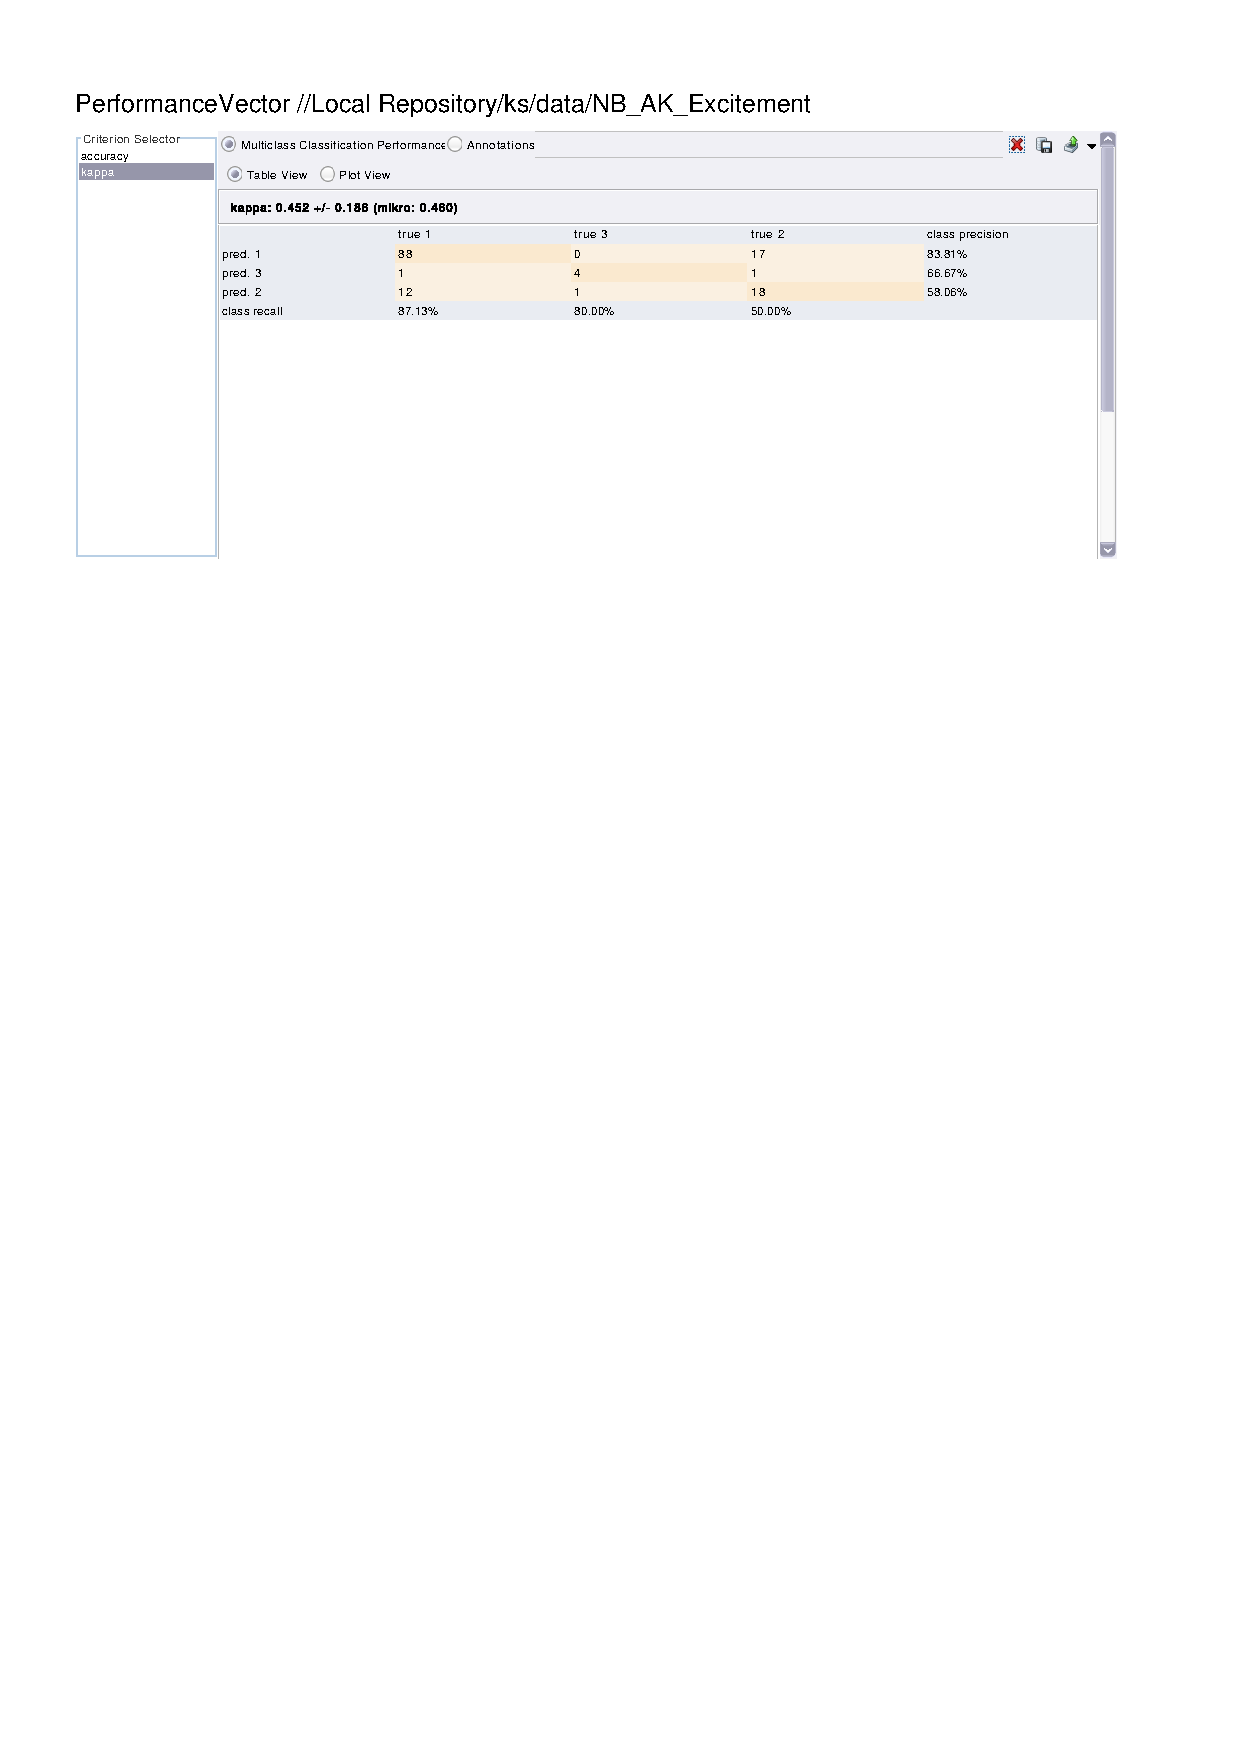
\includegraphics[trim=0 680 0 60,clip,width=16.09cm]{results/NB_K_Excitement.pdf}} \caption{
} \label{NB_K_Excitement}
\end{figure}

\clearpage
\FloatBarrier
% Naive-Bayes Focus
\subsubsection{Concentración}

\begin{figure}[htp]
  \centerline{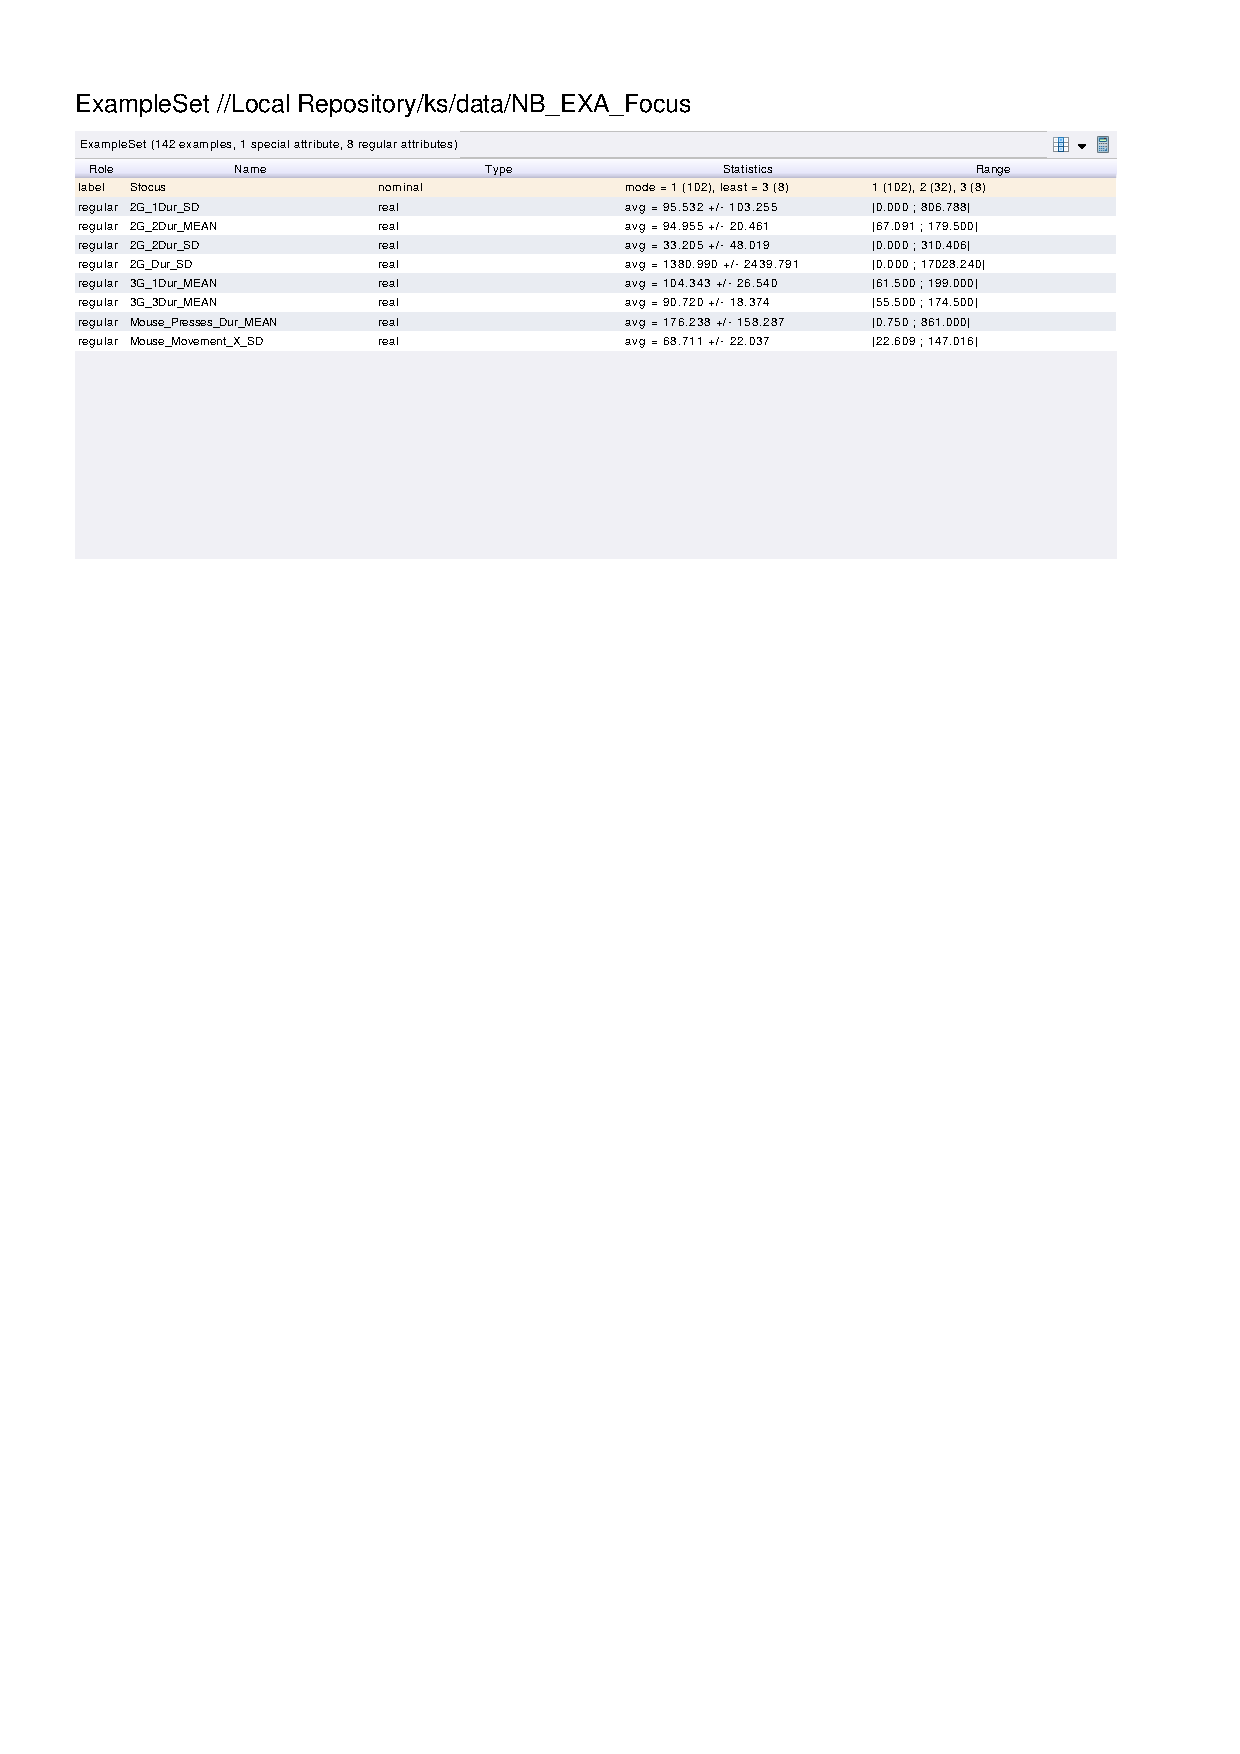
\includegraphics[trim=0 650 0 60,clip,width=16.09cm]{results/NB_EXA_Focus.pdf}} \caption{
} \label{NB_K_Focus}
\end{figure}

\begin{figure}[htp]
  \centerline{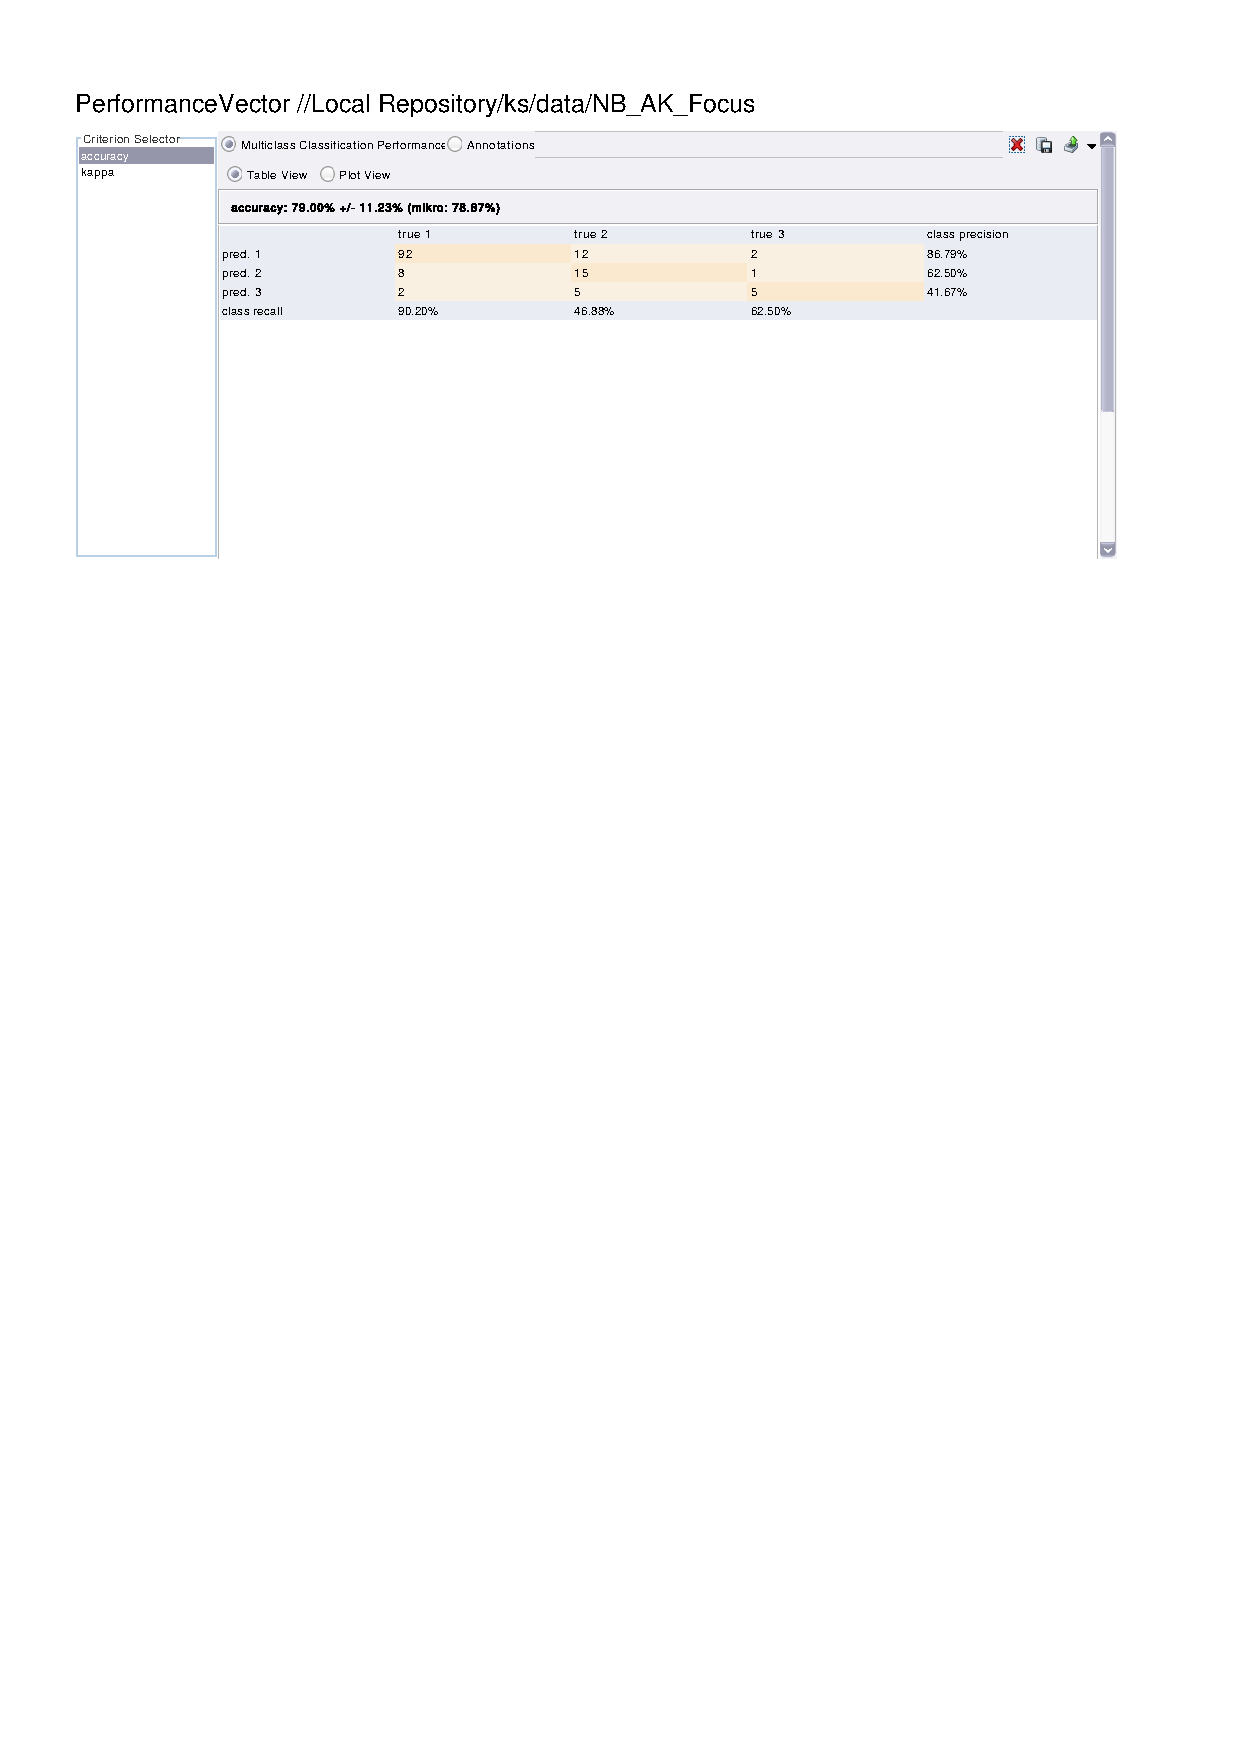
\includegraphics[trim=0 680 0 60,clip,width=16.09cm]{results/NB_A_Focus.pdf}} \caption{
} \label{NB_K_Focus}
\end{figure}

\begin{figure}[htp]
  \centerline{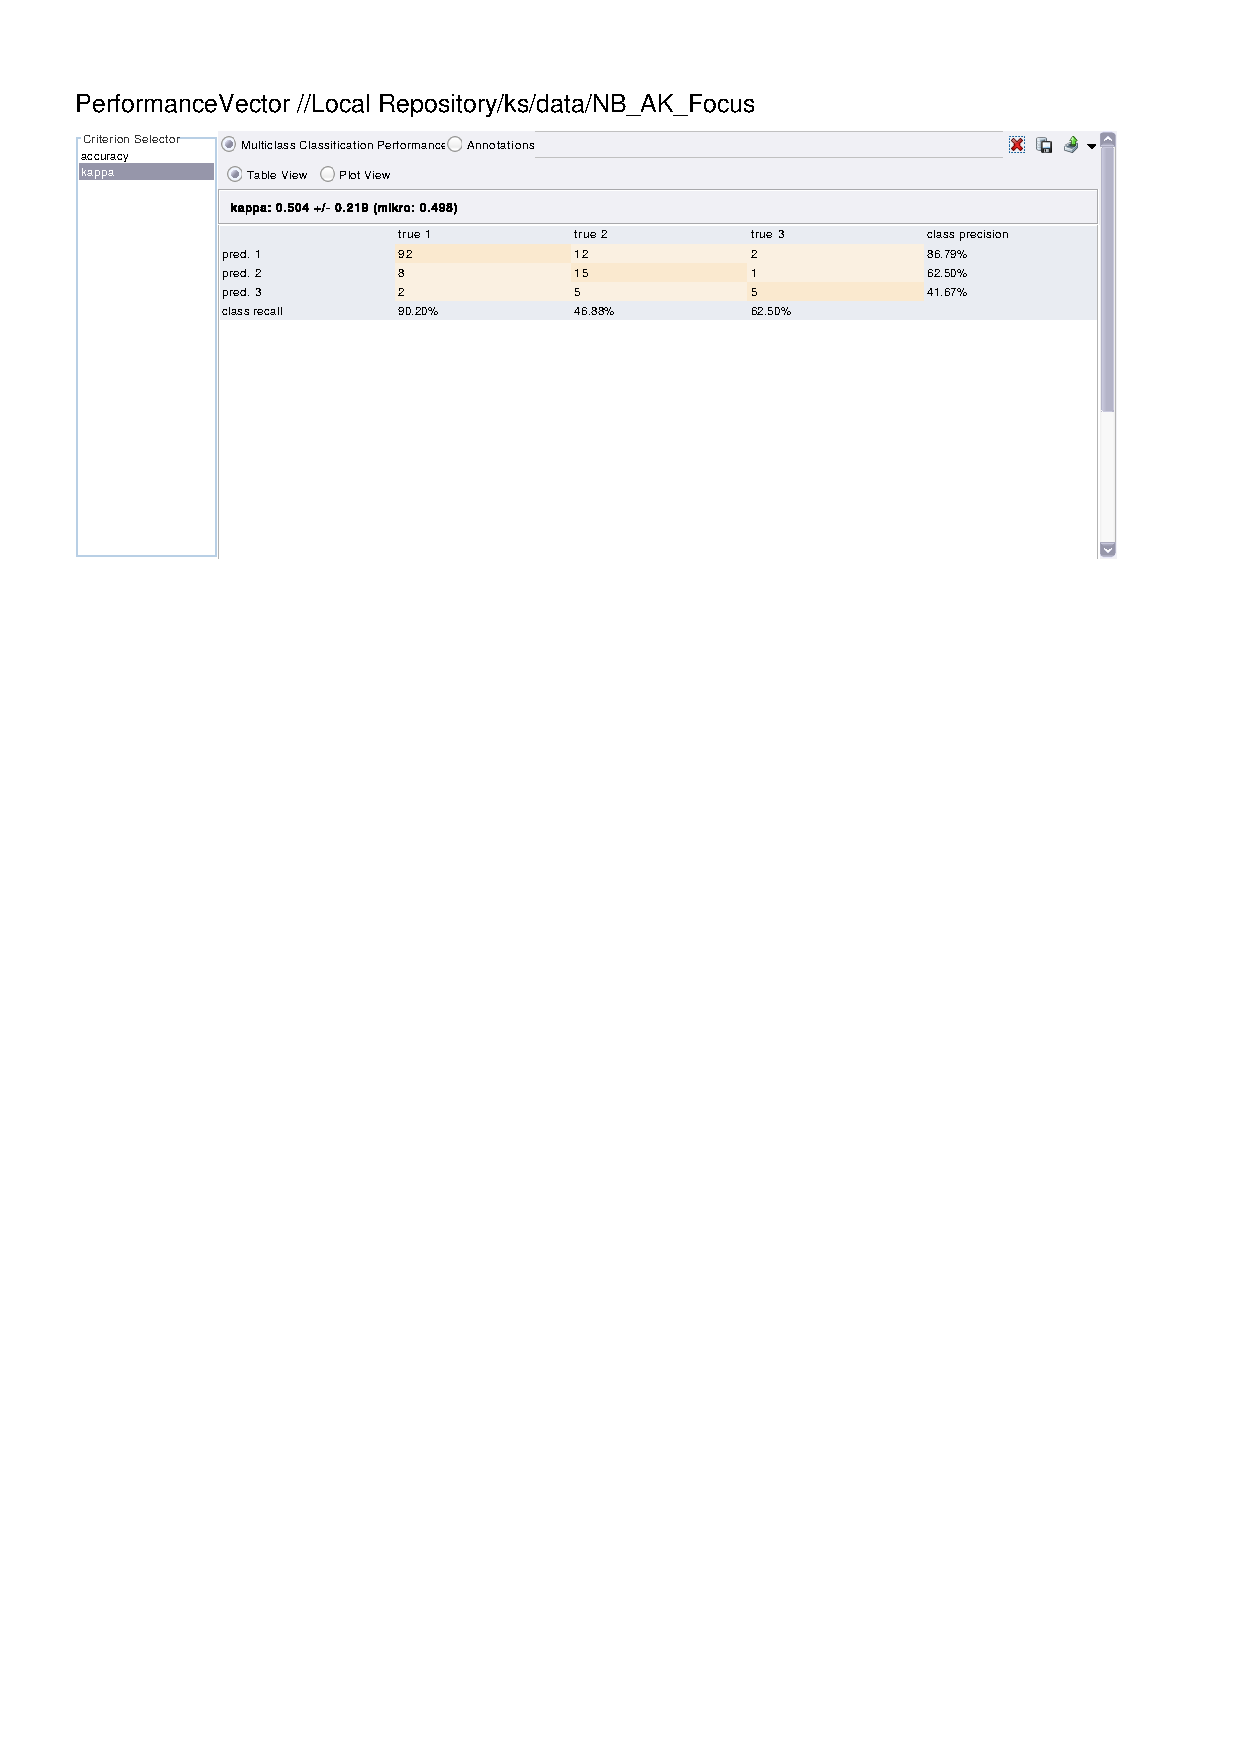
\includegraphics[trim=0 680 0 60,clip,width=16.09cm]{results/NB_K_Focus.pdf}} \caption{
} \label{NB_K_Focus}
\end{figure}

\clearpage
\FloatBarrier
% Naive-Bayes Frustration
\subsubsection{Frustración}

\begin{figure}[htp]
  \centerline{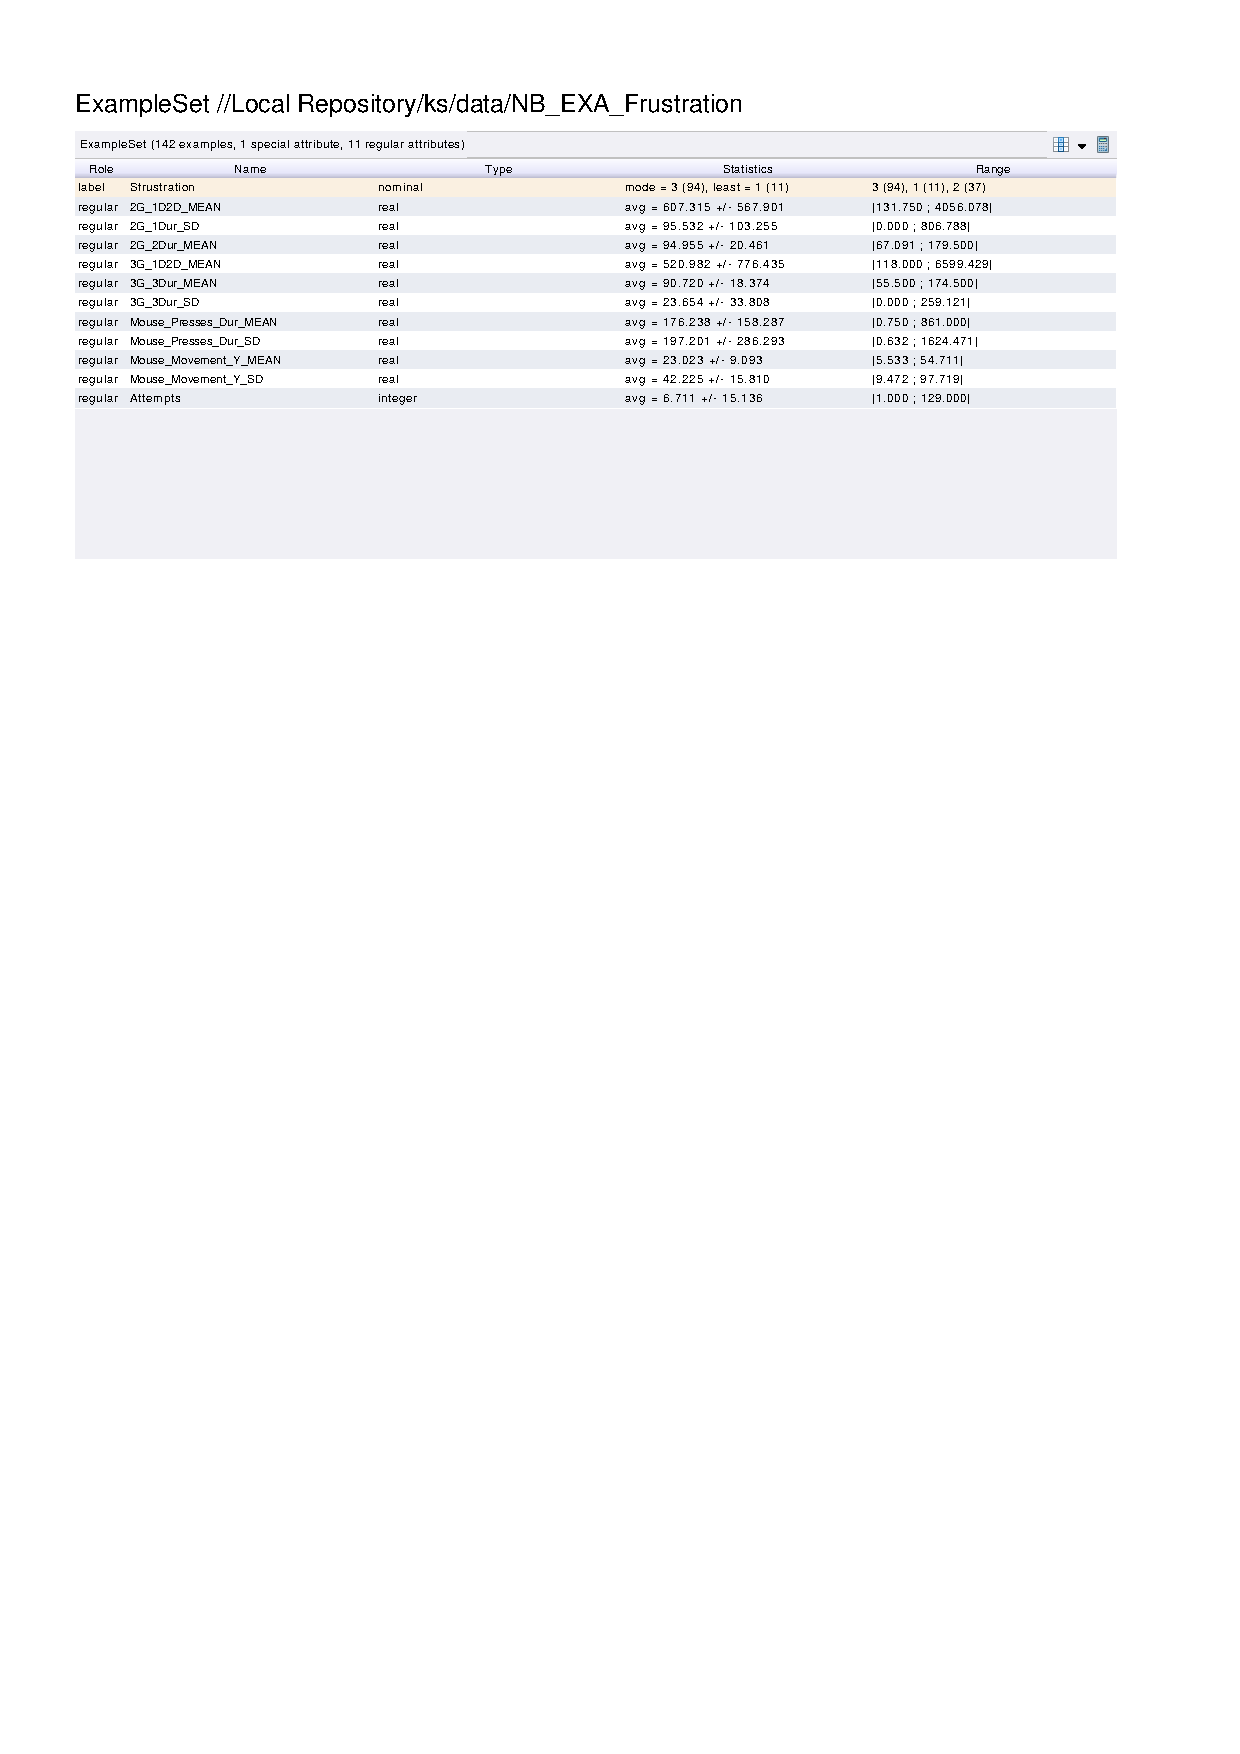
\includegraphics[trim=0 640 0 60,clip,width=16.09cm]{results/NB_EXA_Frustration.pdf}} \caption{
} \label{NB_K_Frustration}
\end{figure}

\begin{figure}[htp]
  \centerline{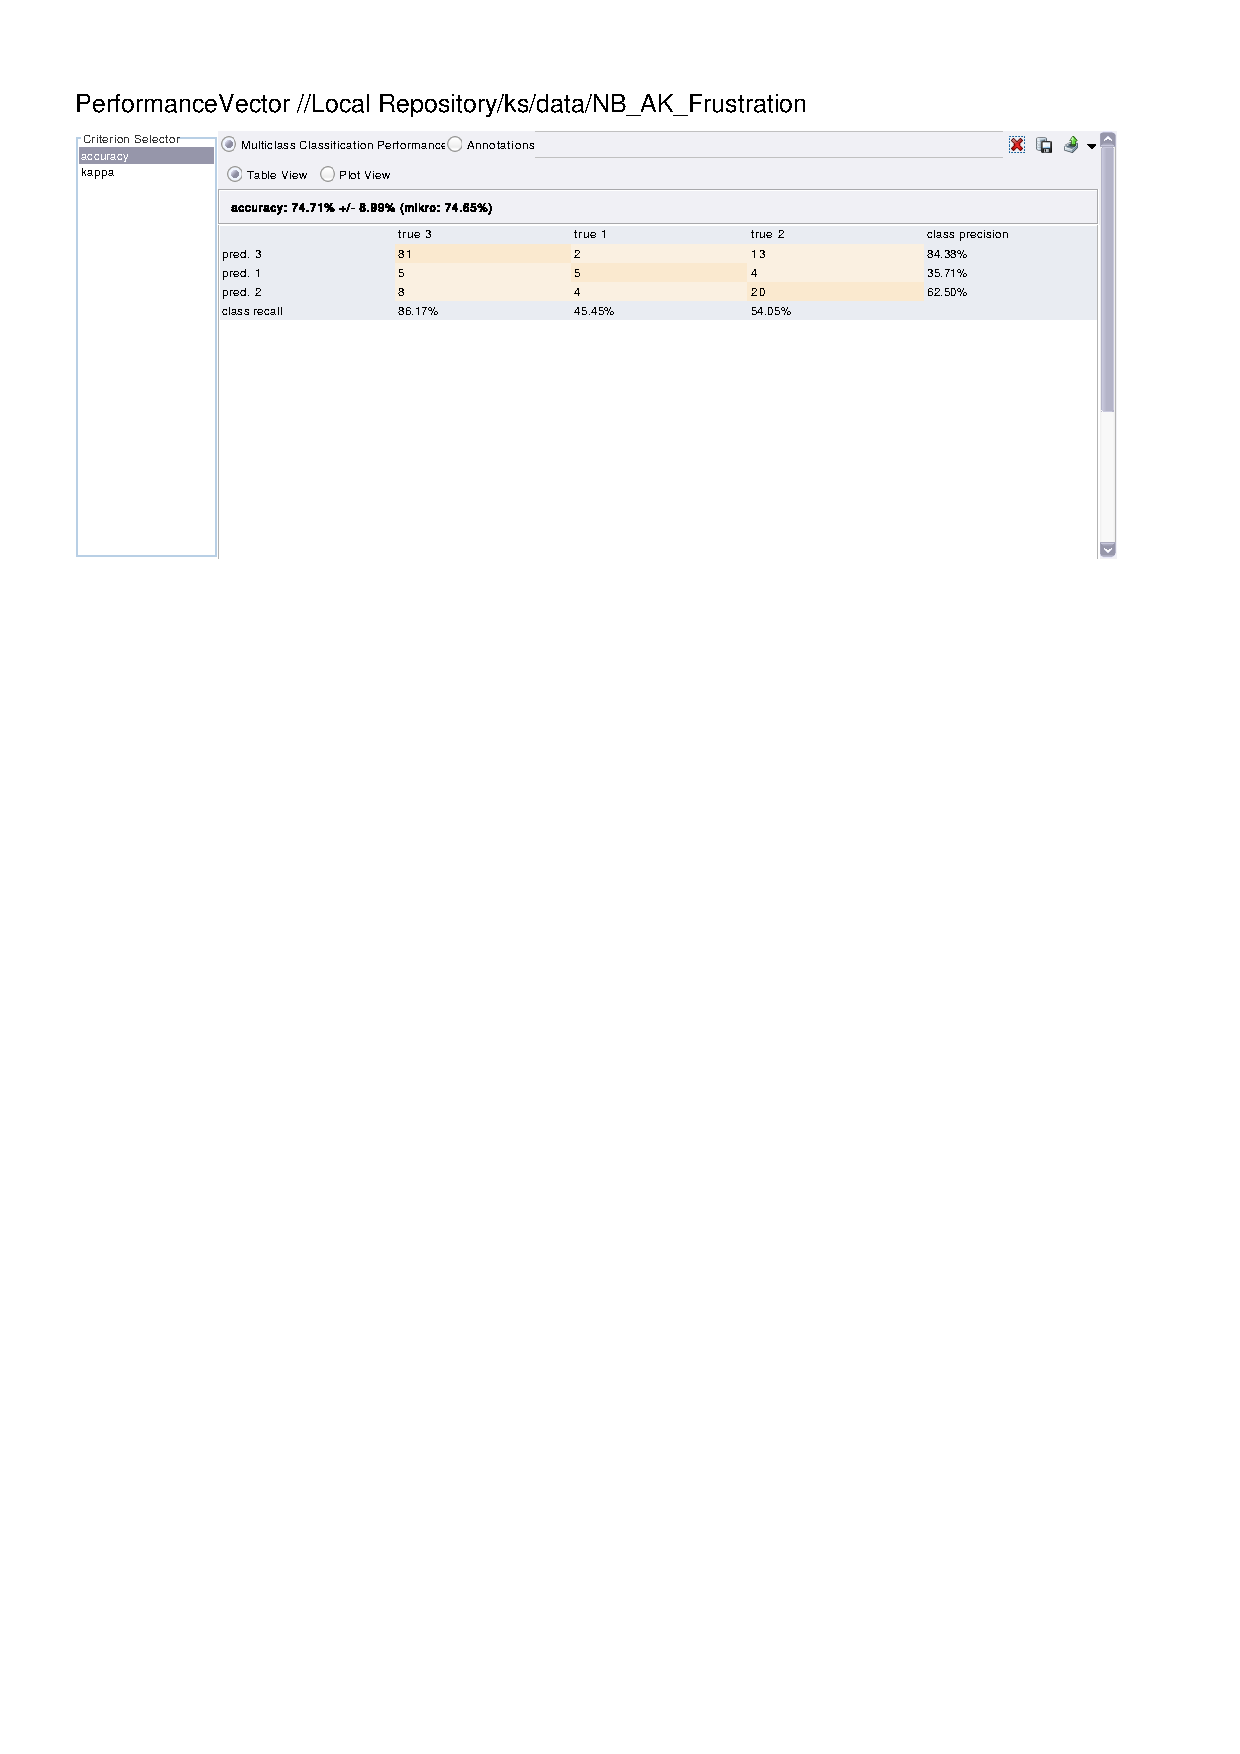
\includegraphics[trim=0 680 0 60,clip,width=16.09cm]{results/NB_A_Frustration.pdf}} \caption{
} \label{NB_K_Frustration}
\end{figure}

\begin{figure}[htp]
  \centerline{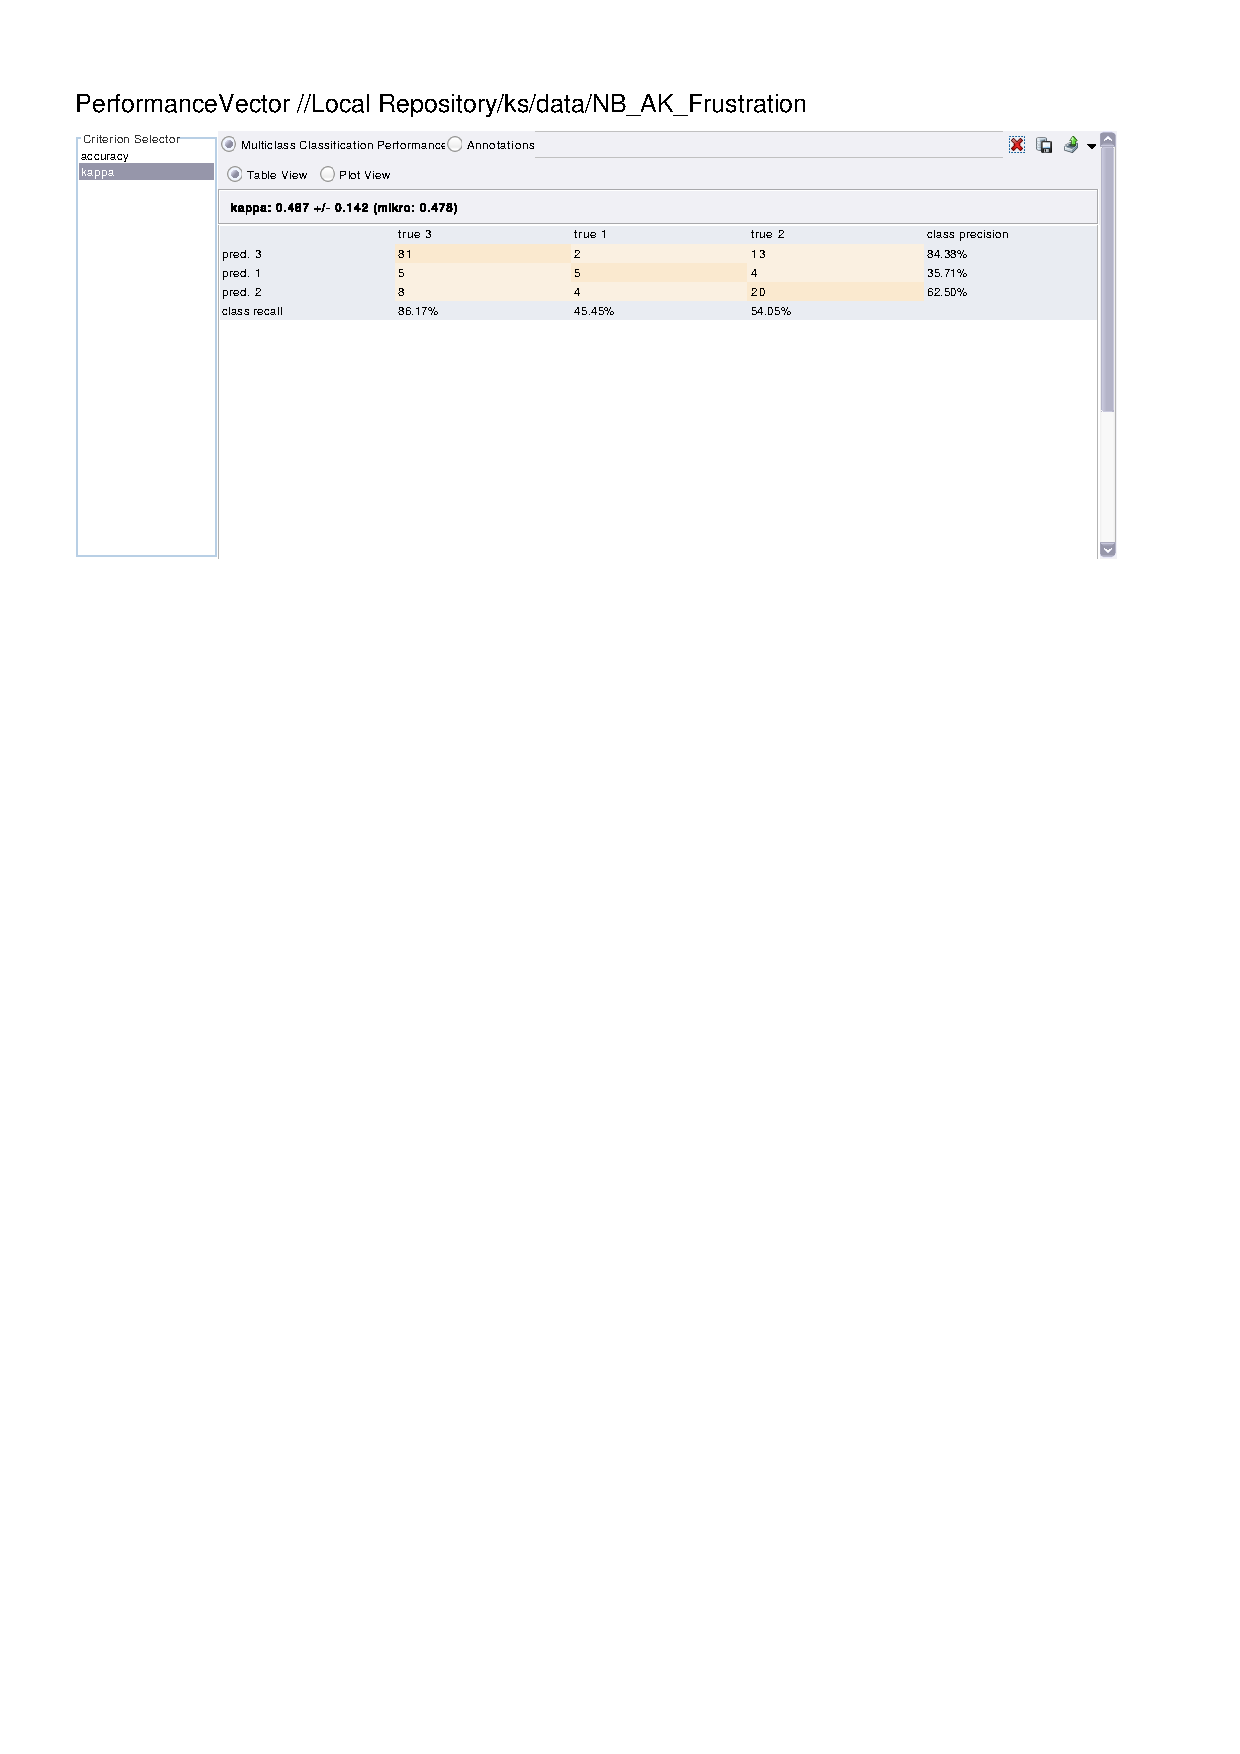
\includegraphics[trim=0 680 0 60,clip,width=16.09cm]{results/NB_K_Frustration.pdf}} \caption{
} \label{NB_K_Frustration}
\end{figure}

\clearpage
\FloatBarrier
% Naive-Bayes Relaxation
\subsubsection{Relajamiento}

\begin{figure}[htp]
  \centerline{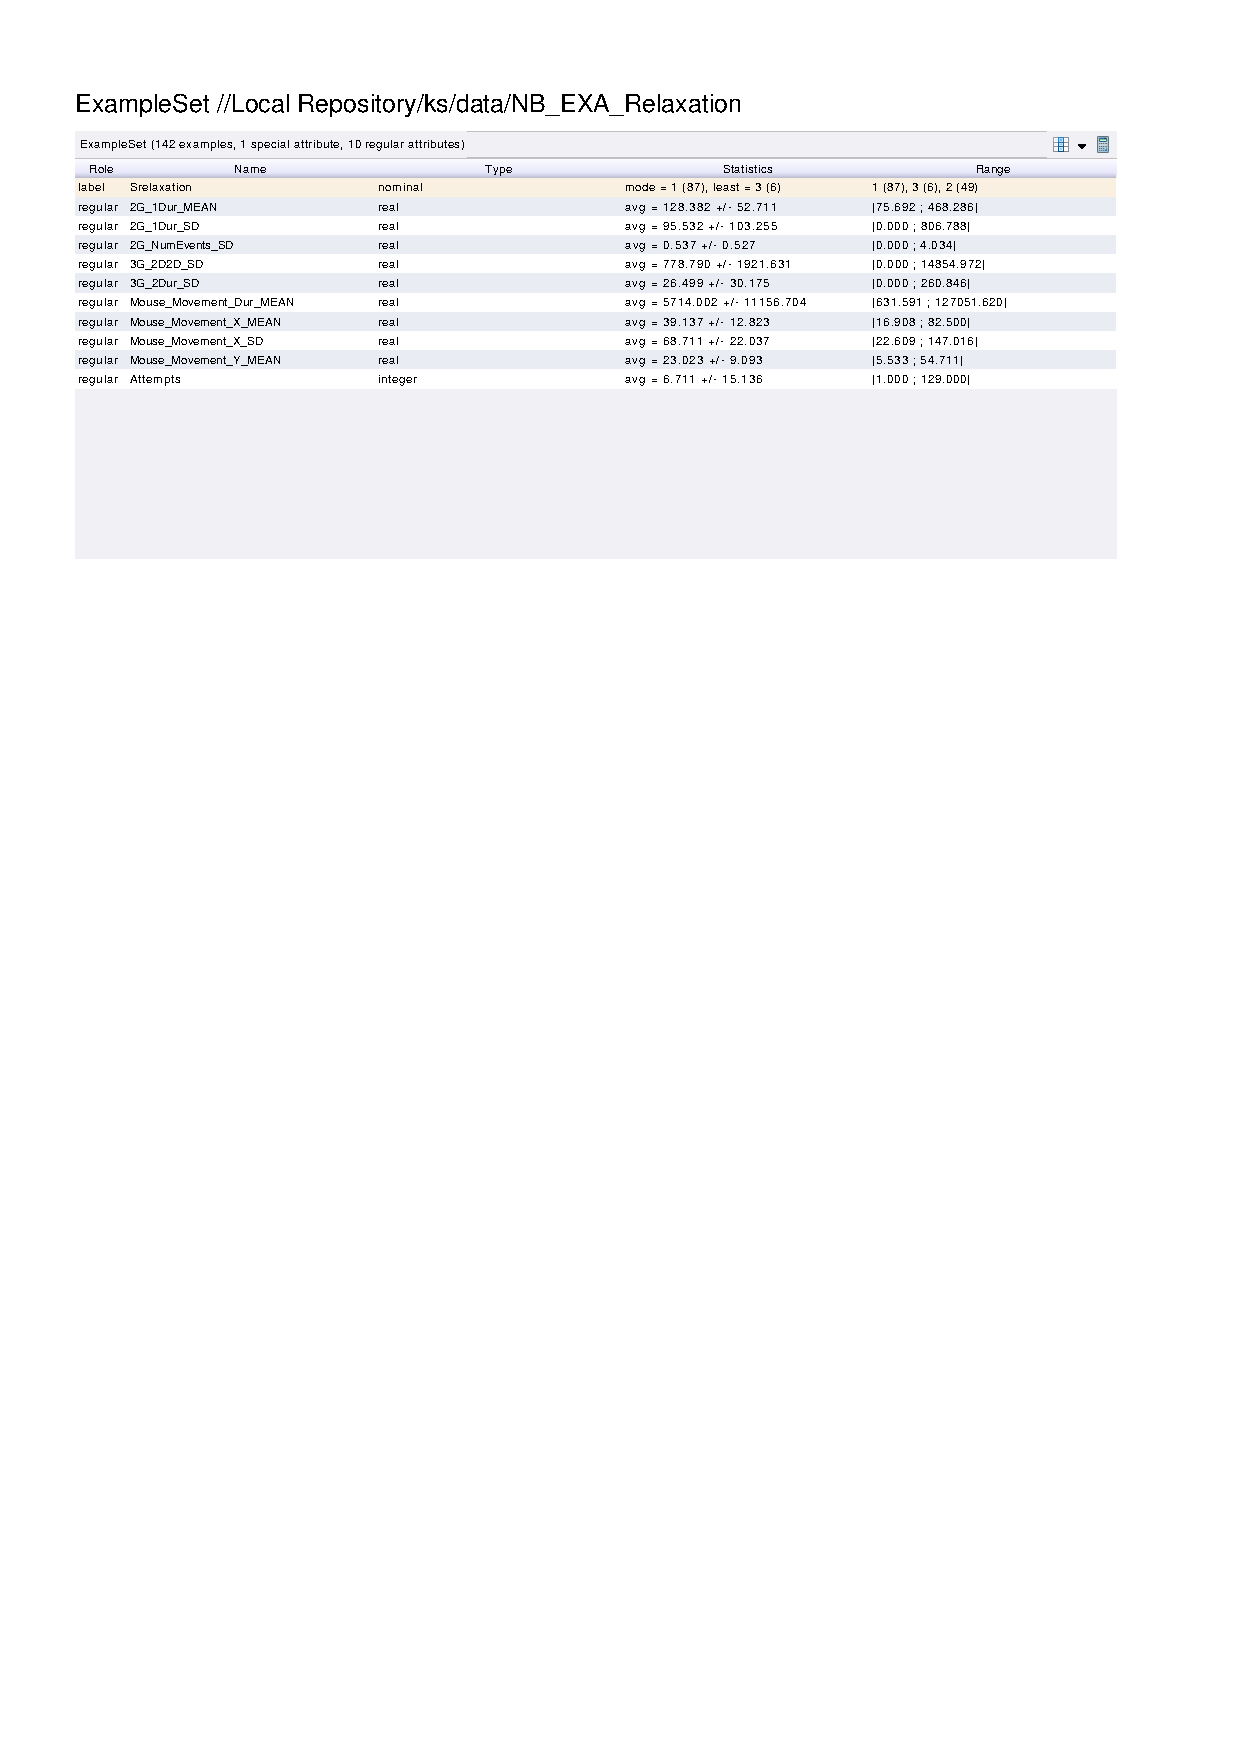
\includegraphics[trim=0 640 0 60,clip,width=16.09cm]{results/NB_EXA_Relaxation.pdf}} \caption{
} \label{NB_K_Relaxation}
\end{figure}

\begin{figure}[htp]
  \centerline{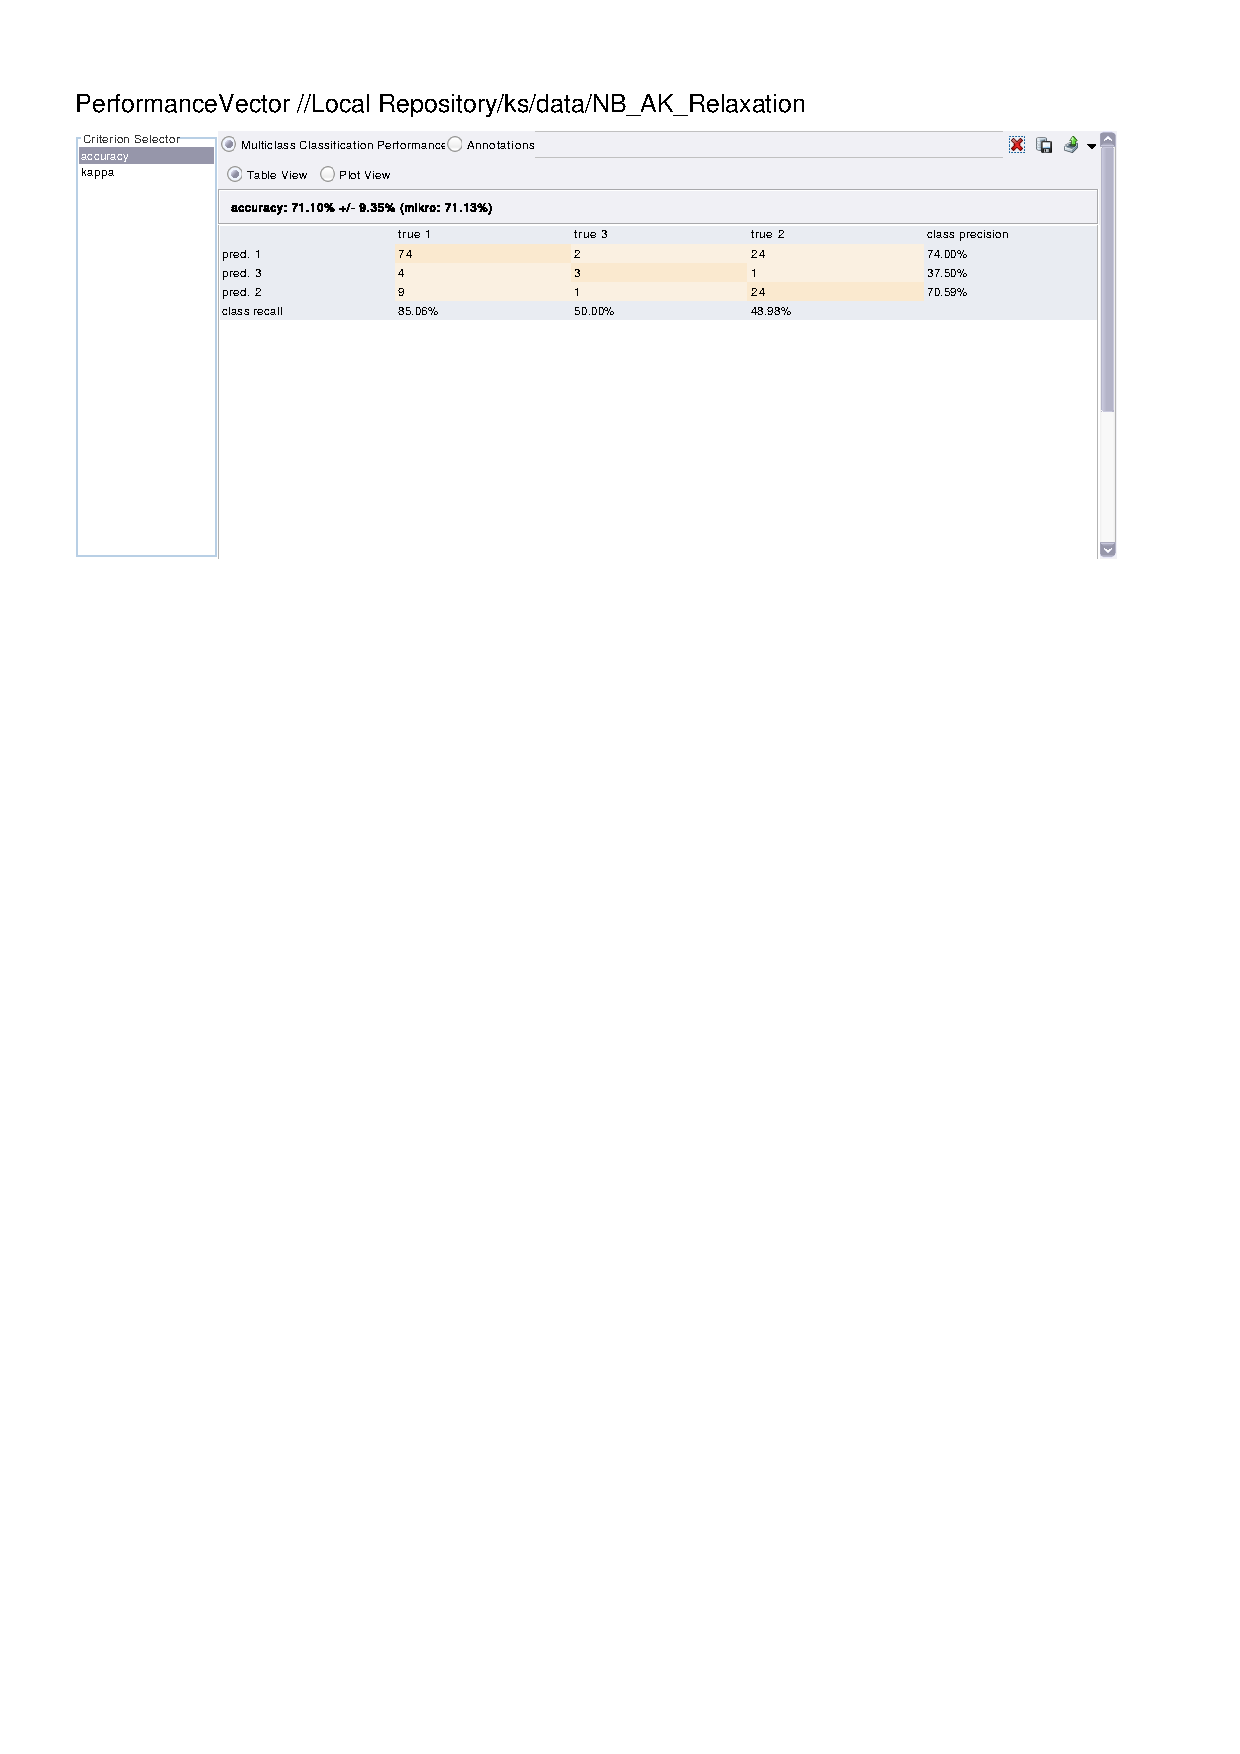
\includegraphics[trim=0 680 0 60,clip,width=16.09cm]{results/NB_A_Relaxation.pdf}} \caption{
} \label{NB_K_Relaxation}
\end{figure}

\begin{figure}[htp]
  \centerline{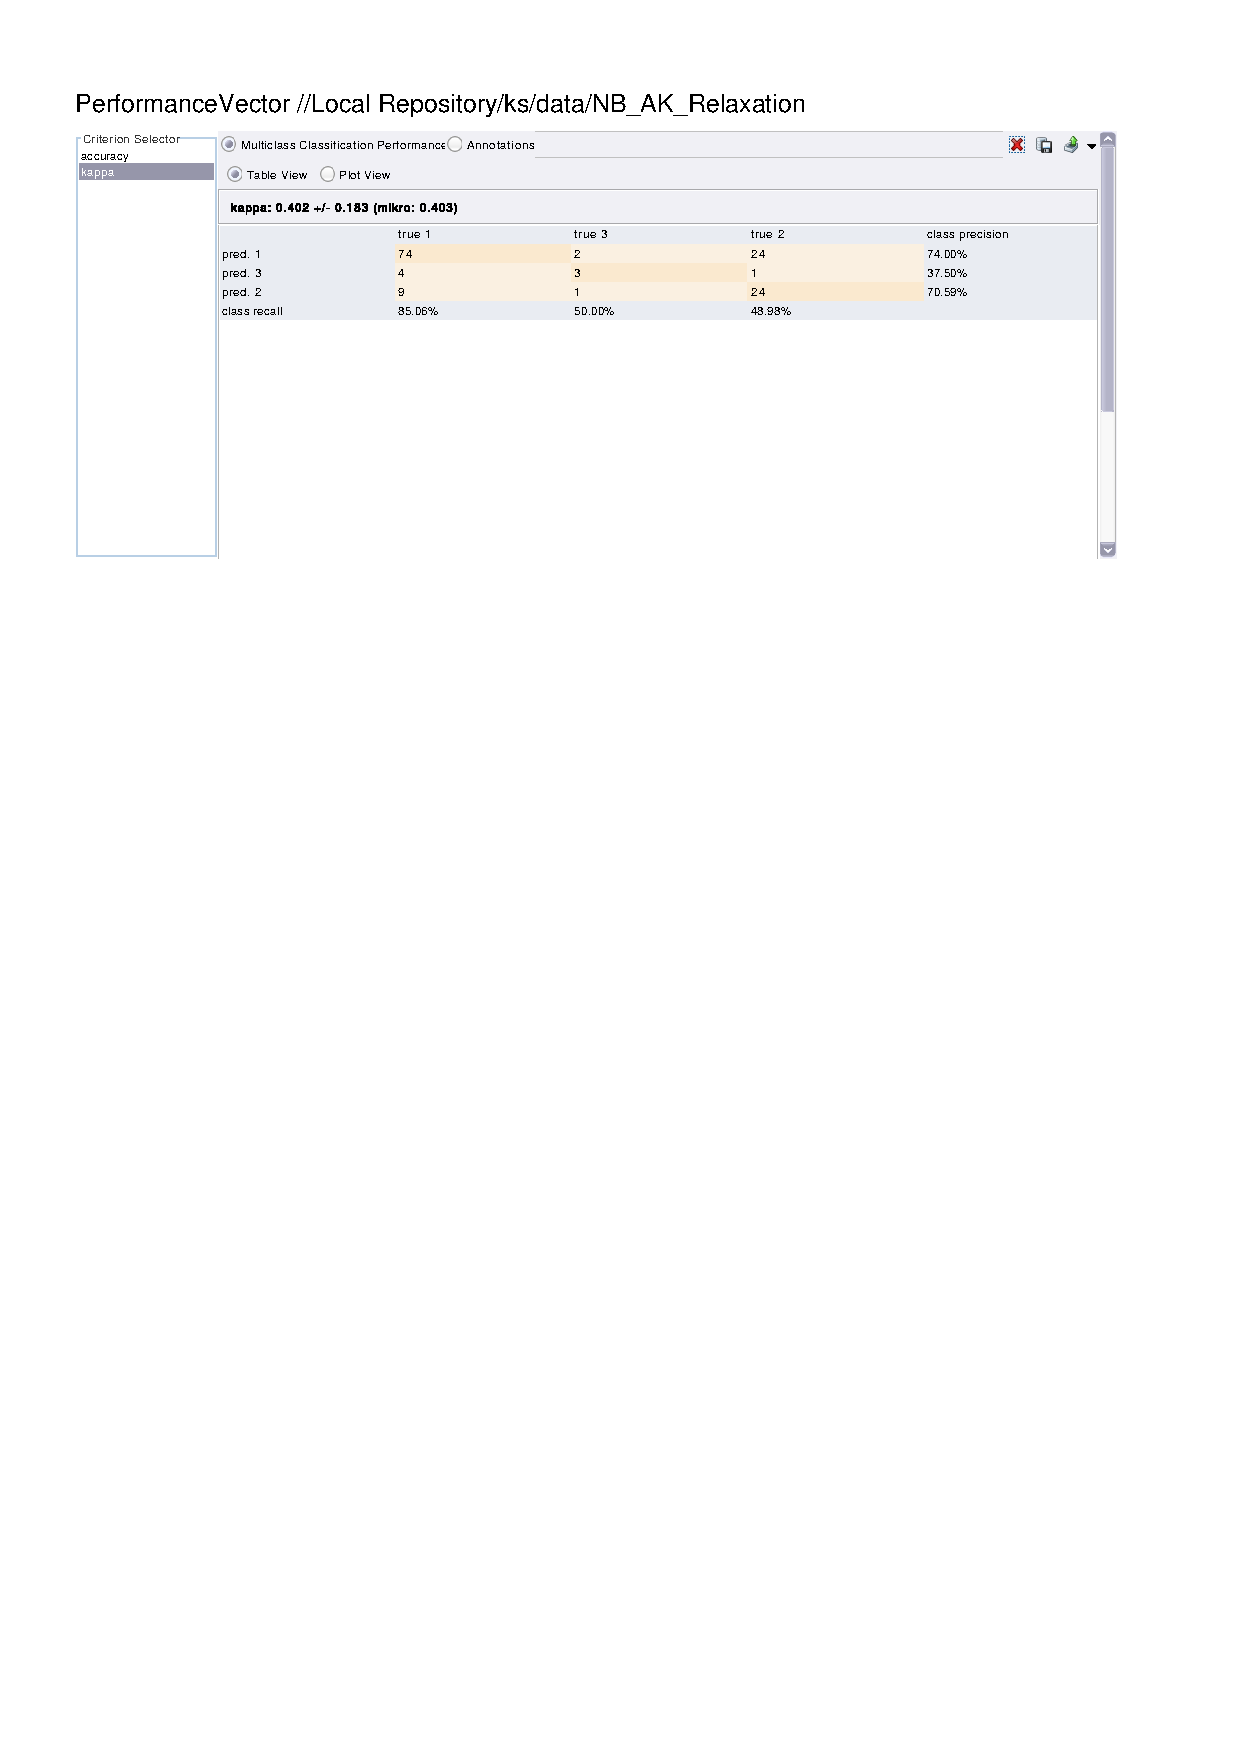
\includegraphics[trim=0 680 0 60,clip,width=16.09cm]{results/NB_K_Relaxation.pdf}} \caption{
} \label{NB_K_Relaxation}
\end{figure}

\clearpage
\FloatBarrier
\subsection{Árboles de Decisión}
\subsubsection{Aburrimiento}

% J48 Boredom

\begin{figure}[htp]
  \centerline{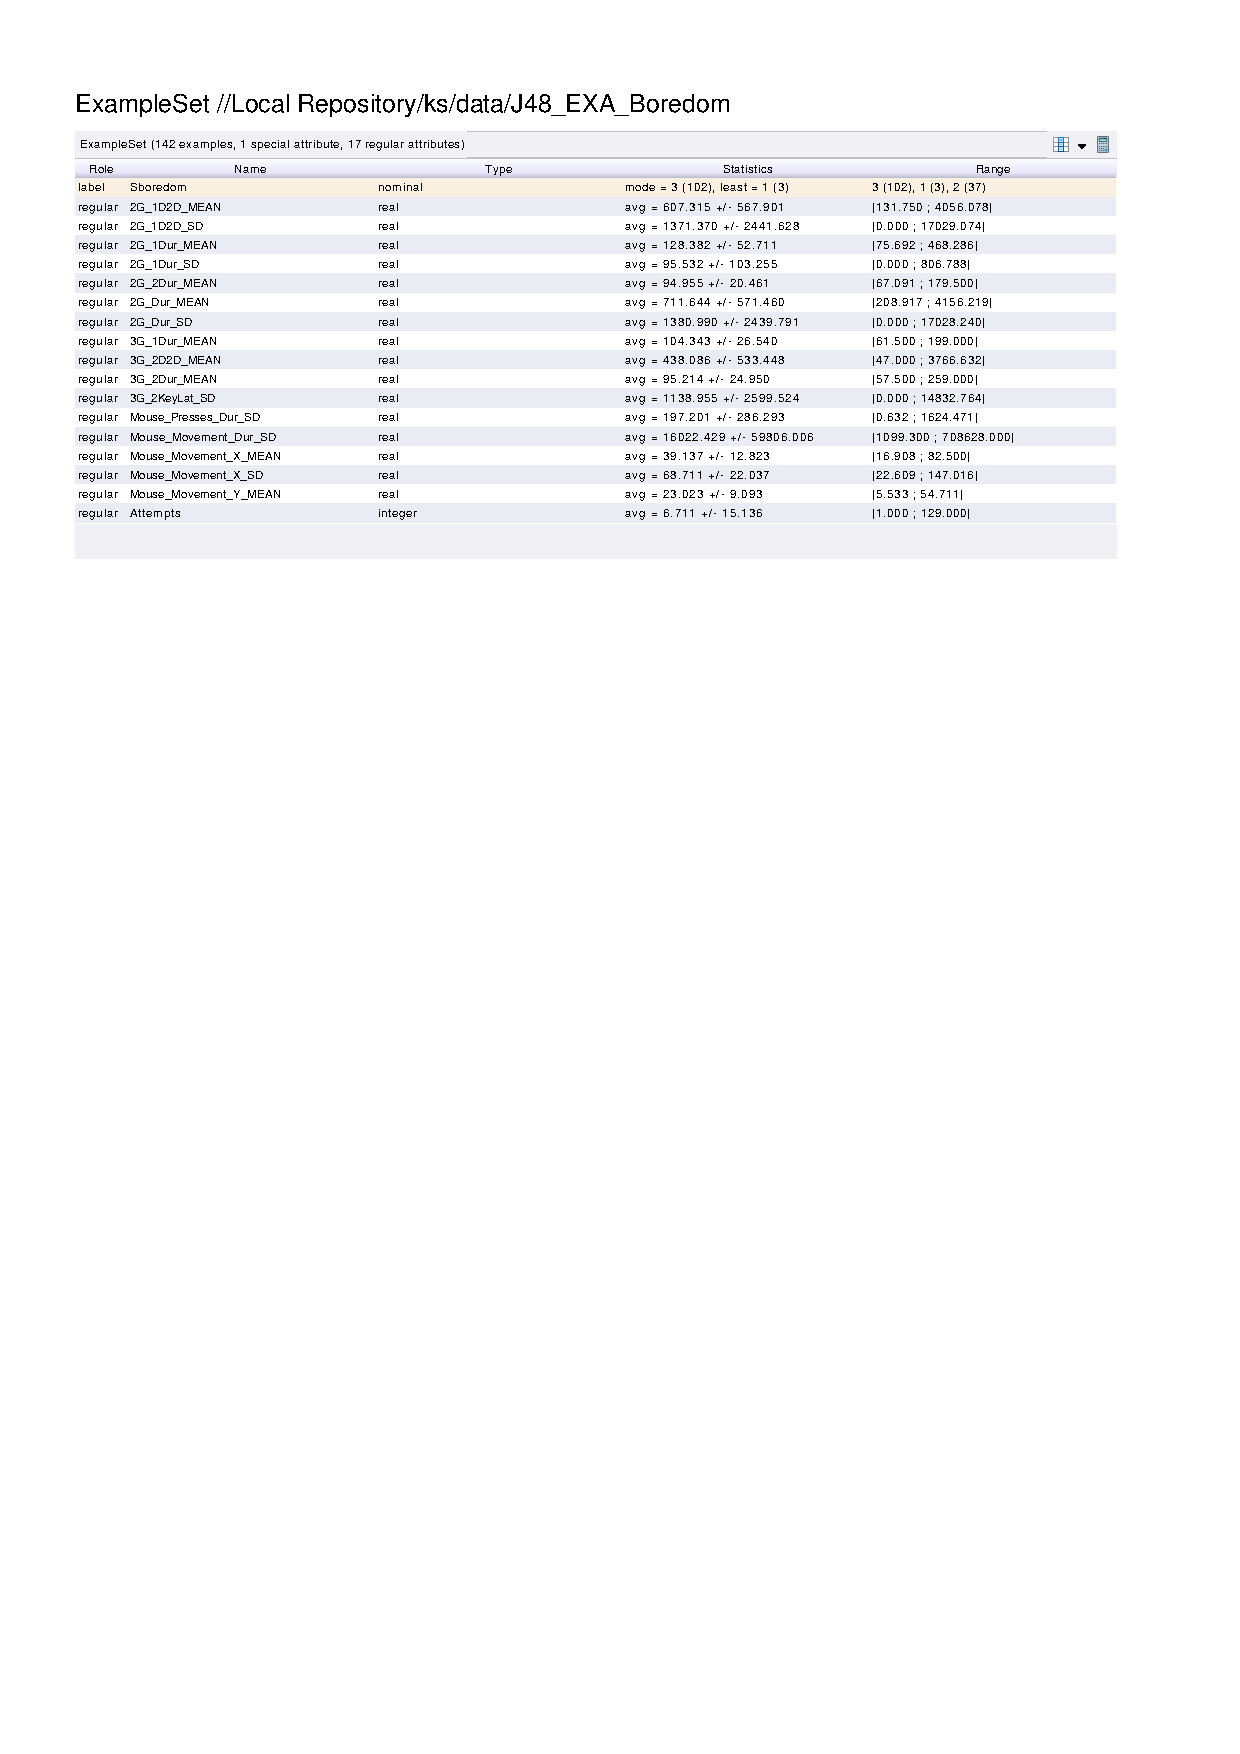
\includegraphics[trim=0 580 0 60,clip,width=16.09cm]{results/J48_EXA_Boredom.pdf}} \caption{
} \label{J48_EXA_Boredom}
\end{figure}

\begin{figure}[htp]
  \centerline{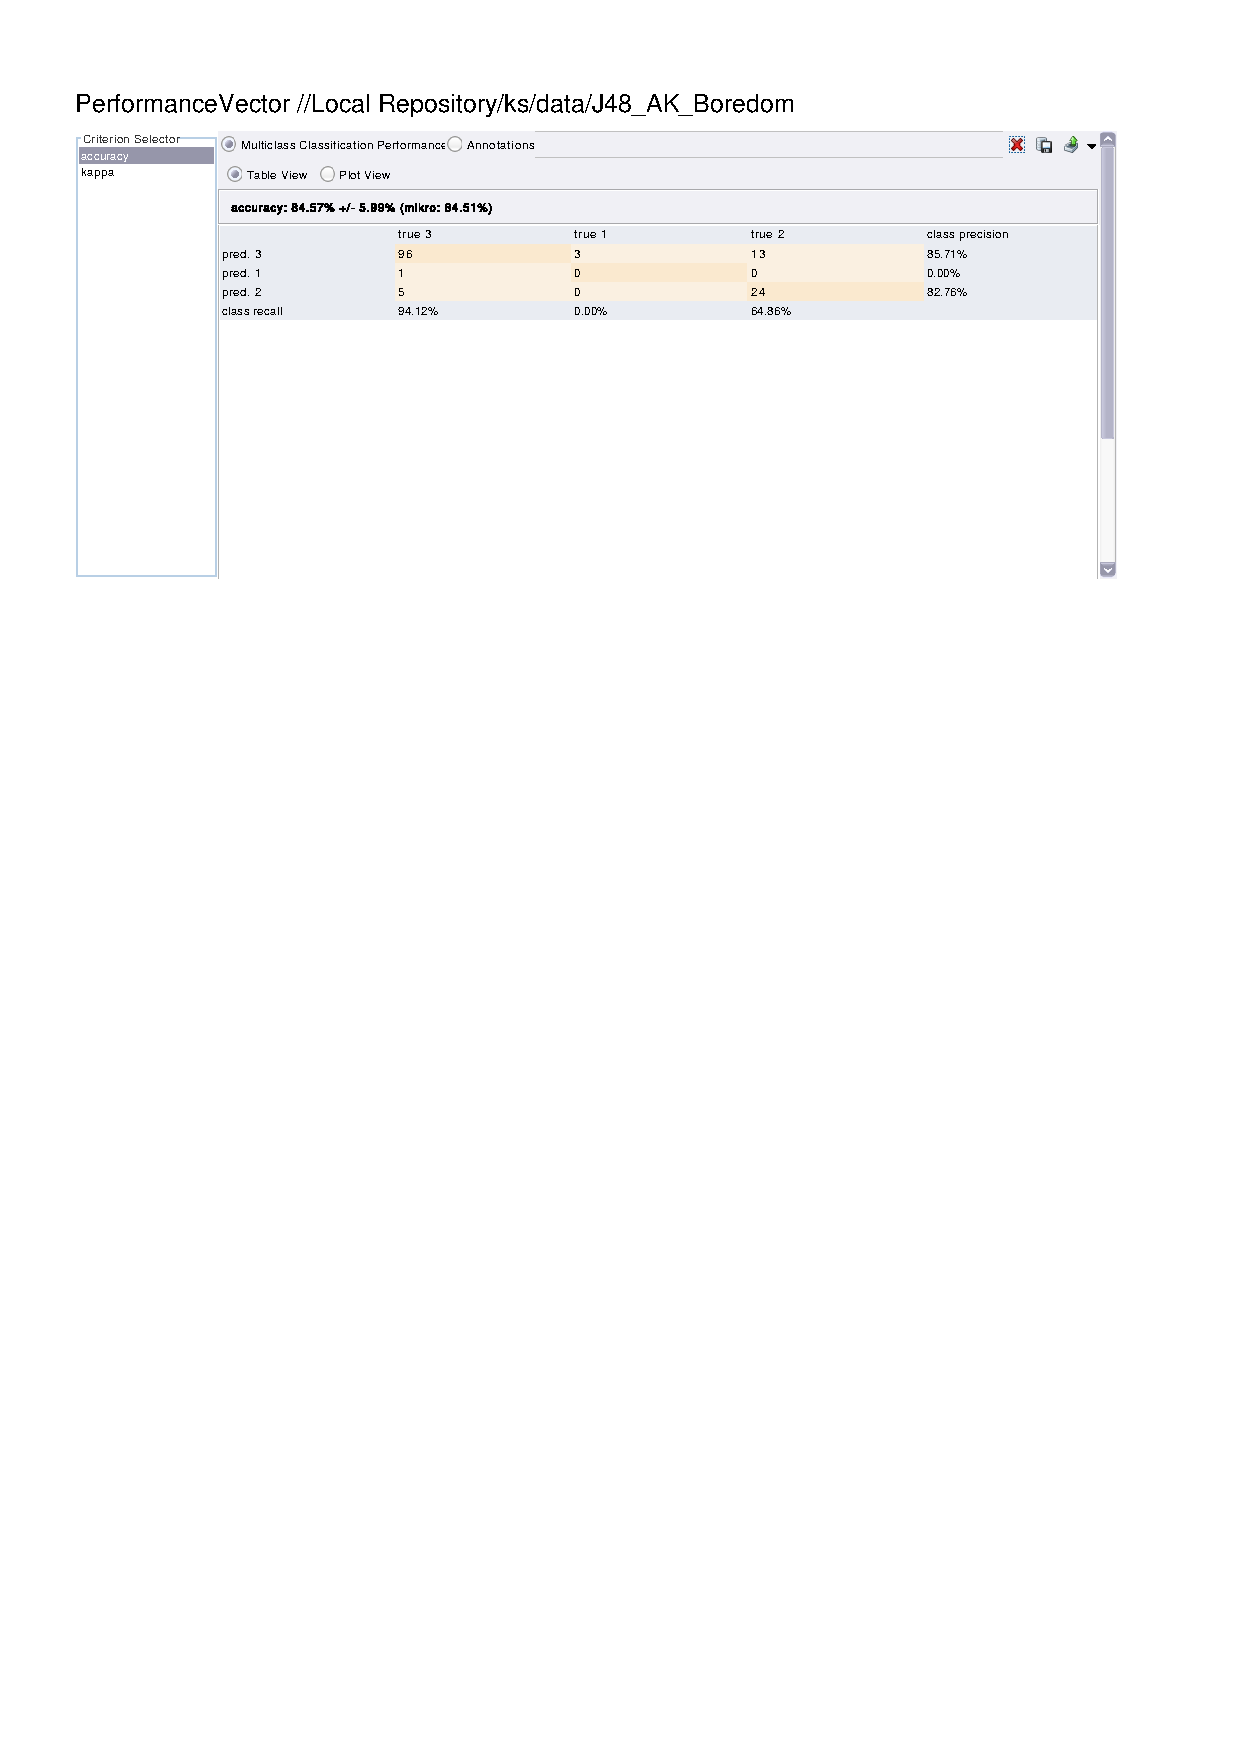
\includegraphics[trim=0 680 0 60,clip,width=16.09cm]{results/J48_A_Boredom.pdf}} \caption{
} \label{J48_A_Boredom}
\end{figure}

\begin{figure}[htp]
  \centerline{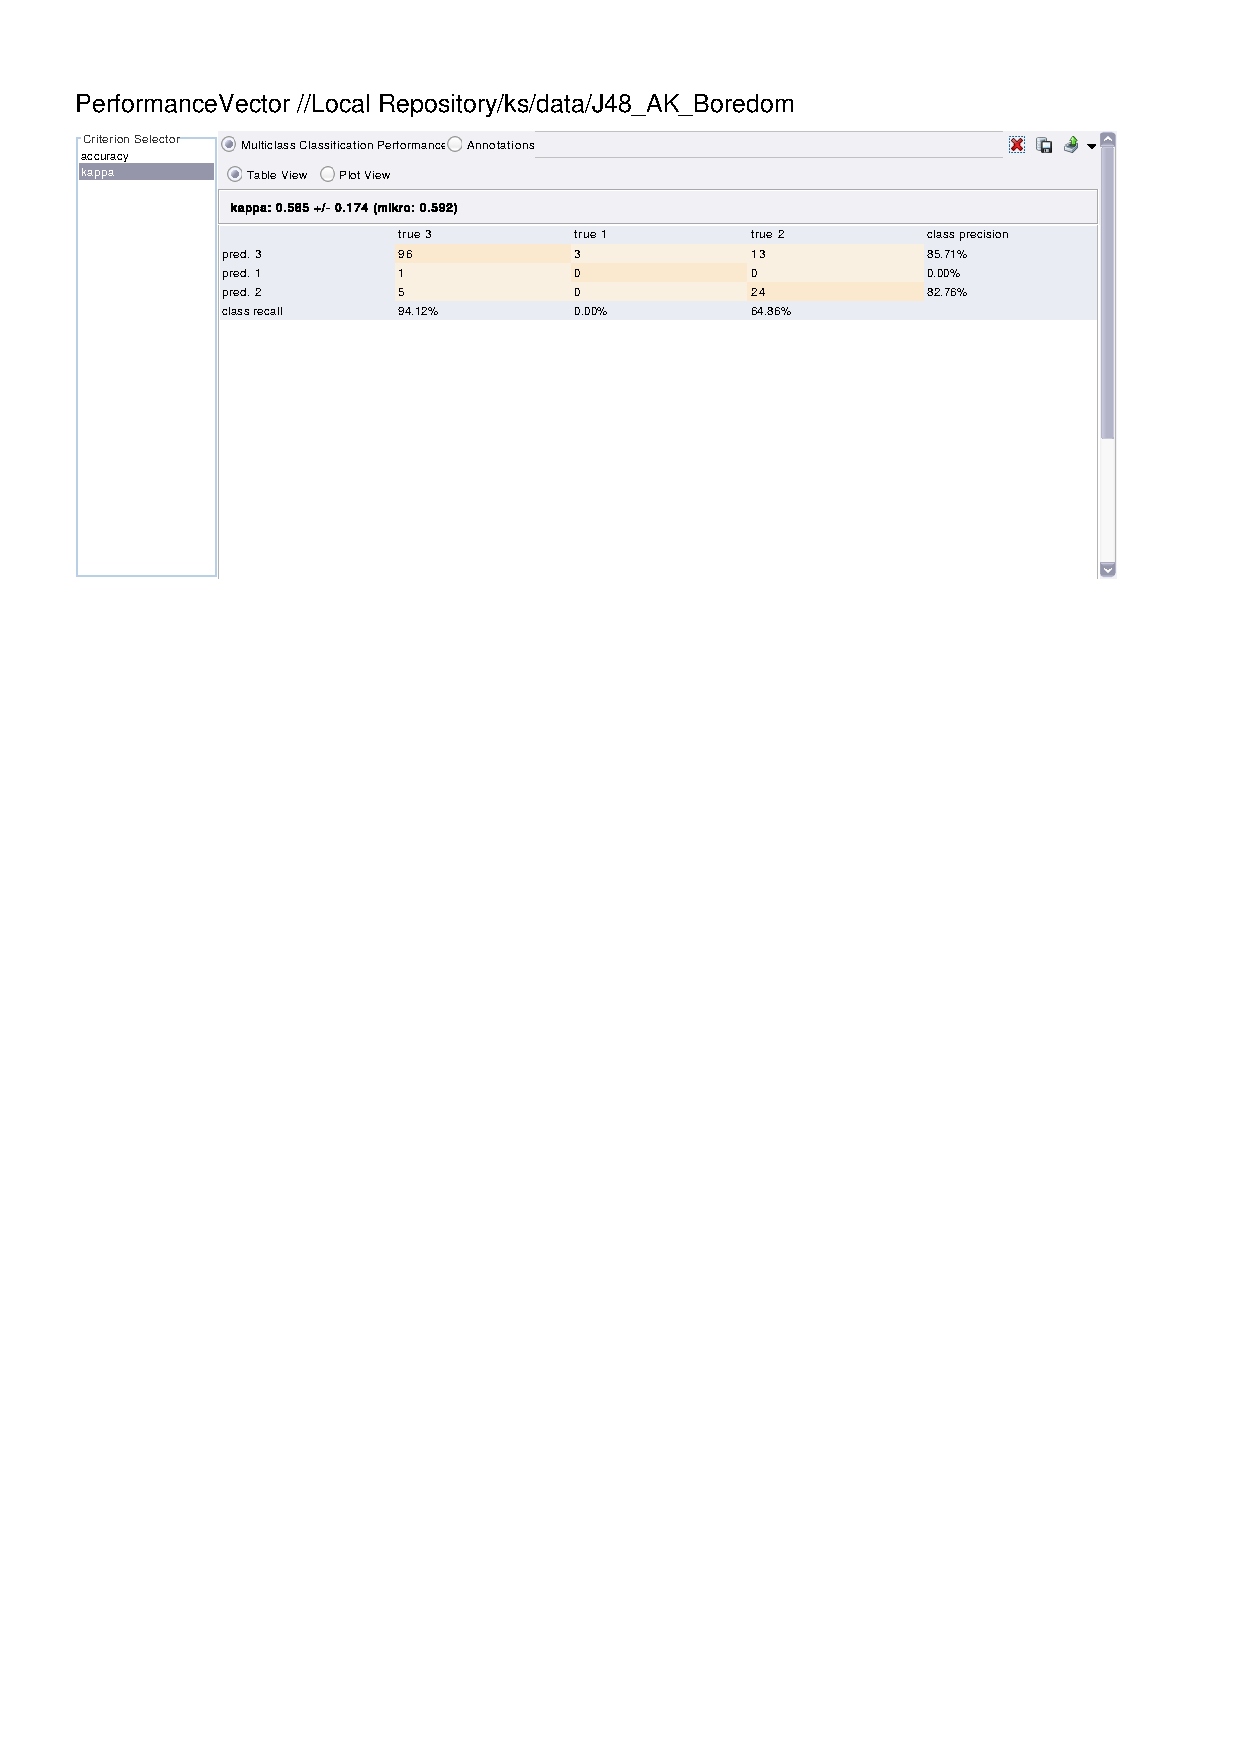
\includegraphics[trim=0 680 0 60,clip,width=16.09cm]{results/J48_K_Boredom.pdf}} \caption{
} \label{J48_K_Boredom}
\end{figure}

\clearpage
\FloatBarrier
% J48 Distraction
\subsubsection{Distracción}

\begin{figure}[htp]
  \centerline{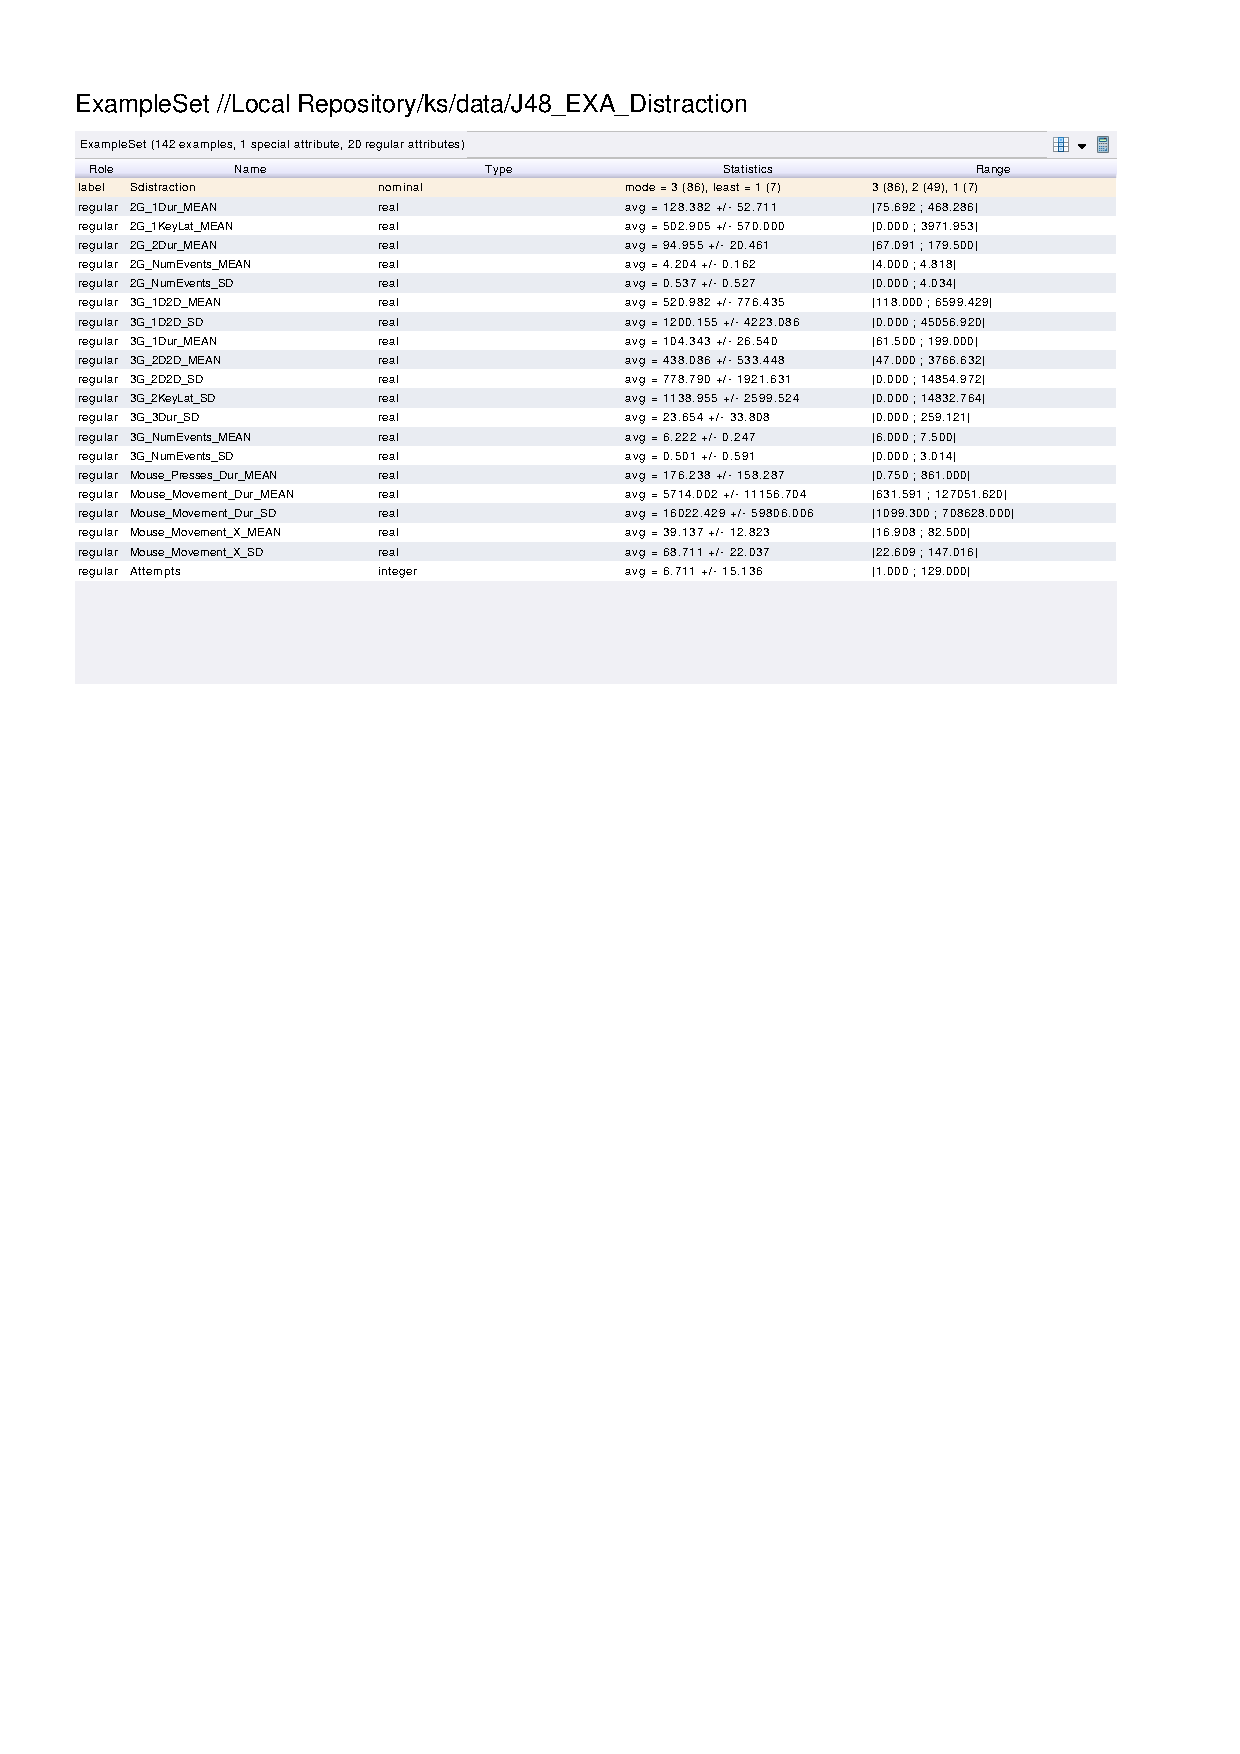
\includegraphics[trim=0 561 0 60,clip,width=16.09cm]{results/J48_EXA_Distraction.pdf}} \caption{
} \label{J48_EXA_Distraction}
\end{figure}

\begin{figure}[htp]
  \centerline{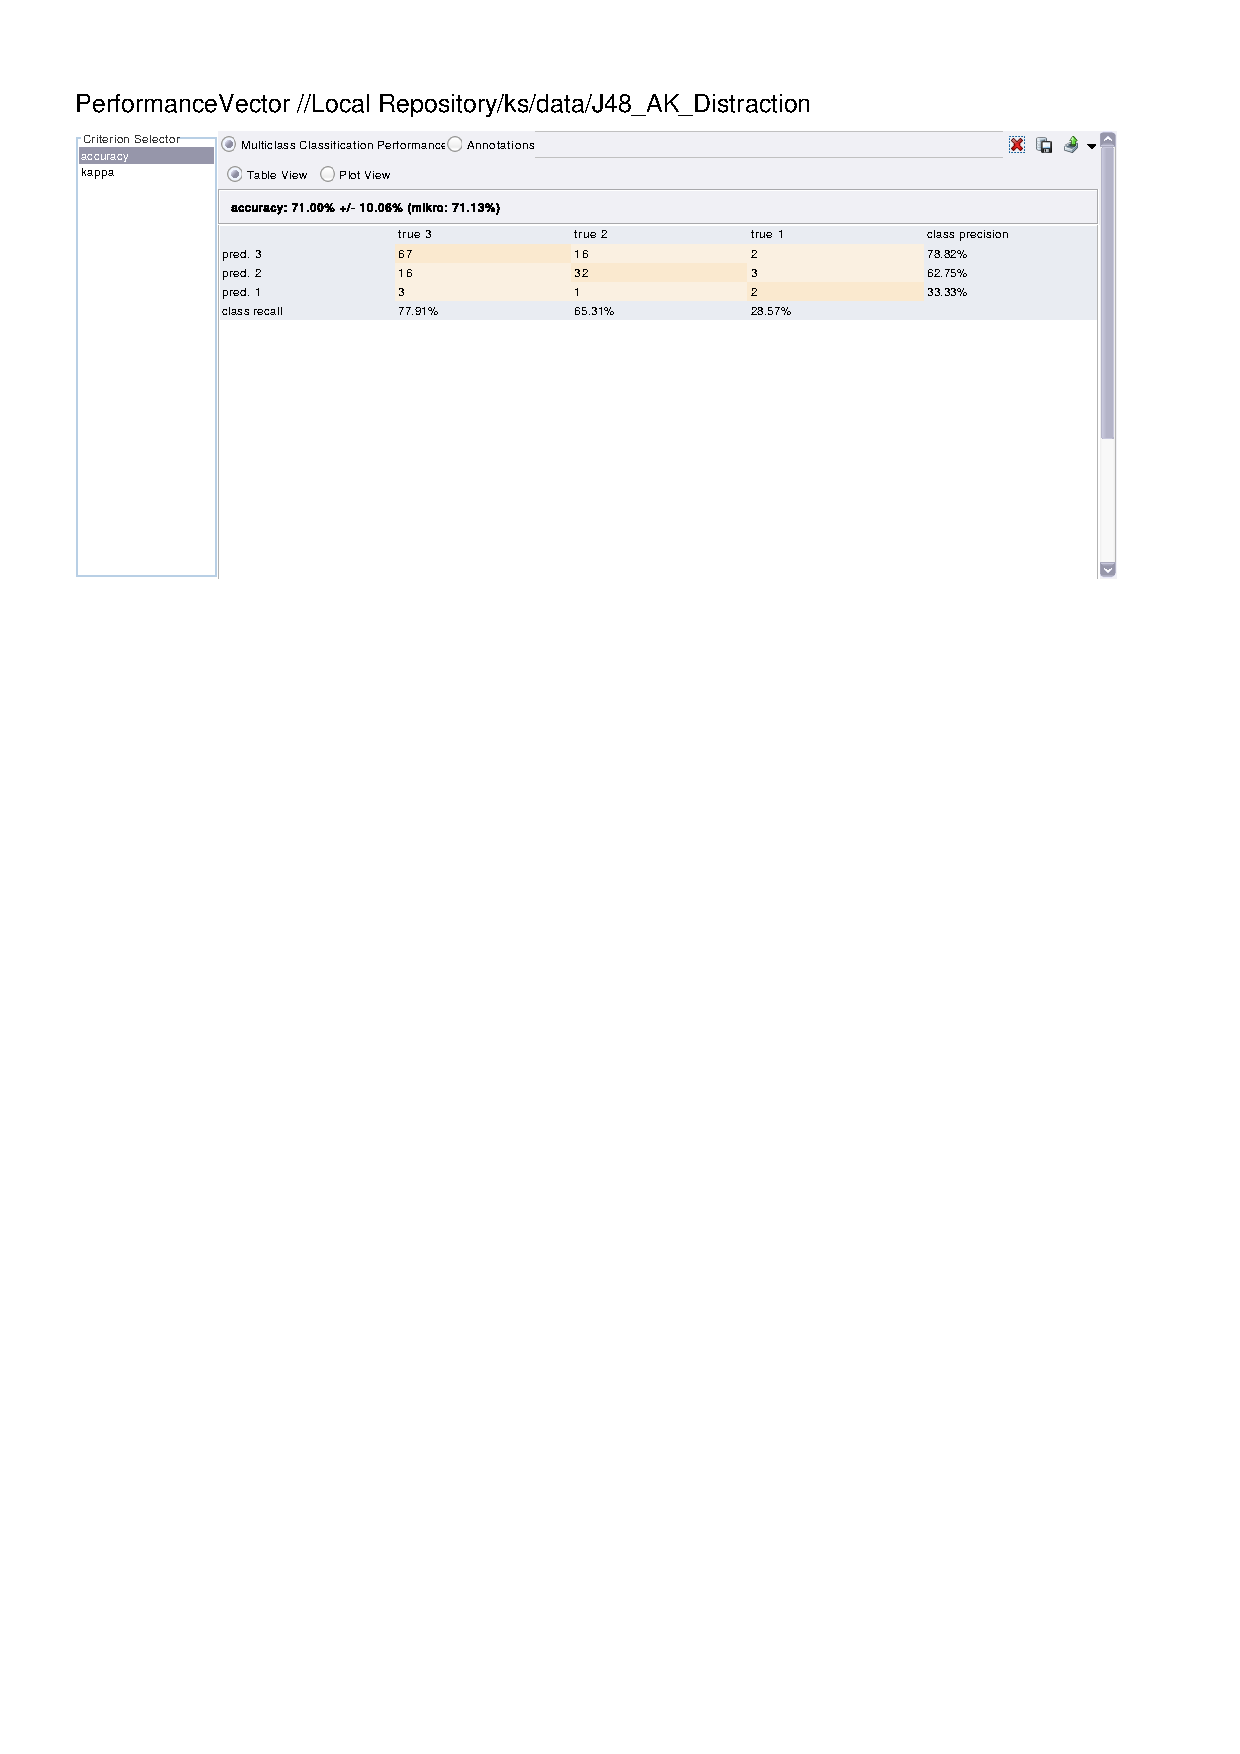
\includegraphics[trim=0 682 0 60,clip,width=16.09cm]{results/J48_A_Distraction.pdf}} \caption{
} \label{J48_A_Distraction}
\end{figure}

\begin{figure}[htp]
  \centerline{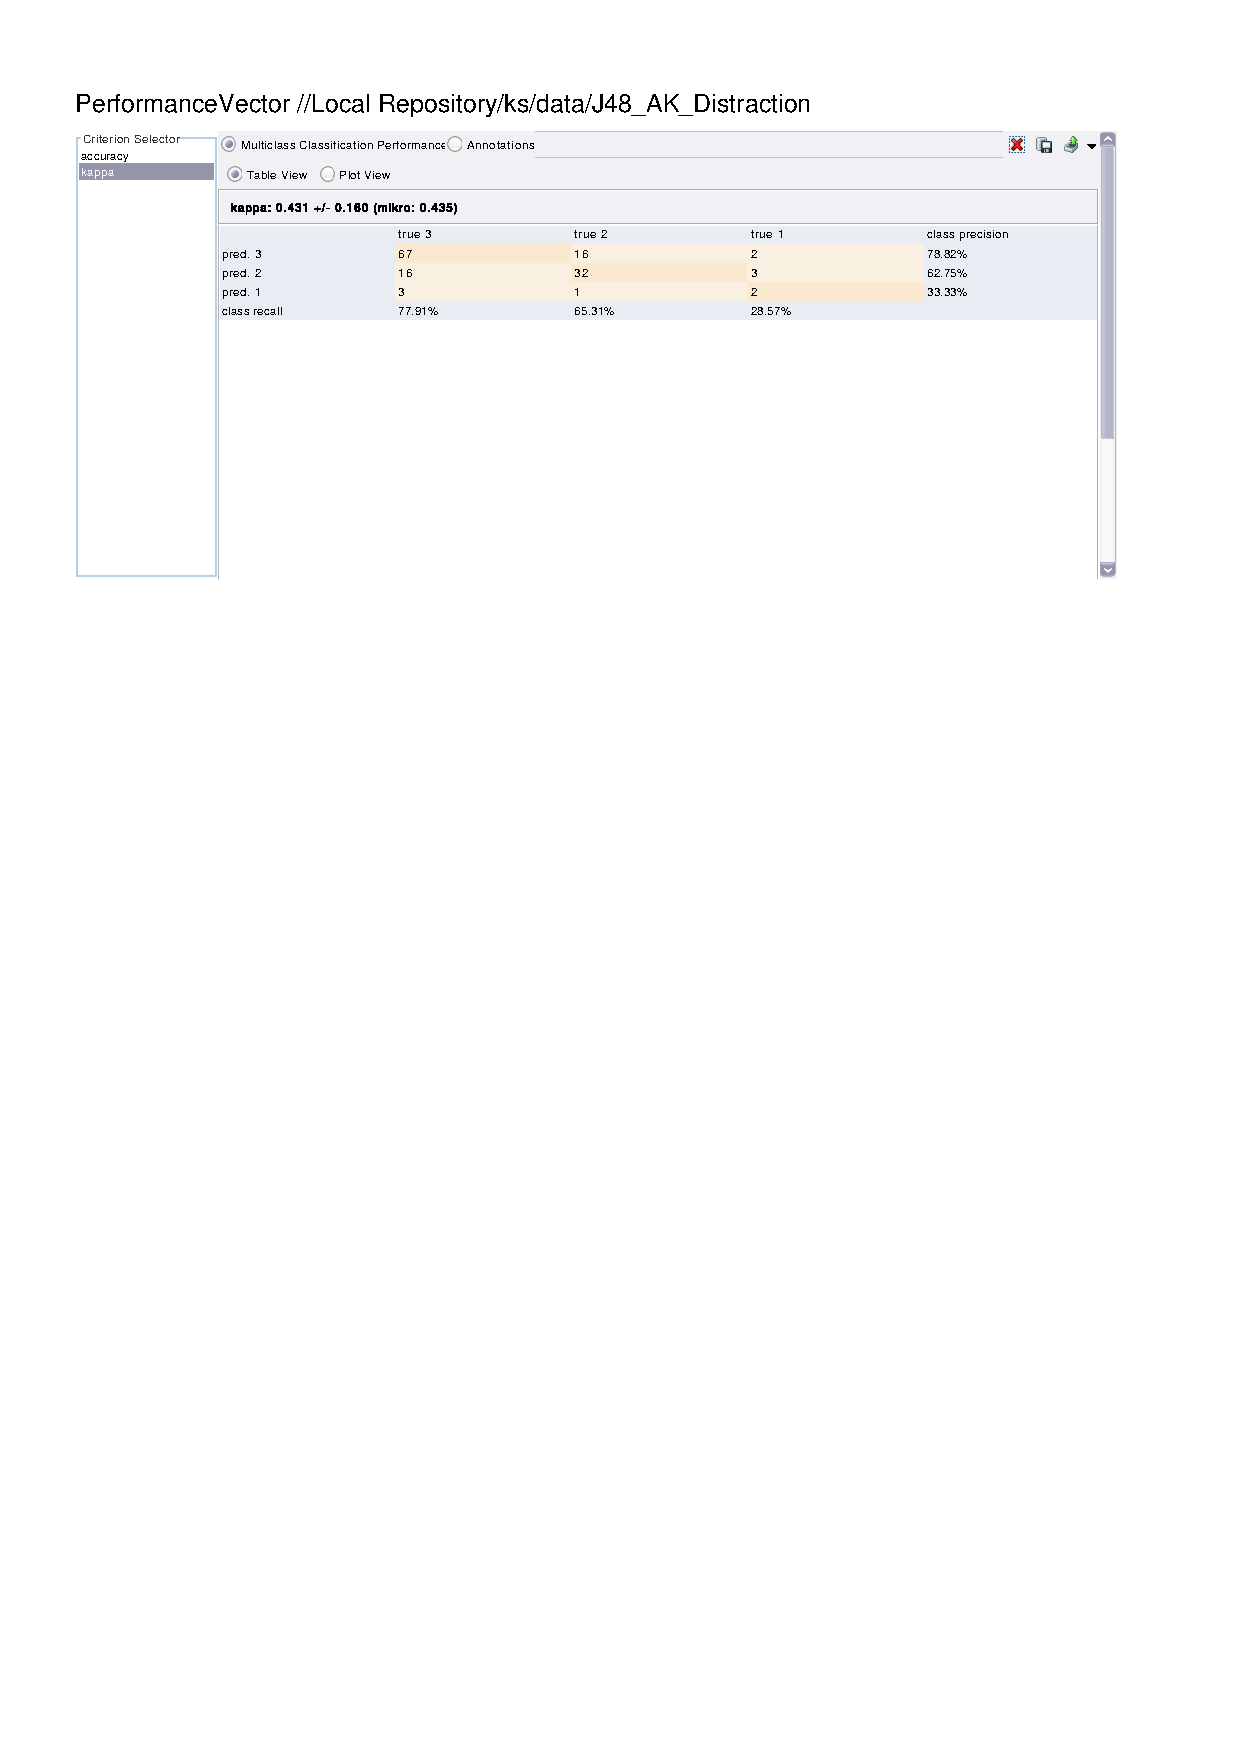
\includegraphics[trim=0 682 0 60,clip,width=16.09cm]{results/J48_K_Distraction.pdf}} \caption{
} \label{J48_K_Distraction}
\end{figure}

\clearpage
\FloatBarrier
% J48 Excitement
\subsubsection{Entusiasmo}

\begin{figure}[htp]
  \centerline{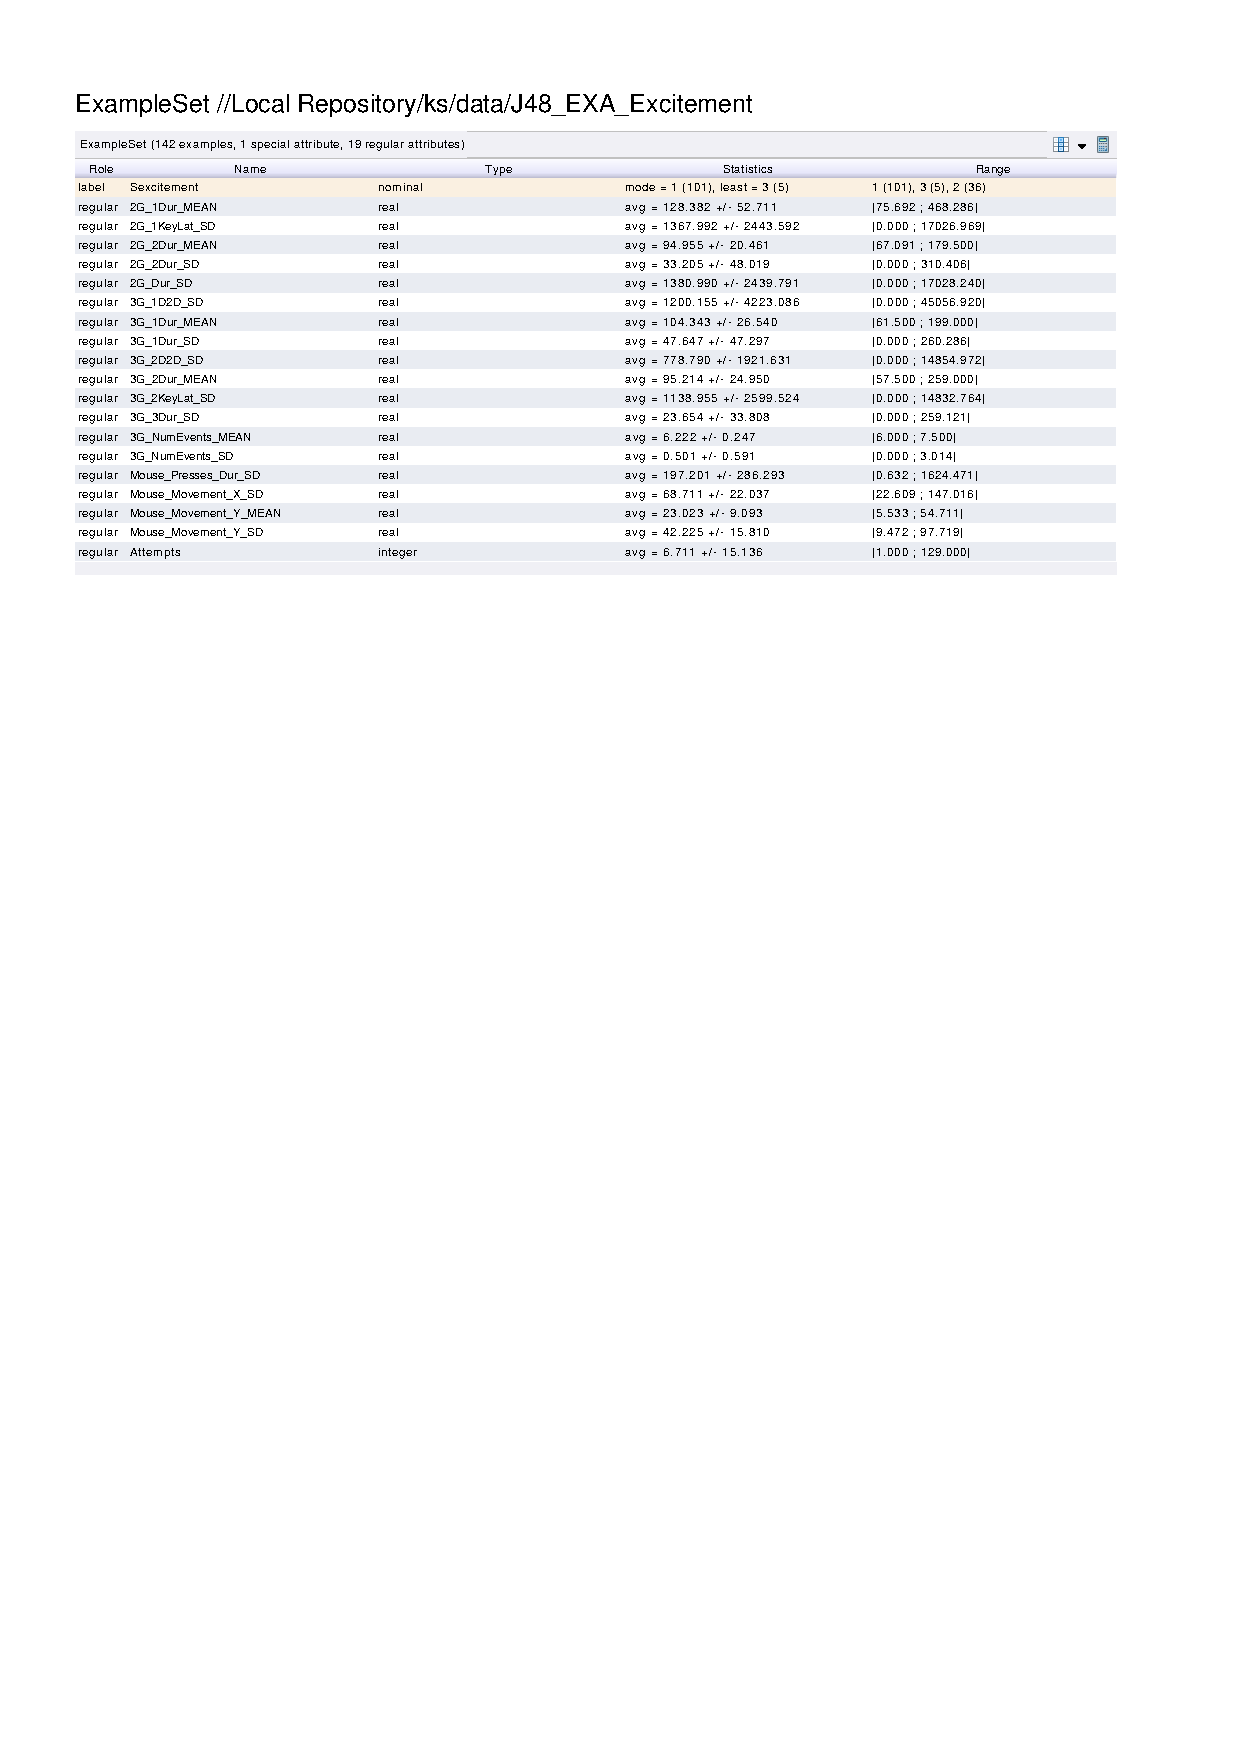
\includegraphics[trim=0 560 0 60,clip,width=16.09cm]{results/J48_EXA_Excitement.pdf}} \caption{
} \label{J48_K_Excitement}
\end{figure}

\begin{figure}[htp]
  \centerline{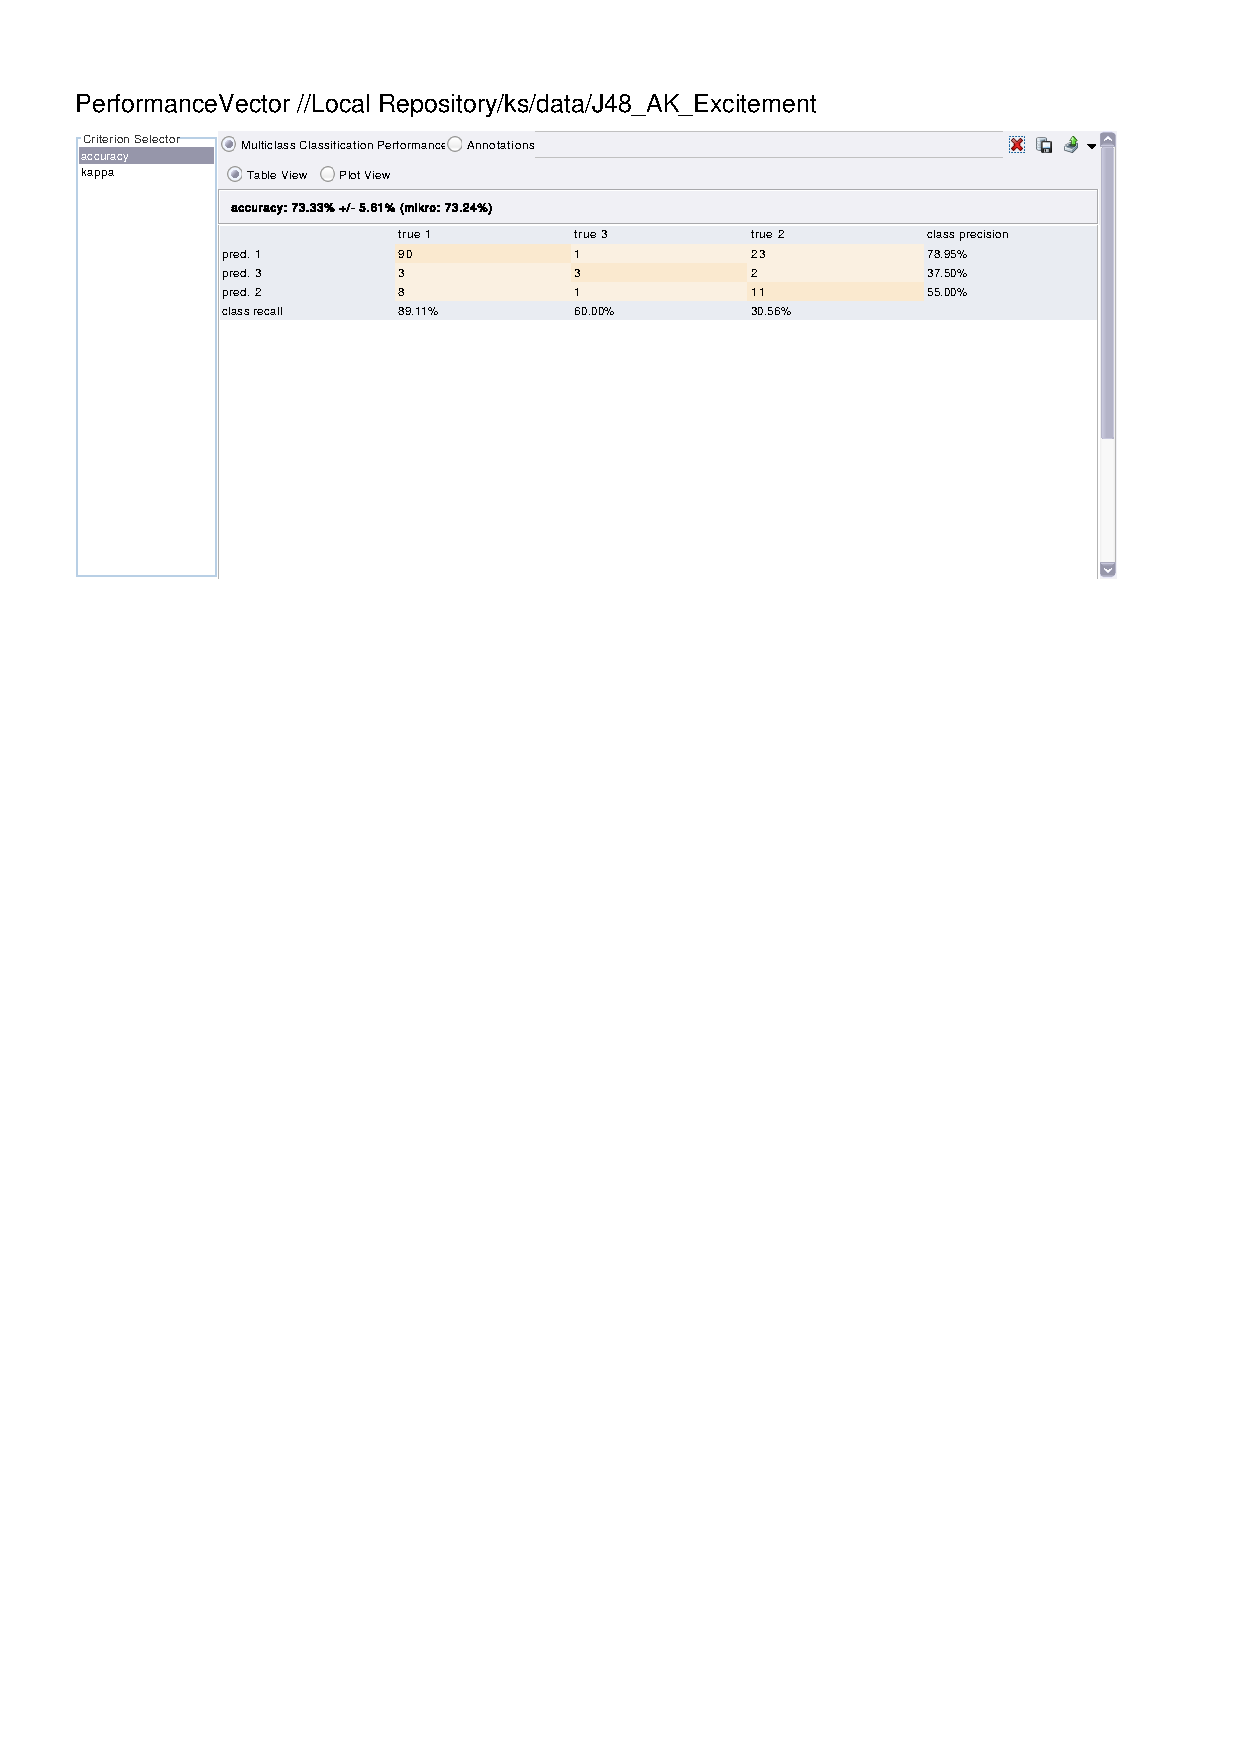
\includegraphics[trim=0 683 0 60,clip,width=16.09cm]{results/J48_A_Excitement.pdf}} \caption{
} \label{J48_K_Excitement}
\end{figure}

\begin{figure}[htp]
  \centerline{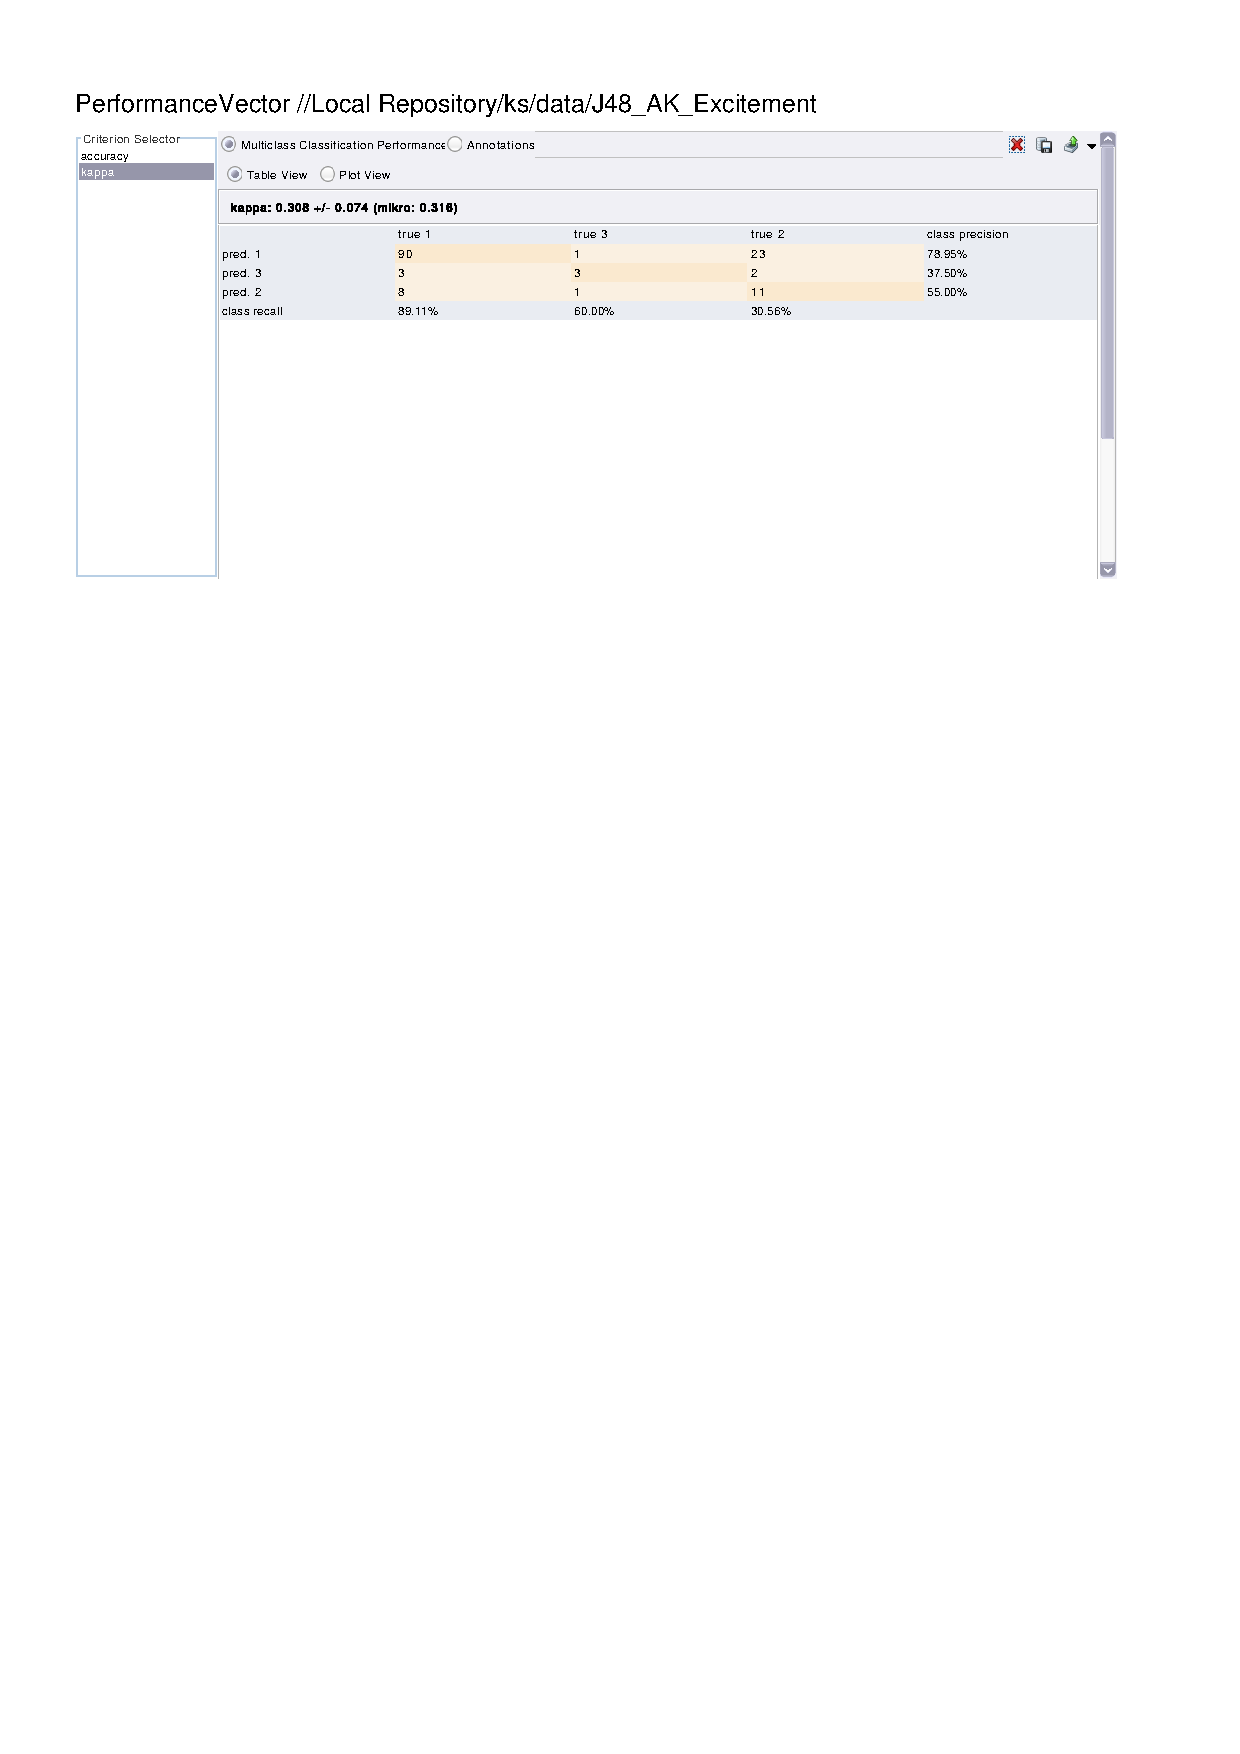
\includegraphics[trim=0 683 0 60,clip,width=16.09cm]{results/J48_K_Excitement.pdf}} \caption{
} \label{J48_K_Excitement}
\end{figure}

\clearpage
\FloatBarrier
% J48 Focus
\subsubsection{Concentración}

\begin{figure}[htp]
  \centerline{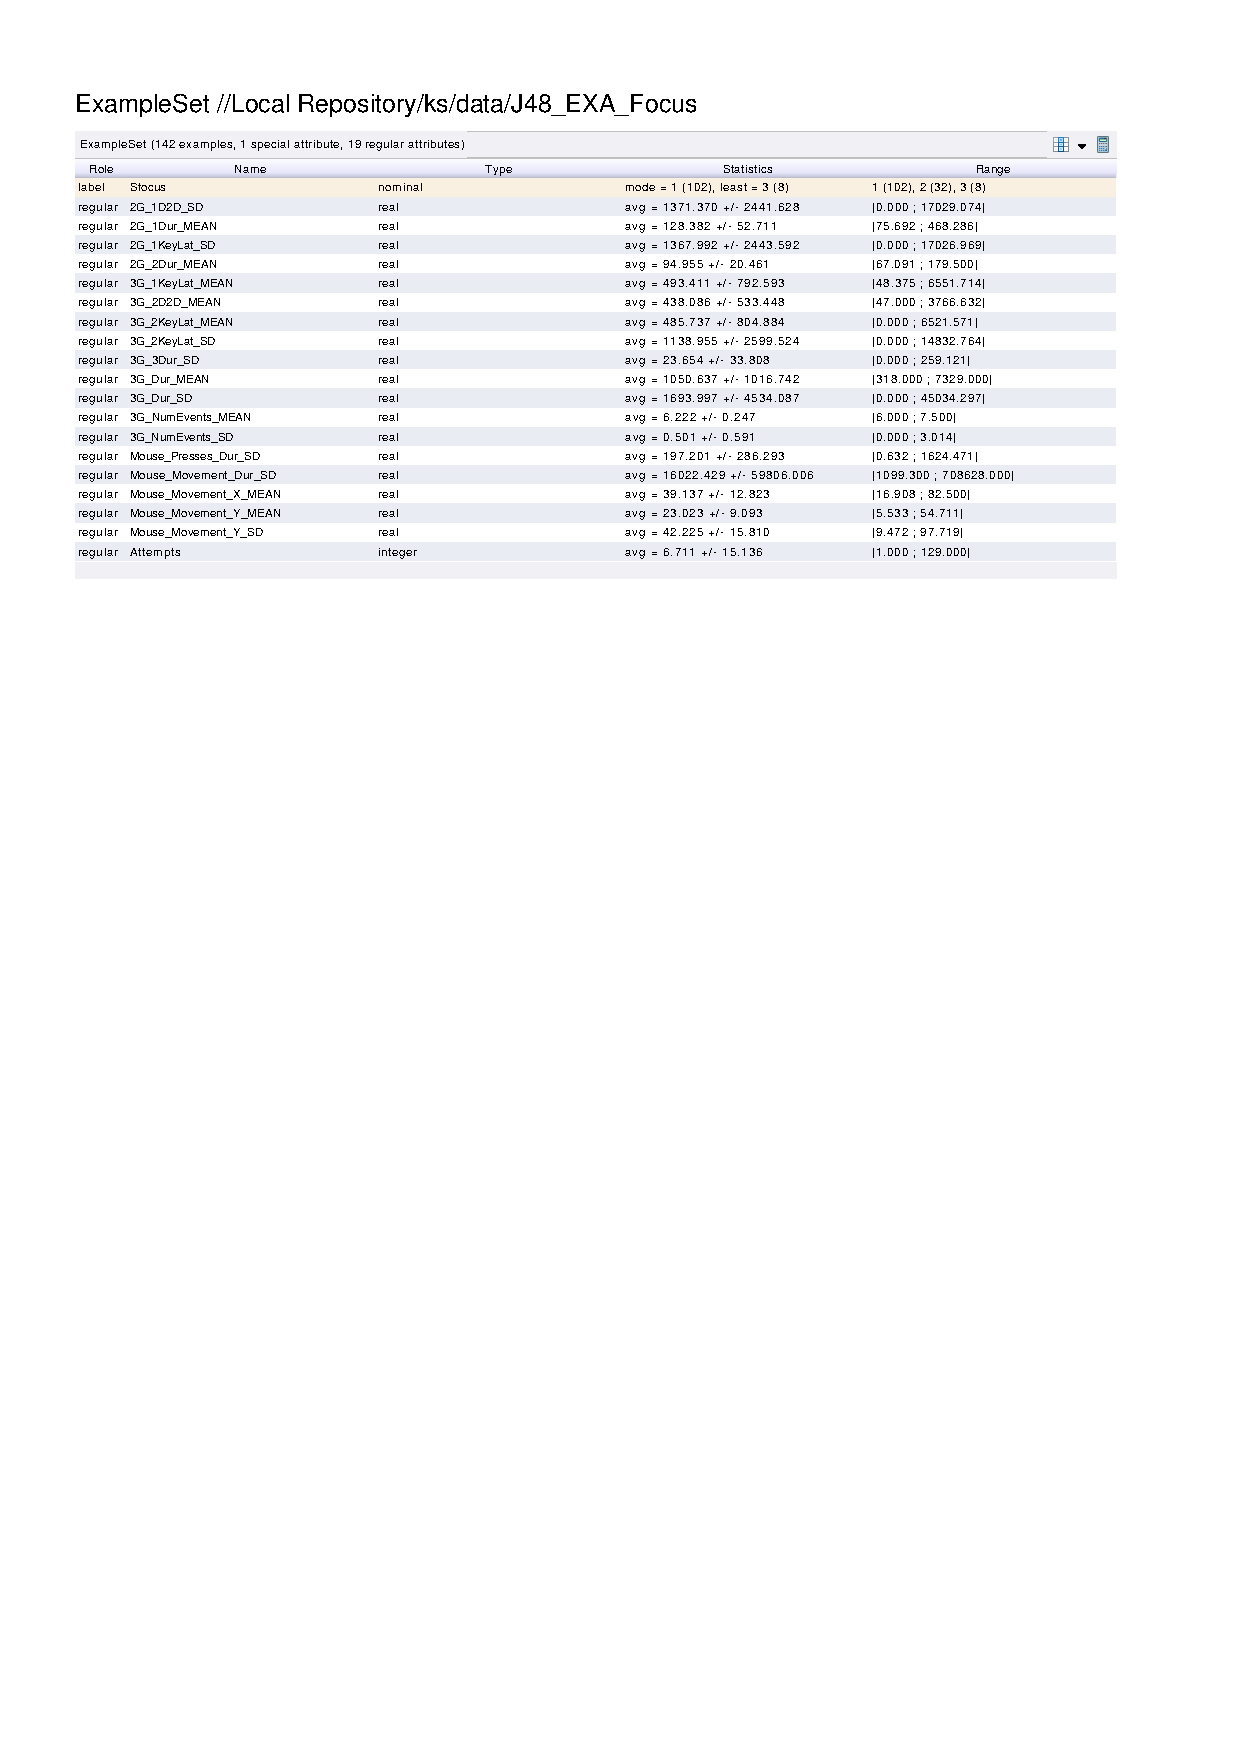
\includegraphics[trim=0 560 0 60,clip,width=16.09cm]{results/J48_EXA_Focus.pdf}} \caption{
} \label{J48_K_Focus}
\end{figure}

\begin{figure}[htp]
  \centerline{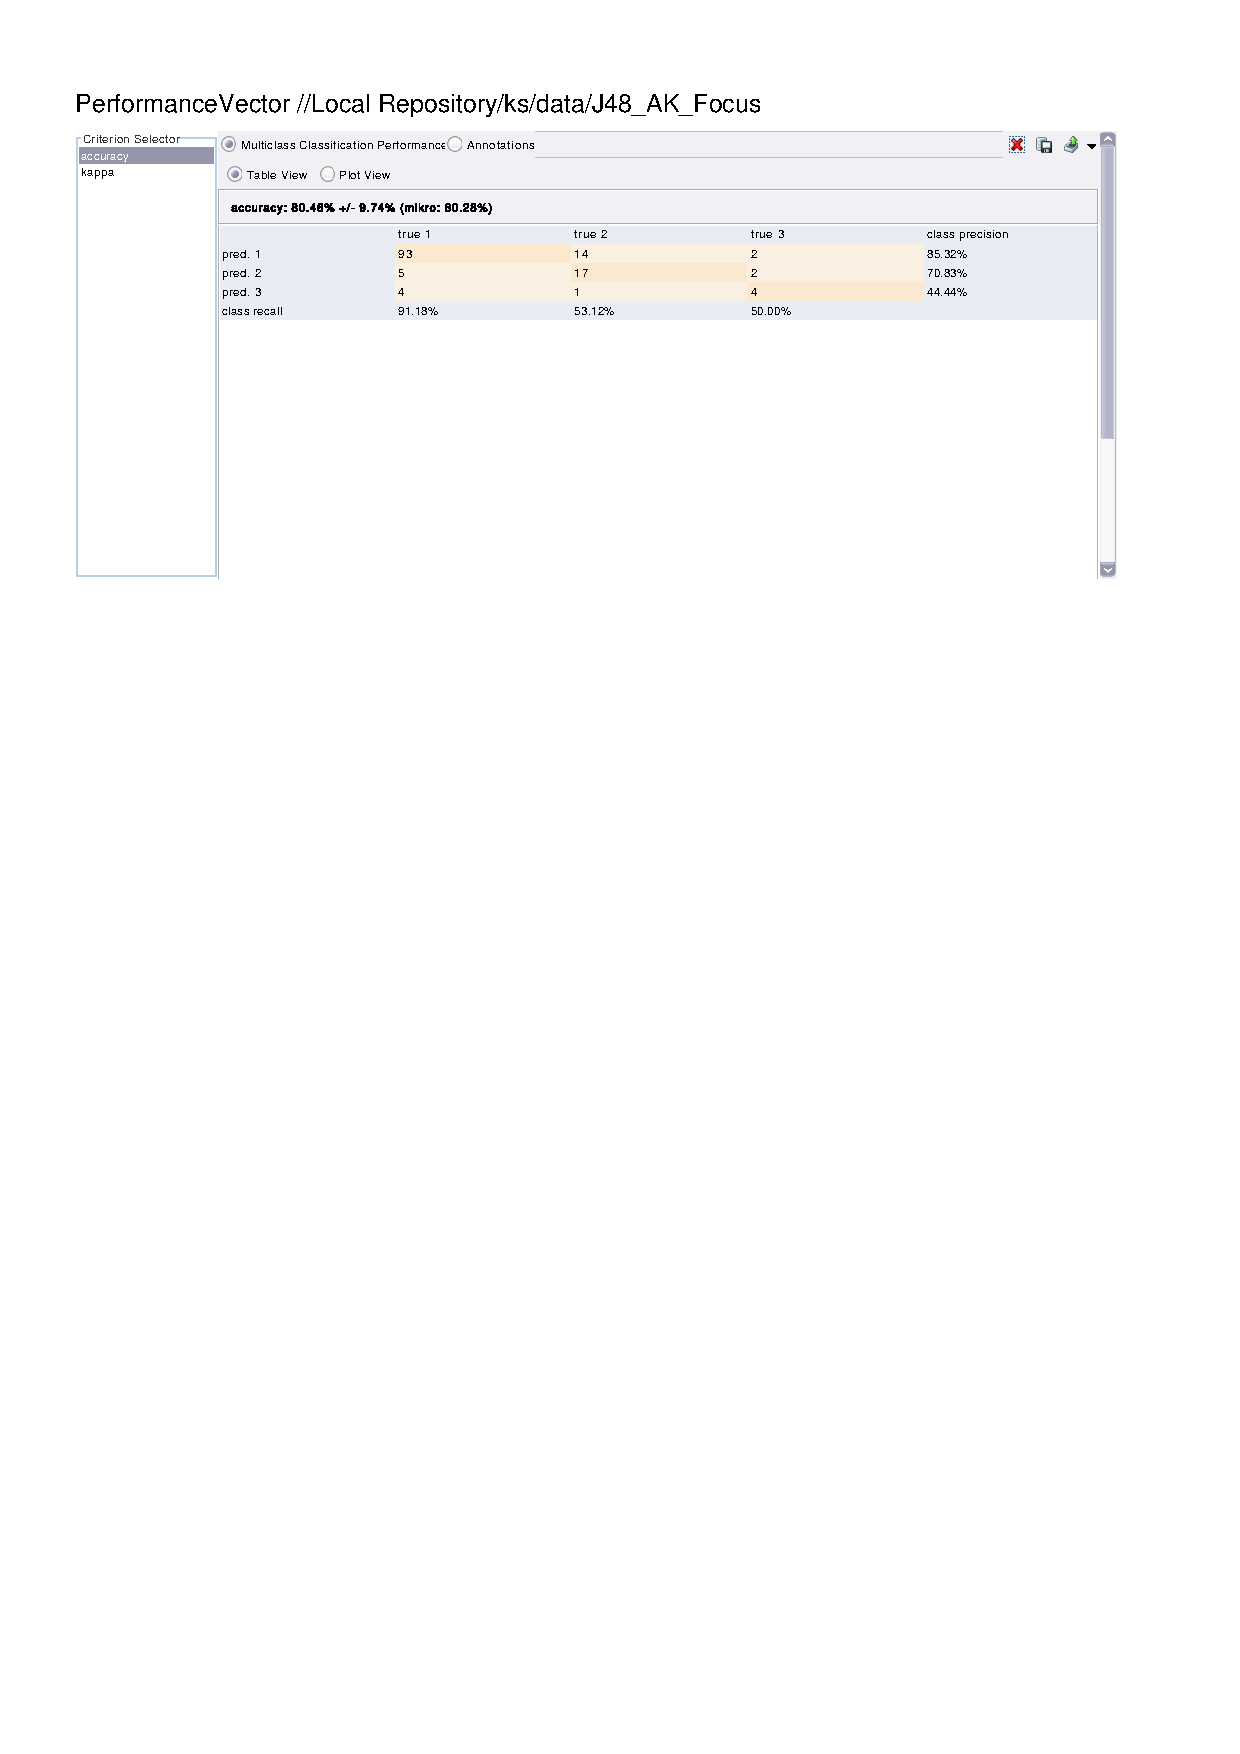
\includegraphics[trim=0 683 0 60,clip,width=16.09cm]{results/J48_A_Focus.pdf}} \caption{
} \label{J48_K_Focus}
\end{figure}

\begin{figure}[htp]
  \centerline{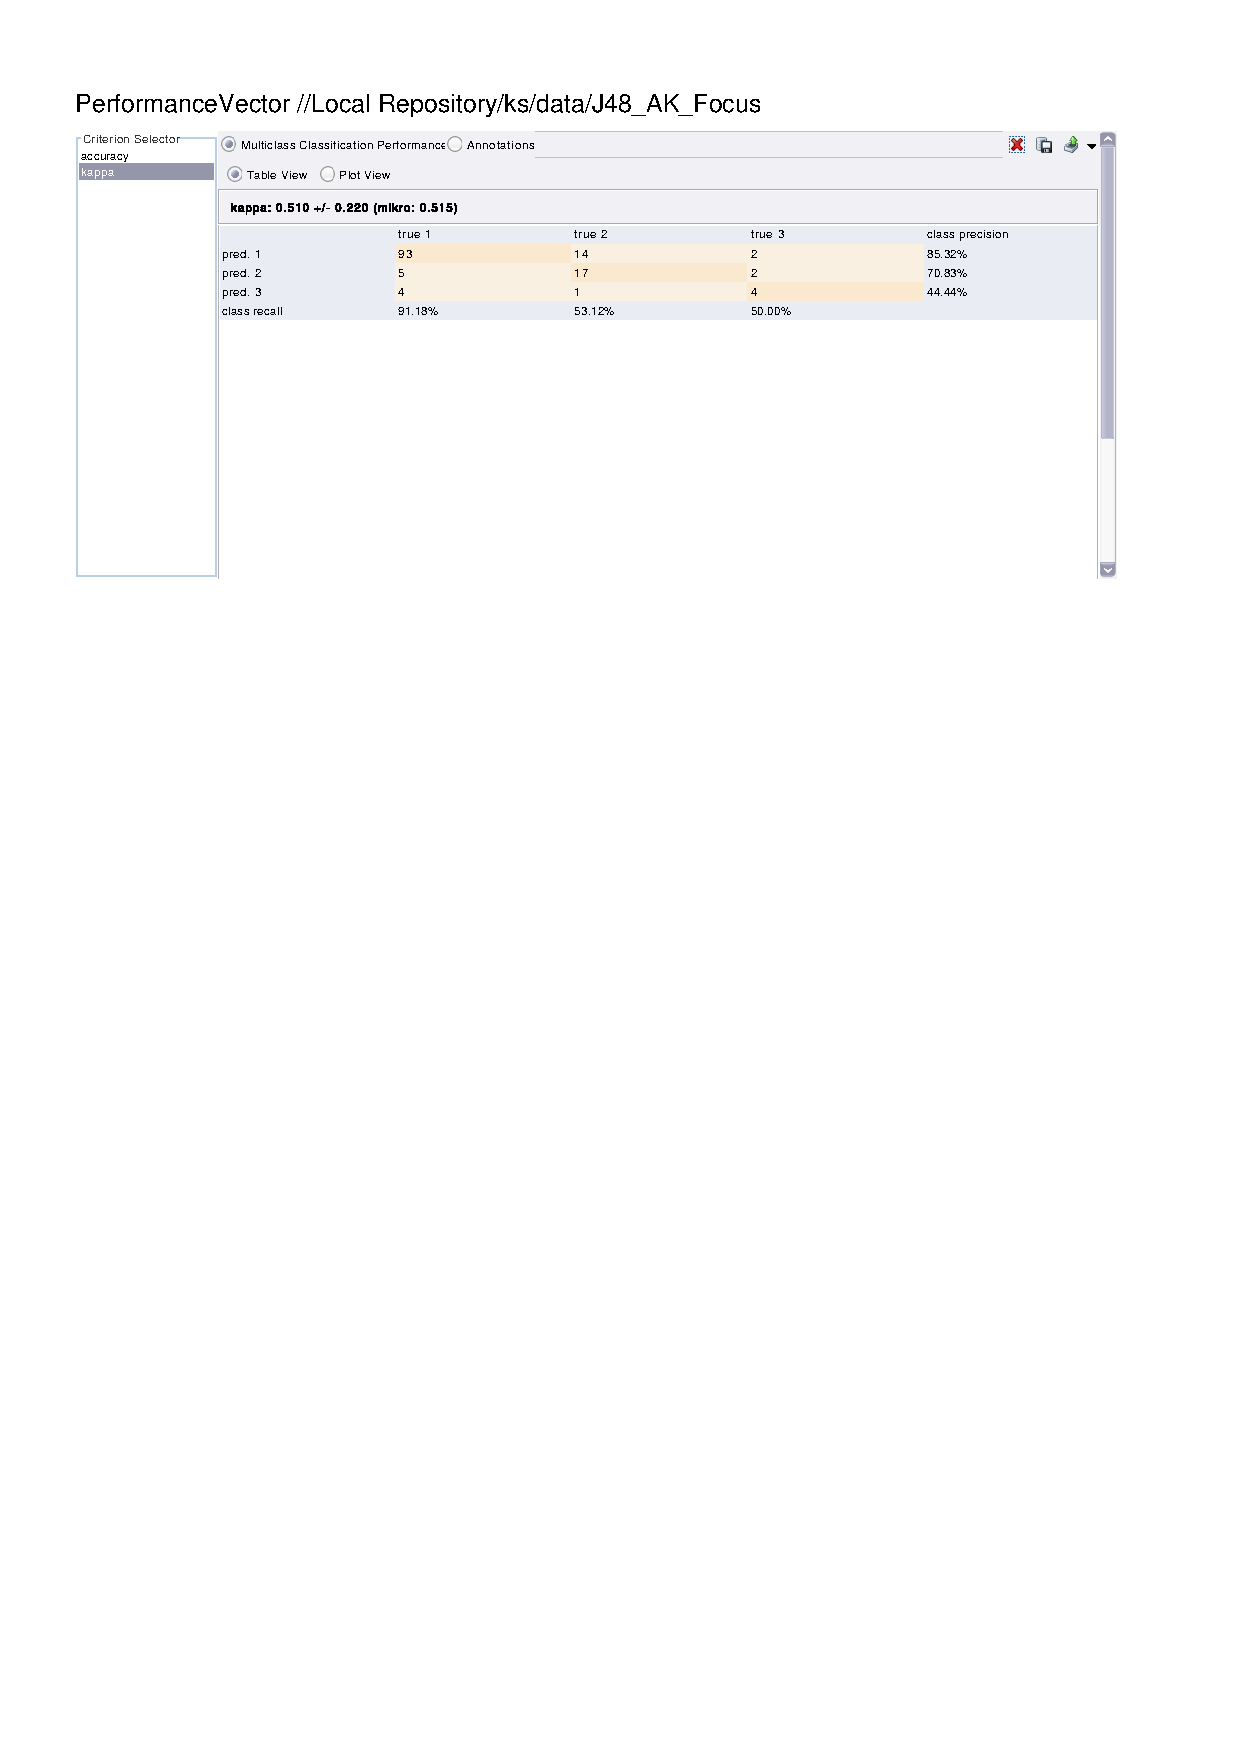
\includegraphics[trim=0 683 0 60,clip,width=16.09cm]{results/J48_K_Focus.pdf}} \caption{
} \label{J48_K_Focus}
\end{figure}

\clearpage
\FloatBarrier
% J48 Frustration
\subsubsection{Frustración}

\begin{figure}[htp]
  \centerline{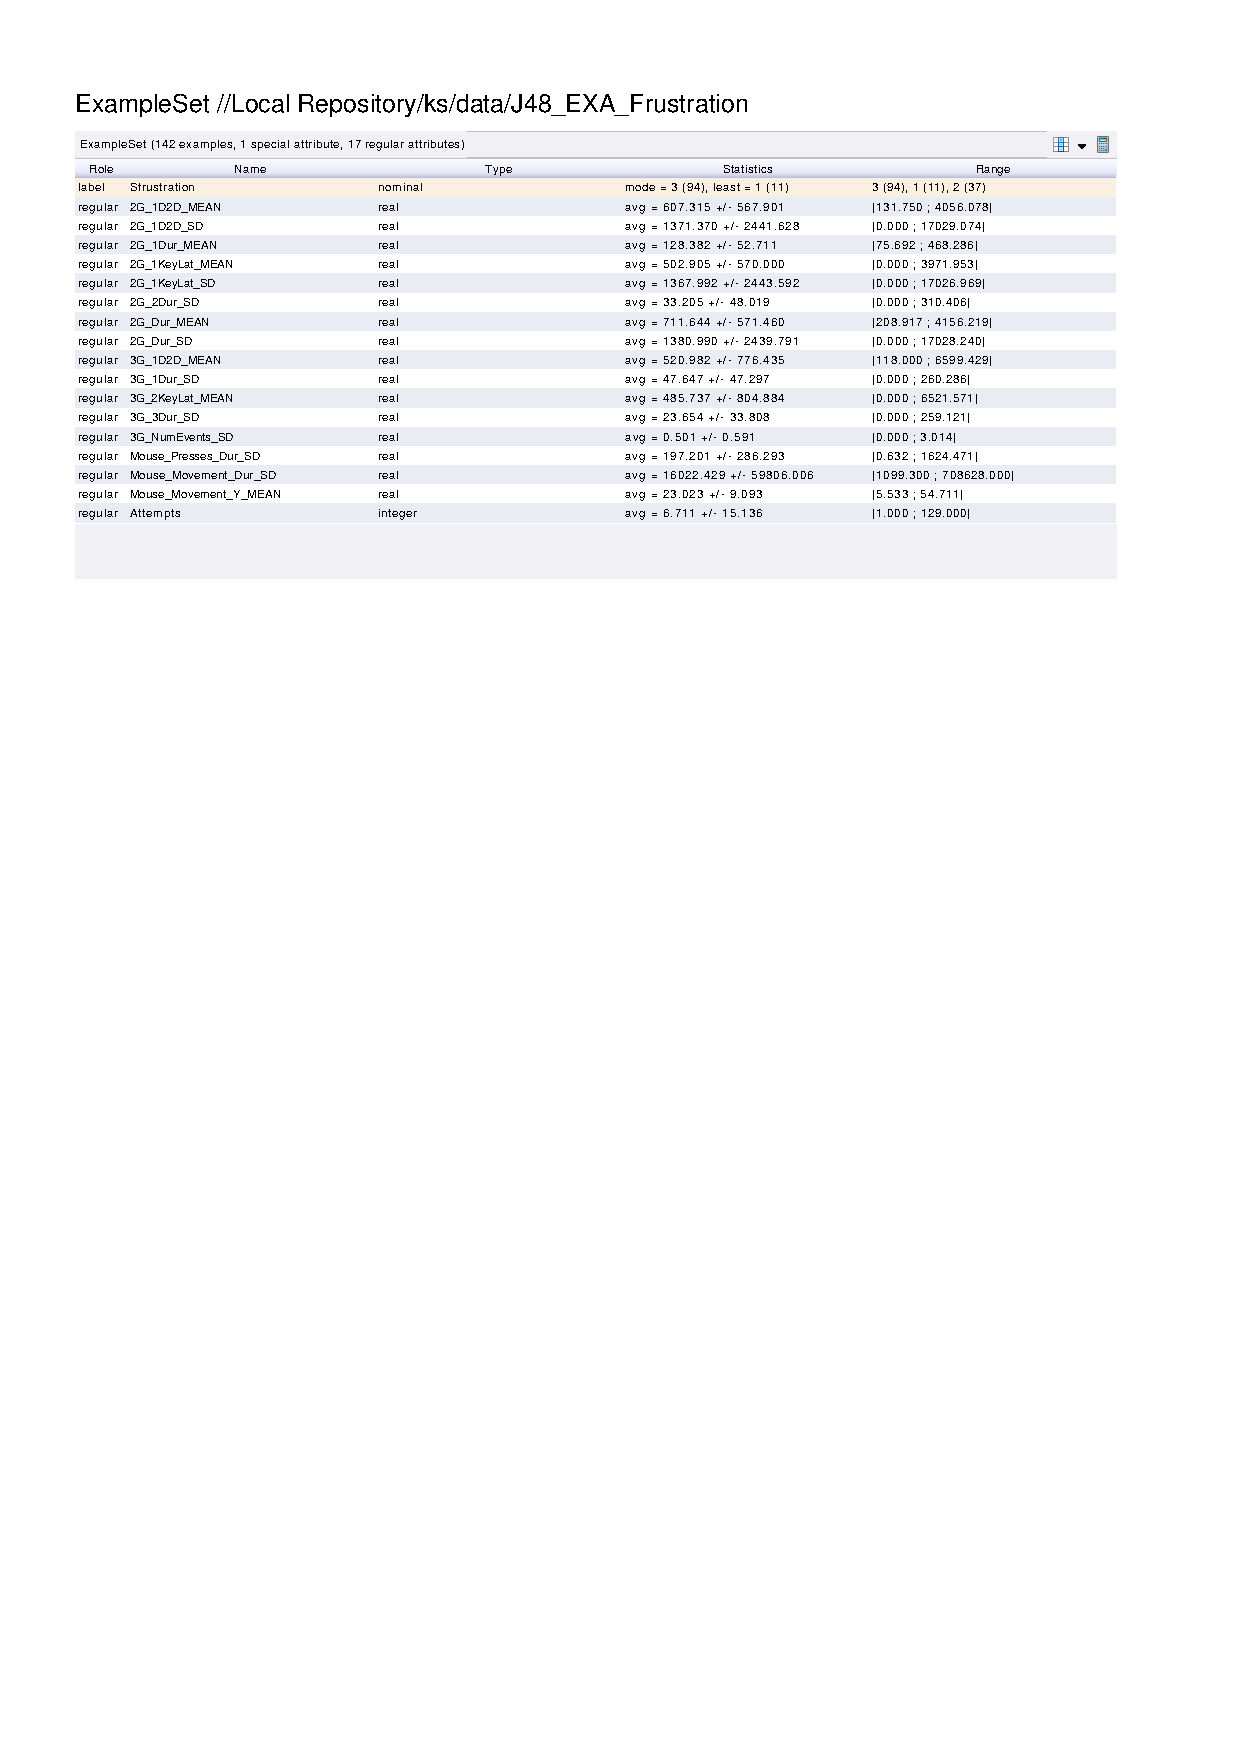
\includegraphics[trim=0 580 0 60,clip,width=16.09cm]{results/J48_EXA_Frustration.pdf}} \caption{
} \label{J48_K_Frustration}
\end{figure}

\begin{figure}[htp]
  \centerline{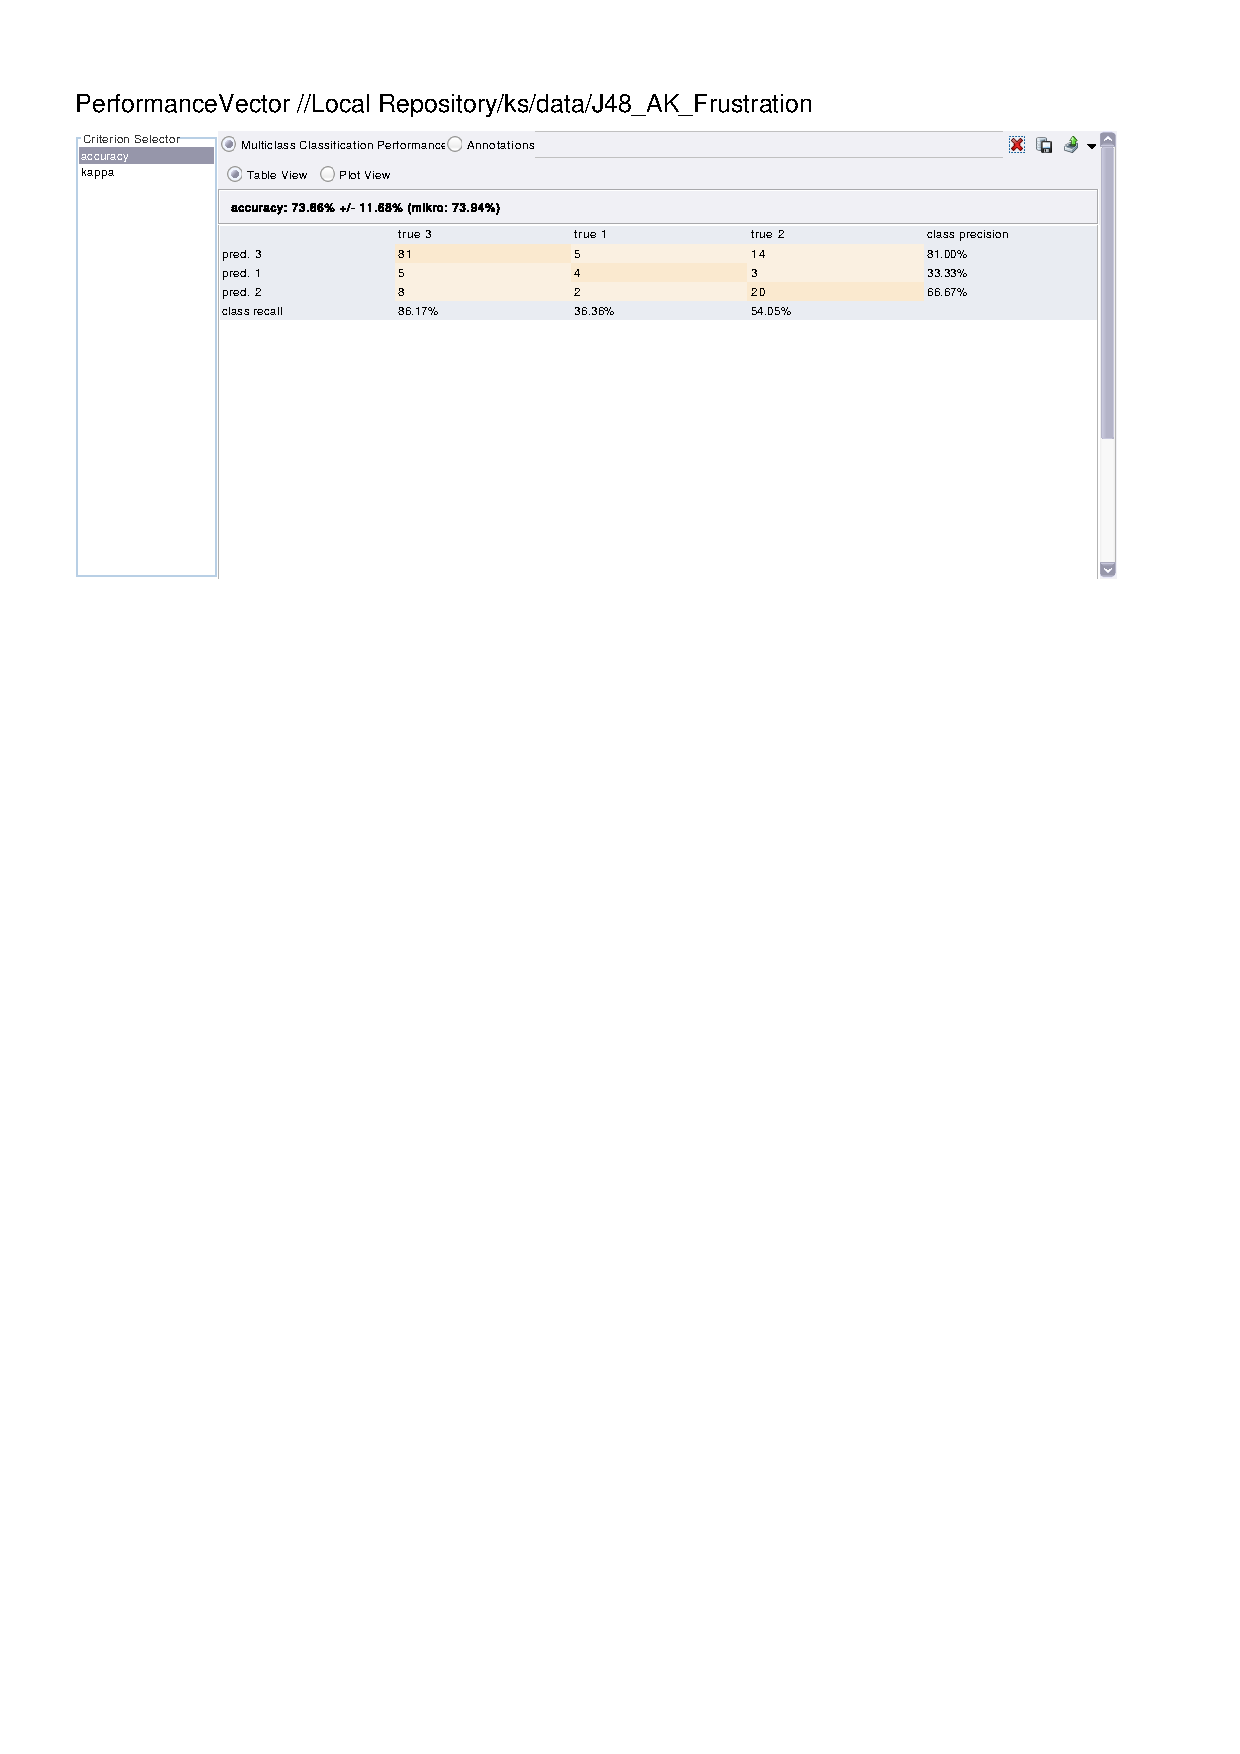
\includegraphics[trim=0 680 0 60,clip,width=16.09cm]{results/J48_A_Frustration.pdf}} \caption{
} \label{J48_K_Frustration}
\end{figure}

\begin{figure}[htp]
  \centerline{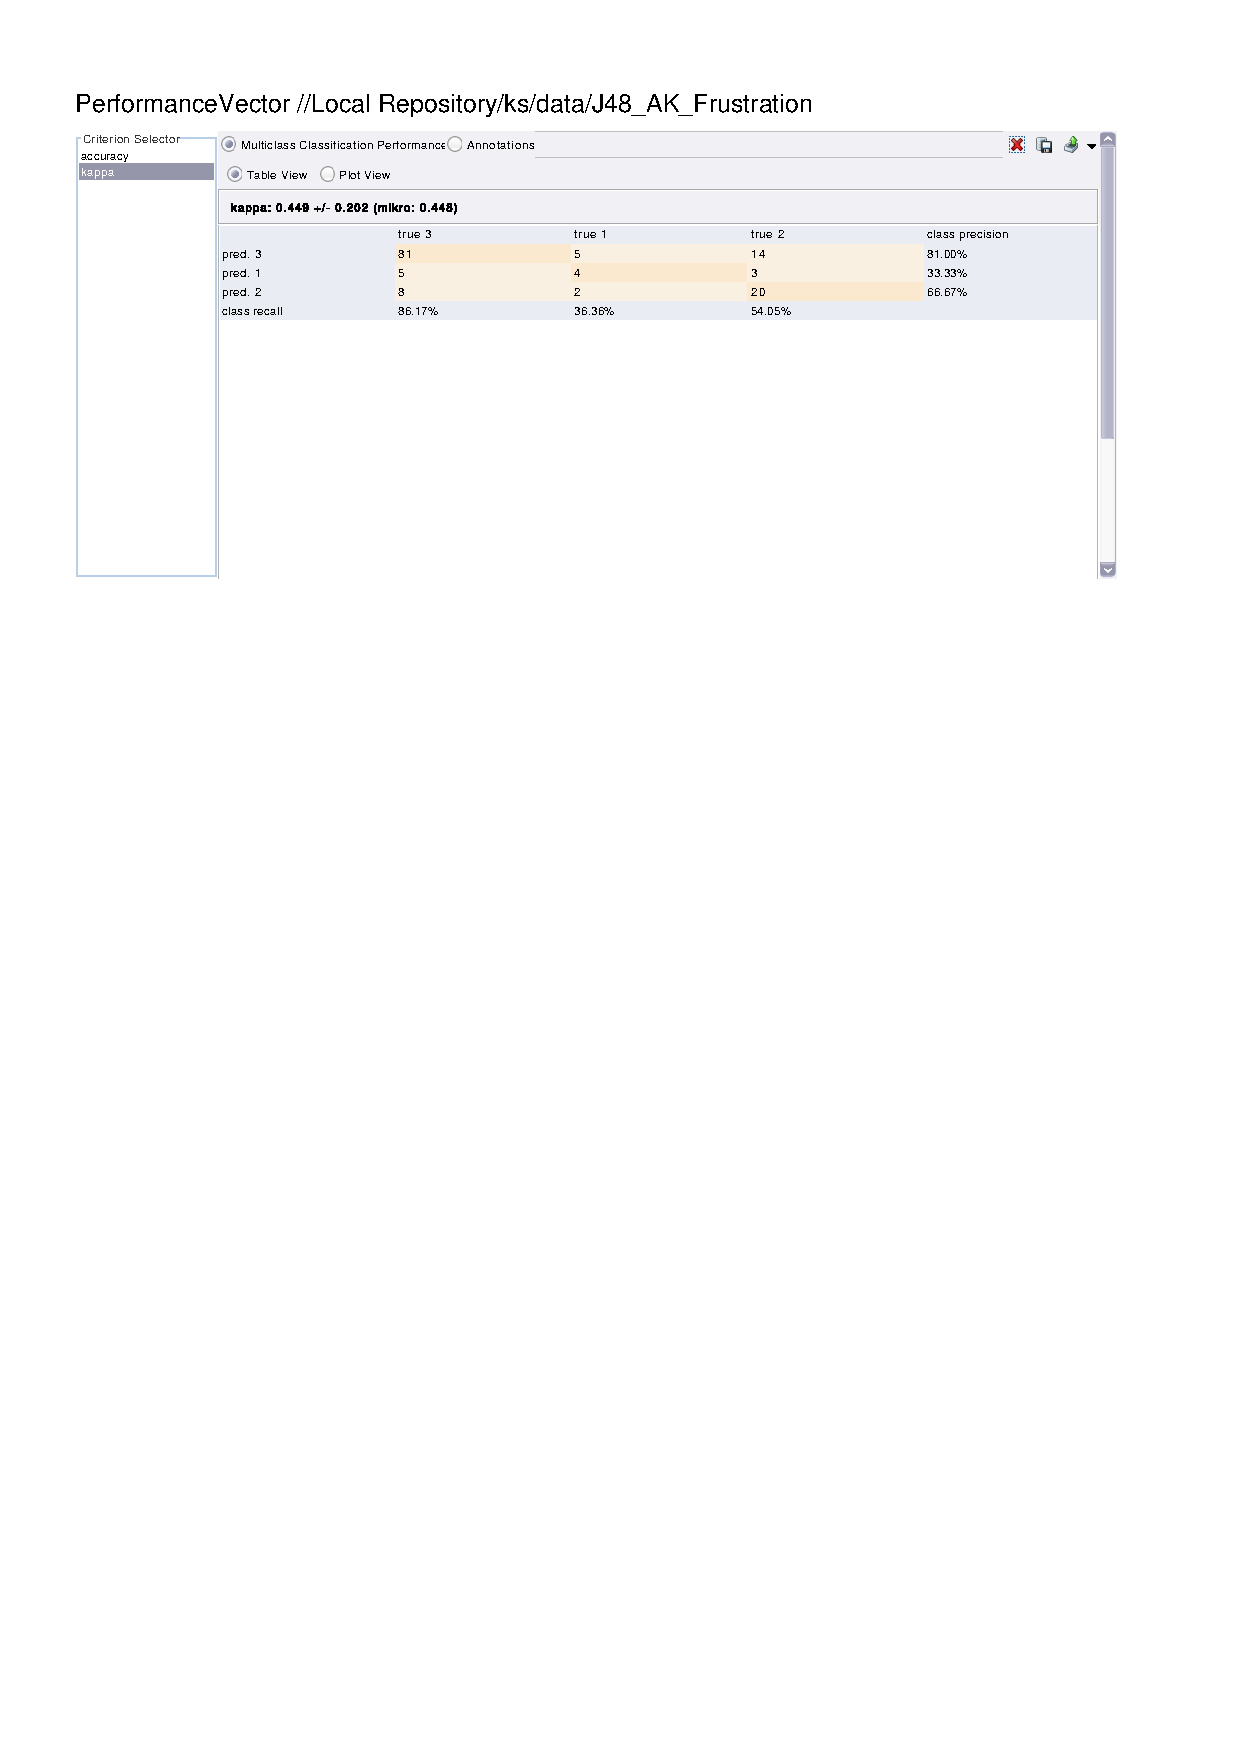
\includegraphics[trim=0 680 0 60,clip,width=16.09cm]{results/J48_K_Frustration.pdf}} \caption{
} \label{J48_K_Frustration}
\end{figure}

\clearpage
\FloatBarrier
% J48 Relaxation
\subsubsection{Relajamiento}

\begin{figure}[htp]
  \centerline{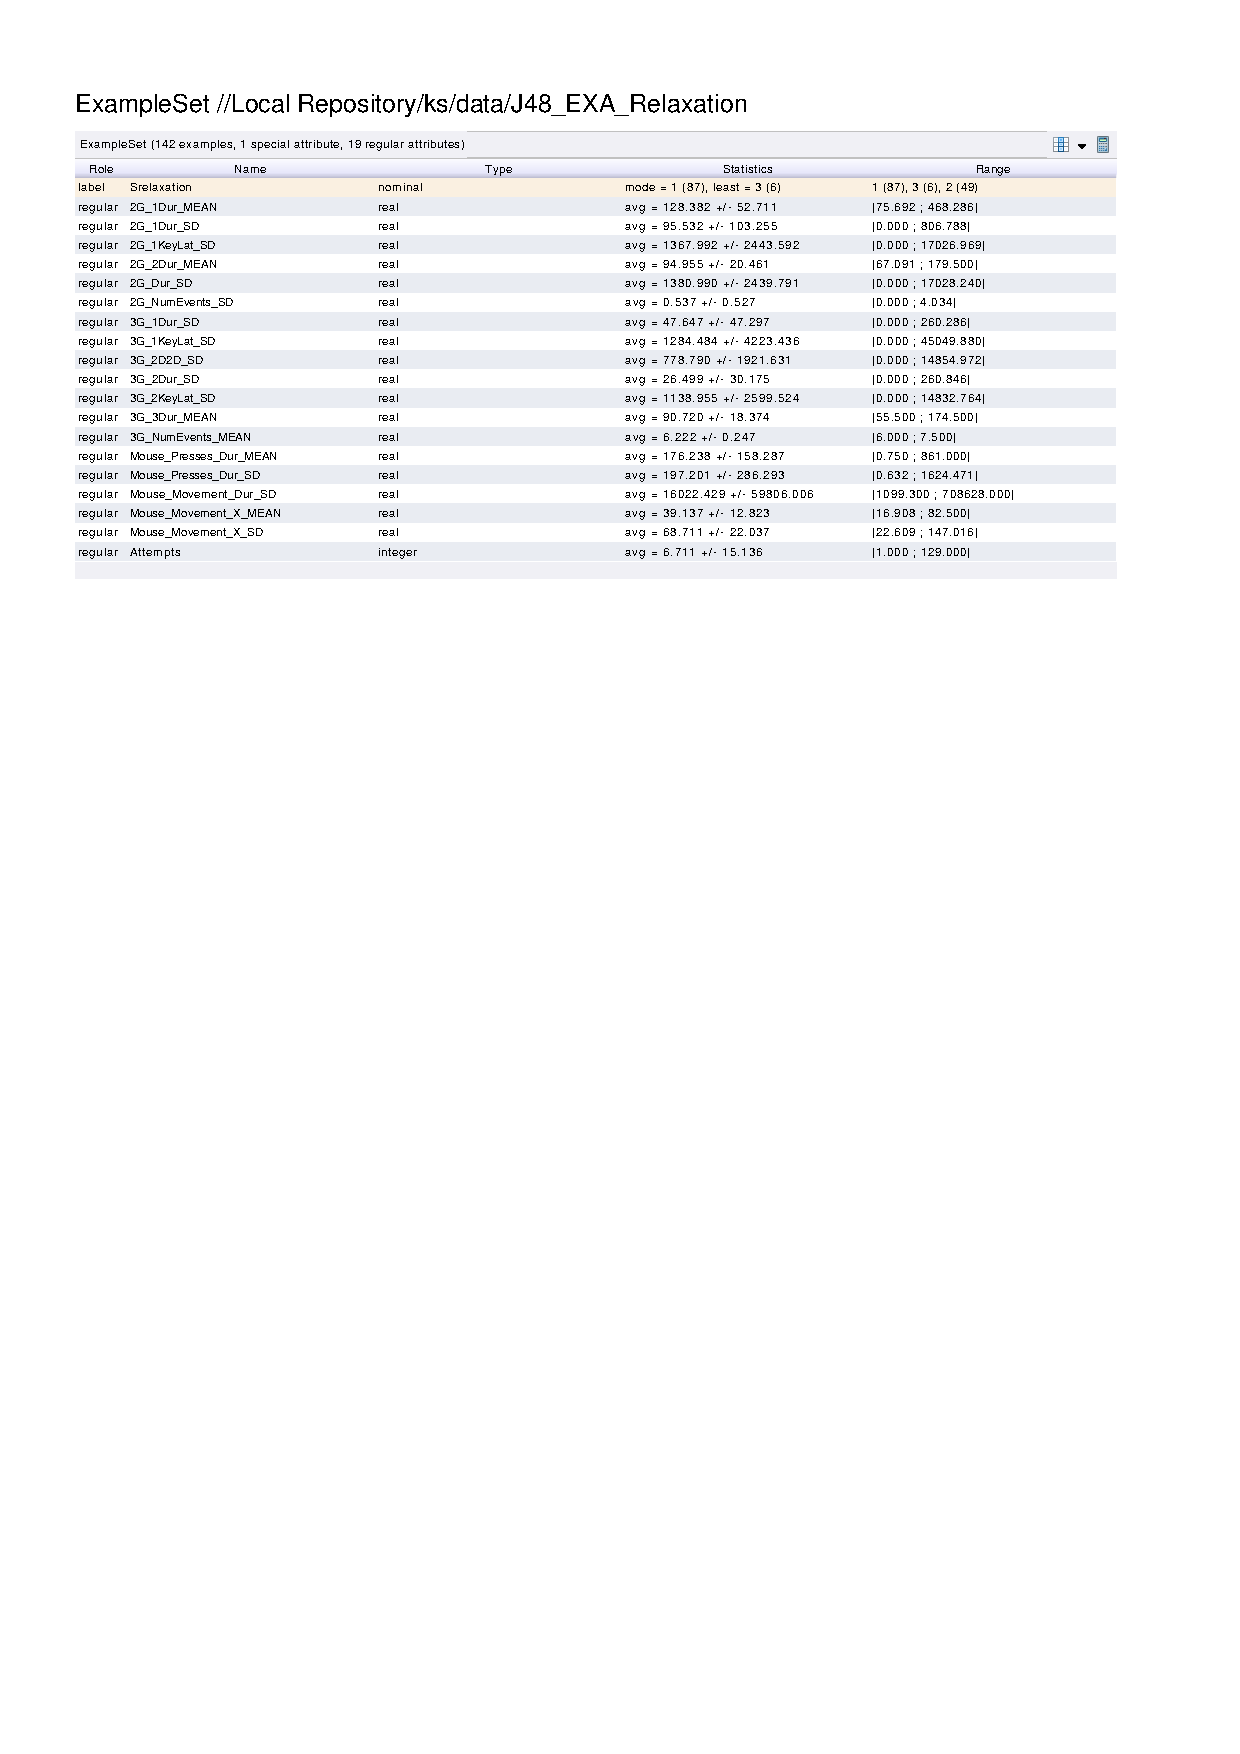
\includegraphics[trim=0 560 0 60,clip,width=16.09cm]{results/J48_EXA_Relaxation.pdf}} \caption{
} \label{J48_K_Relaxation}
\end{figure}

\begin{figure}[htp]
  \centerline{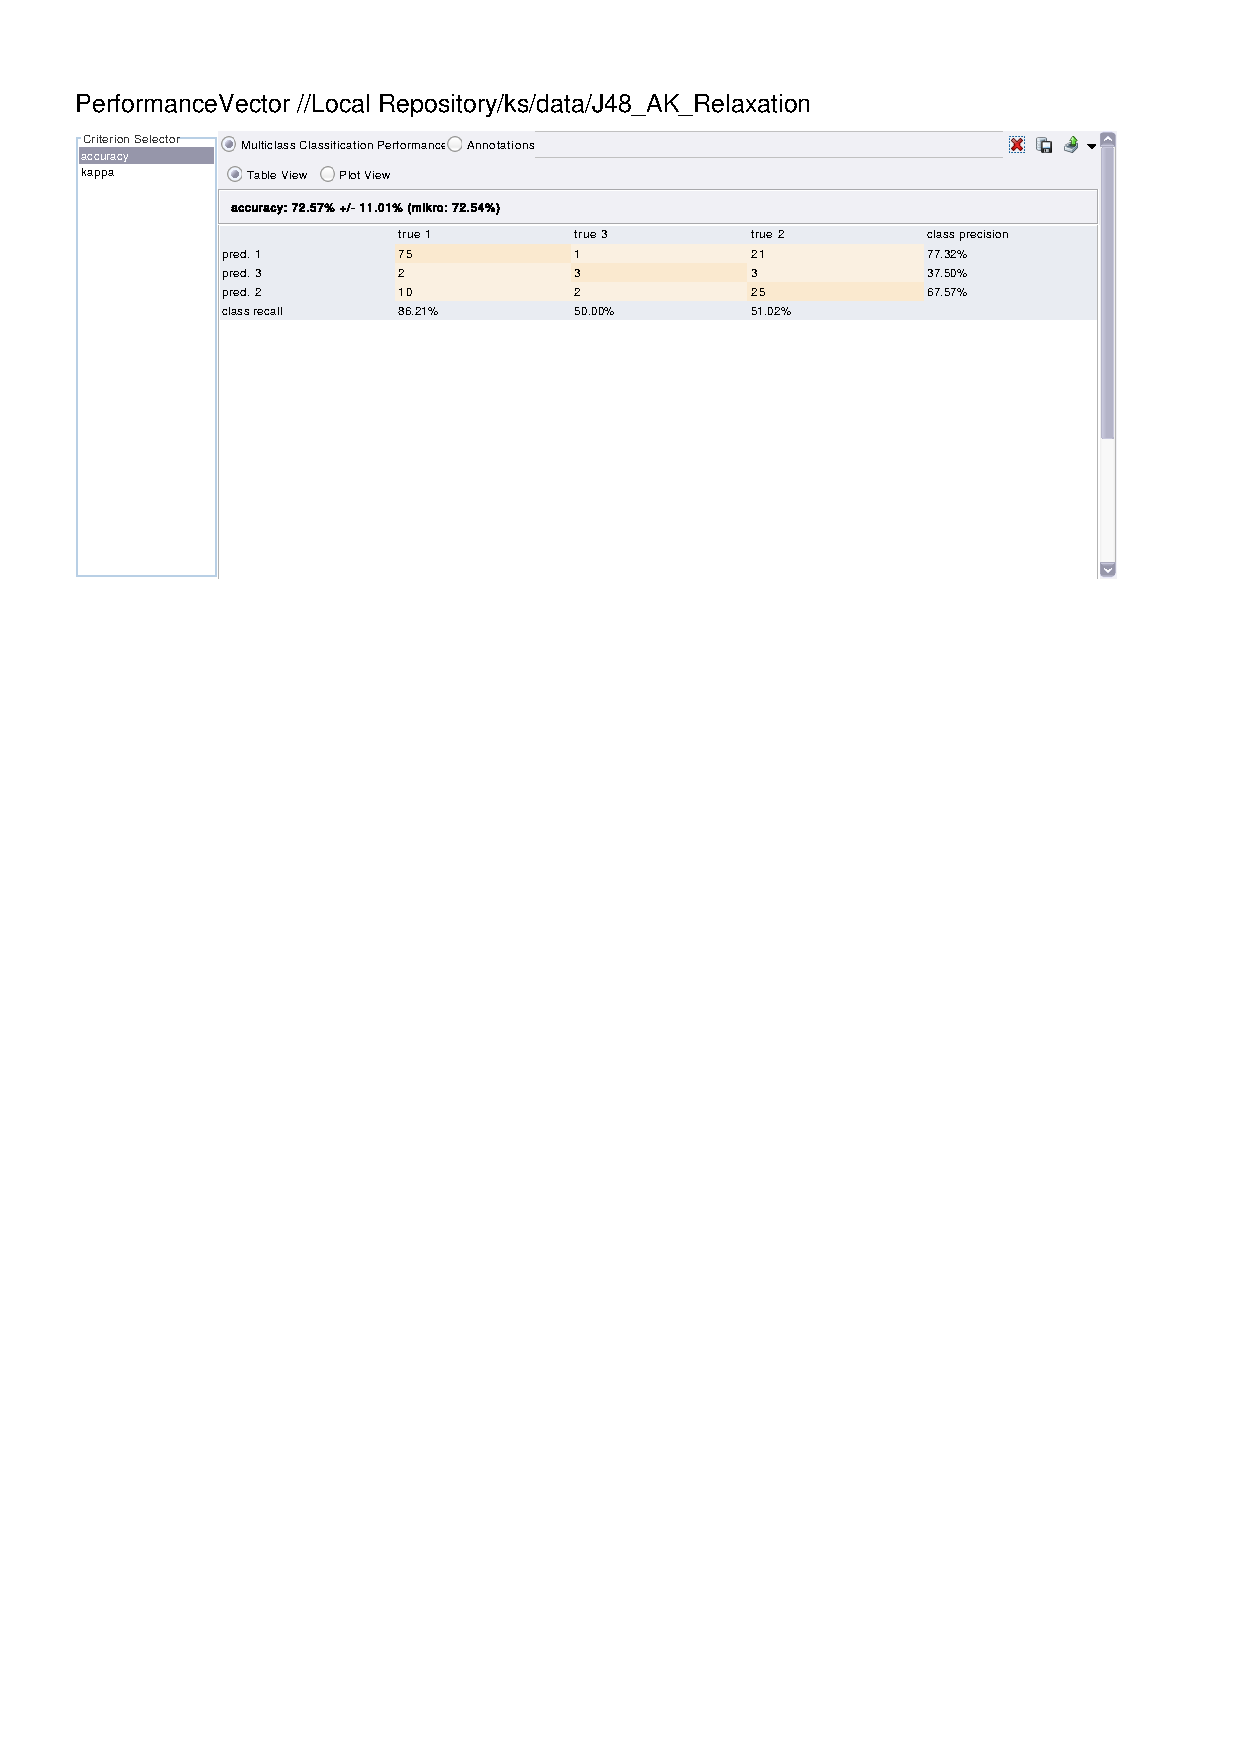
\includegraphics[trim=0 683 0 60,clip,width=16.09cm]{results/J48_A_Relaxation.pdf}} \caption{
} \label{J48_K_Relaxation}
\end{figure}

\begin{figure}[htp]
  \centerline{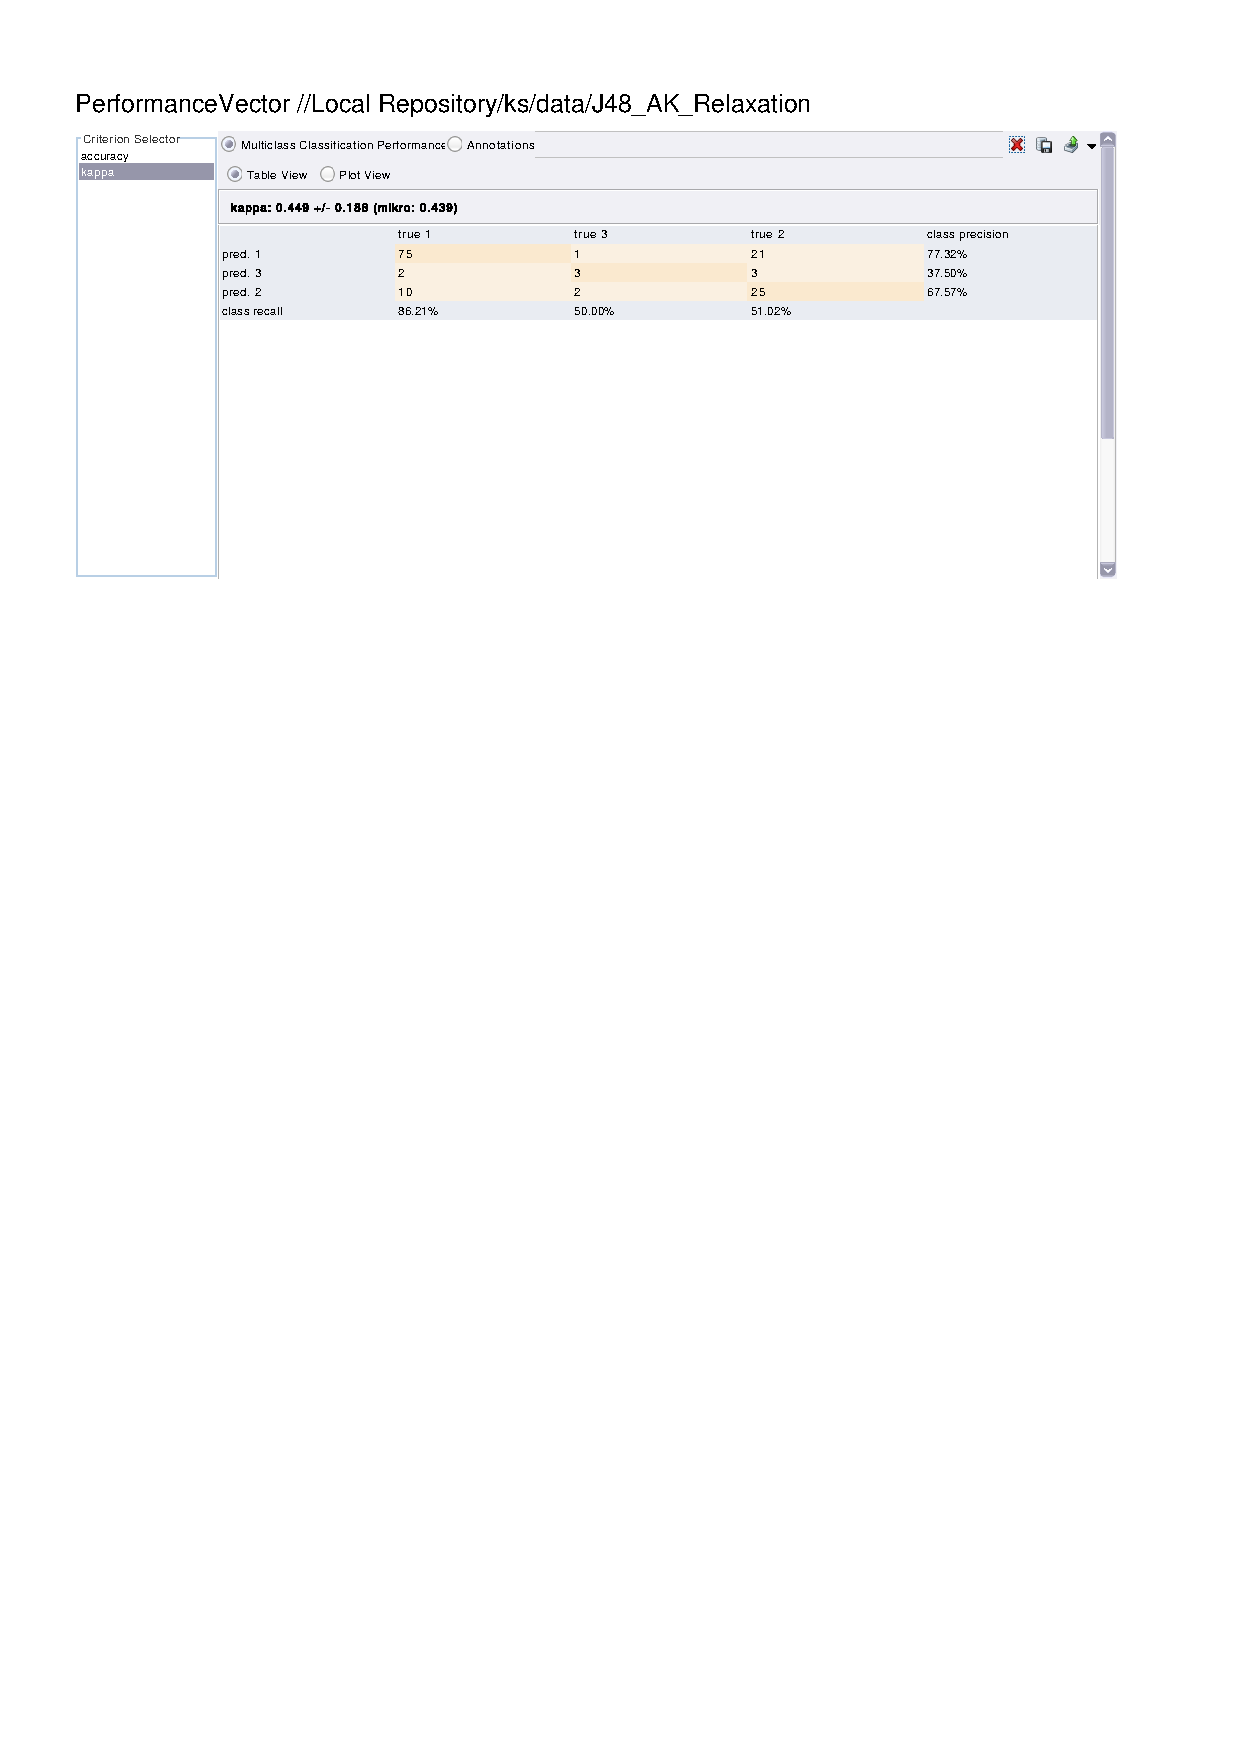
\includegraphics[trim=0 683 0 60,clip,width=16.09cm]{results/J48_K_Relaxation.pdf}} \caption{
} \label{J48_K_Relaxation}
\end{figure}

\clearpage
\FloatBarrier
\subsection{k Vecinos más Cercanos}
\subsection{Aburrimiento}

% kNN Boredom

\begin{figure}[htp]
  \centerline{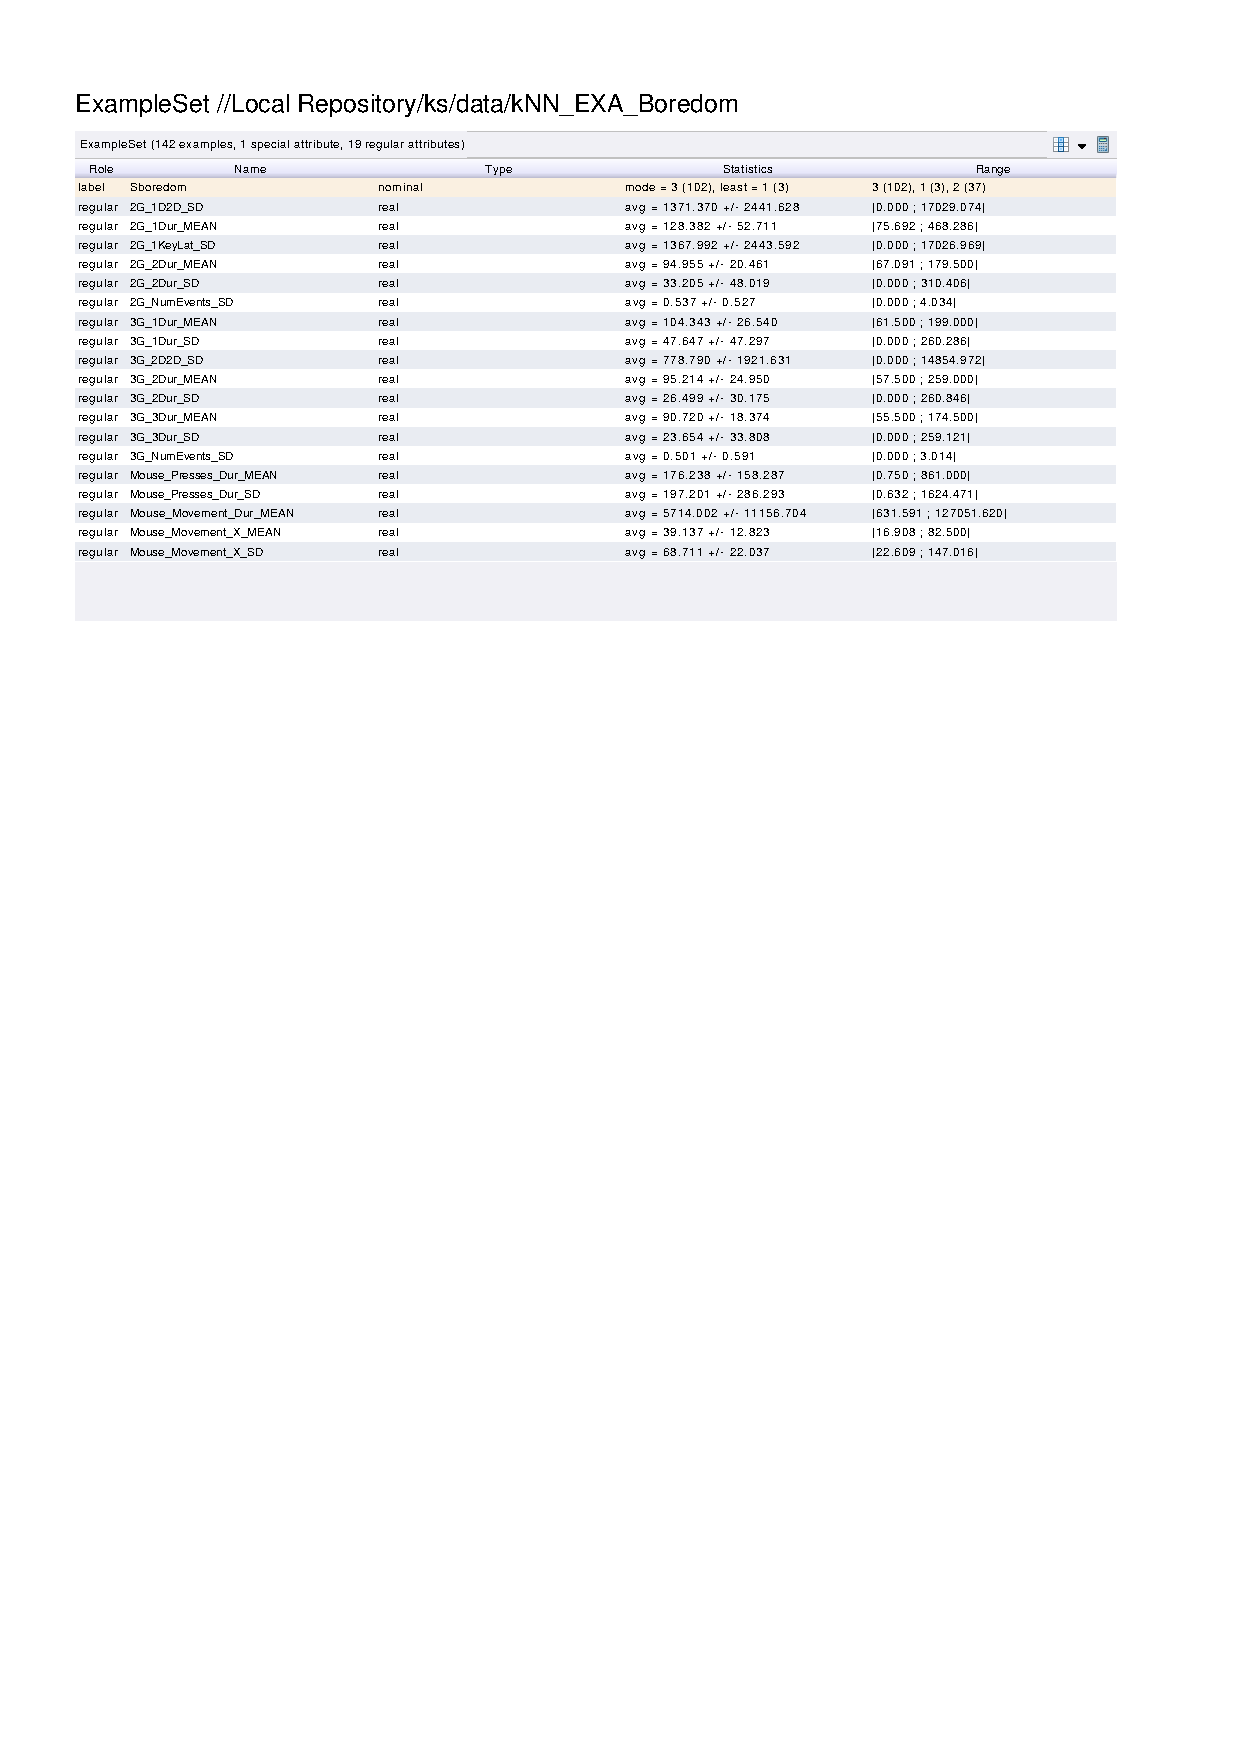
\includegraphics[trim=0 570 0 60,clip,width=16.09cm]{results/kNN_EXA_Boredom.pdf}} \caption{
} \label{kNN_EXA_Boredom}
\end{figure}

\begin{figure}[htp]
  \centerline{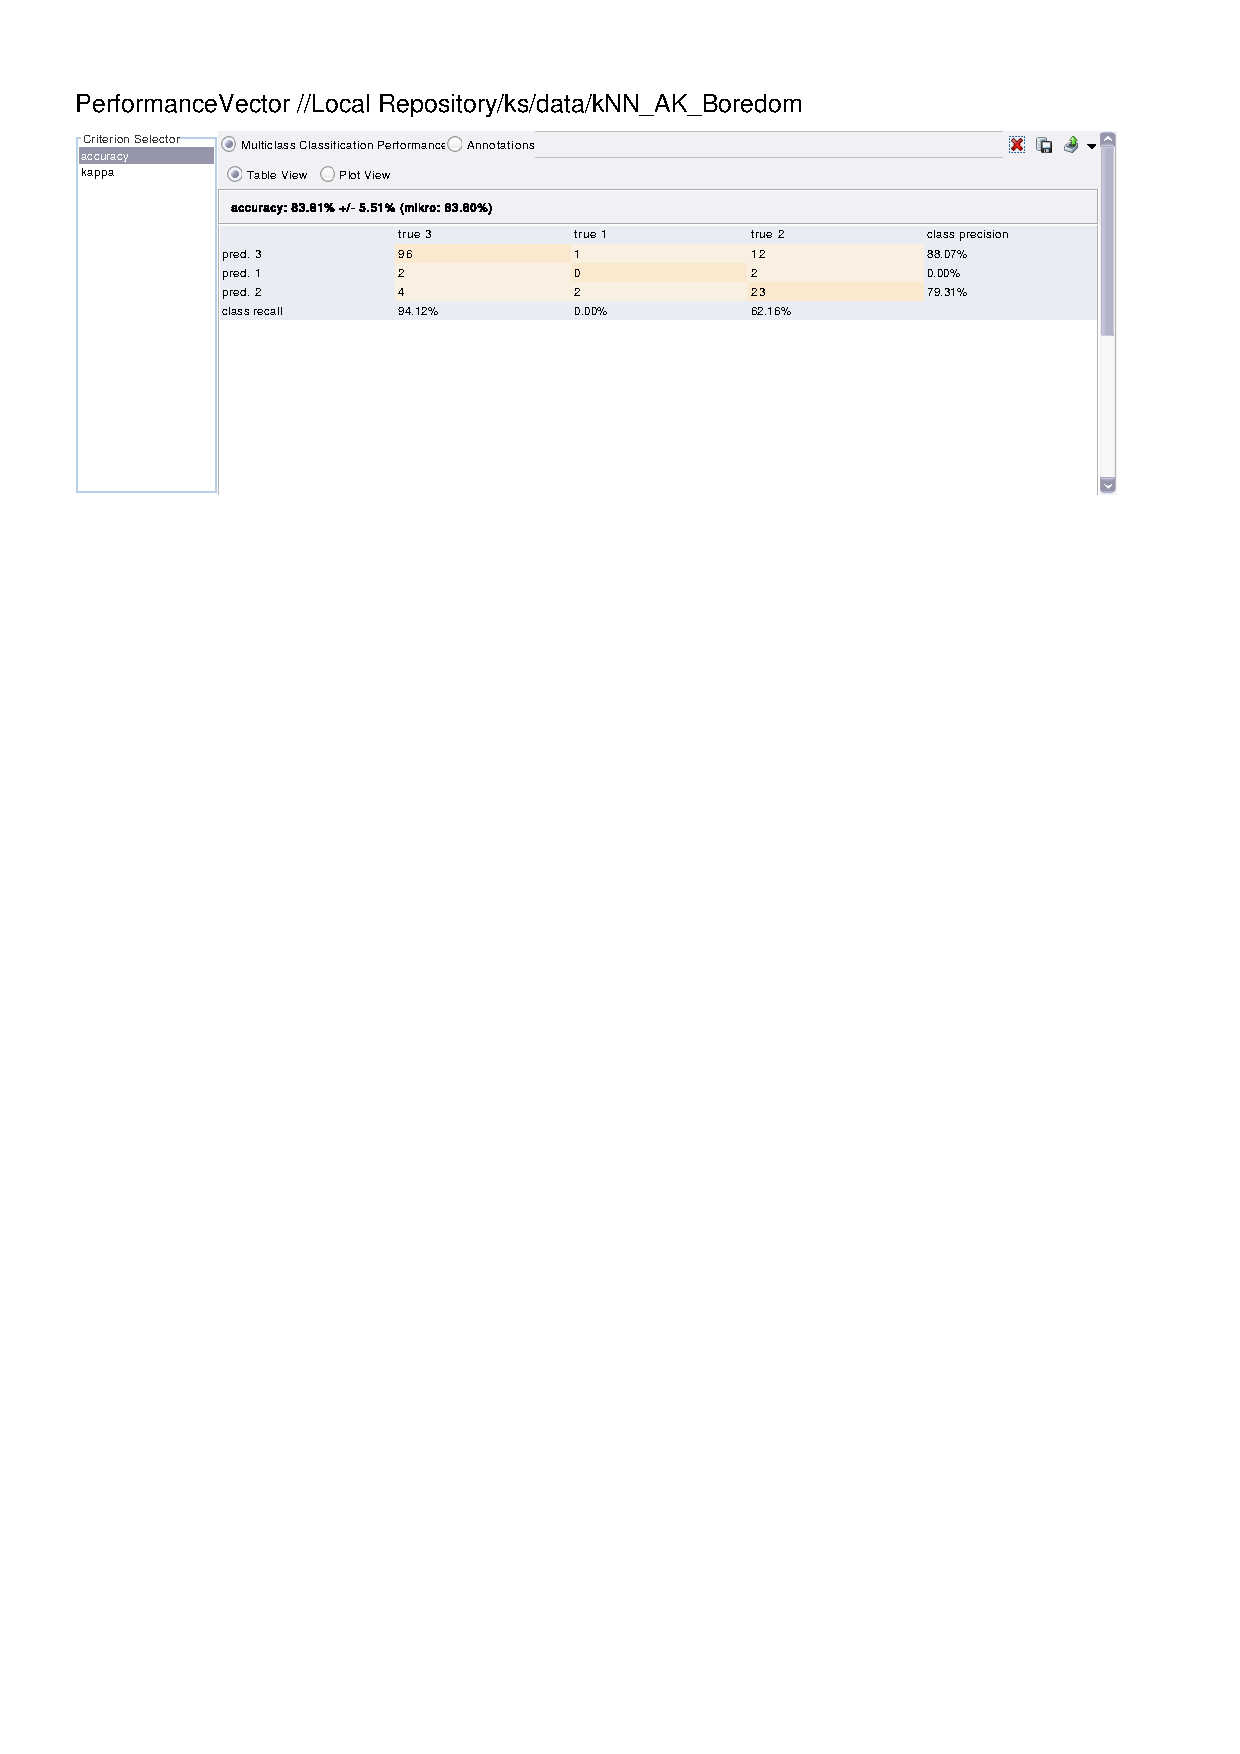
\includegraphics[trim=0 680 0 60,clip,width=16.09cm]{results/kNN_A_Boredom.pdf}} \caption{
} \label{kNN_A_Boredom}
\end{figure}

\begin{figure}[htp]
  \centerline{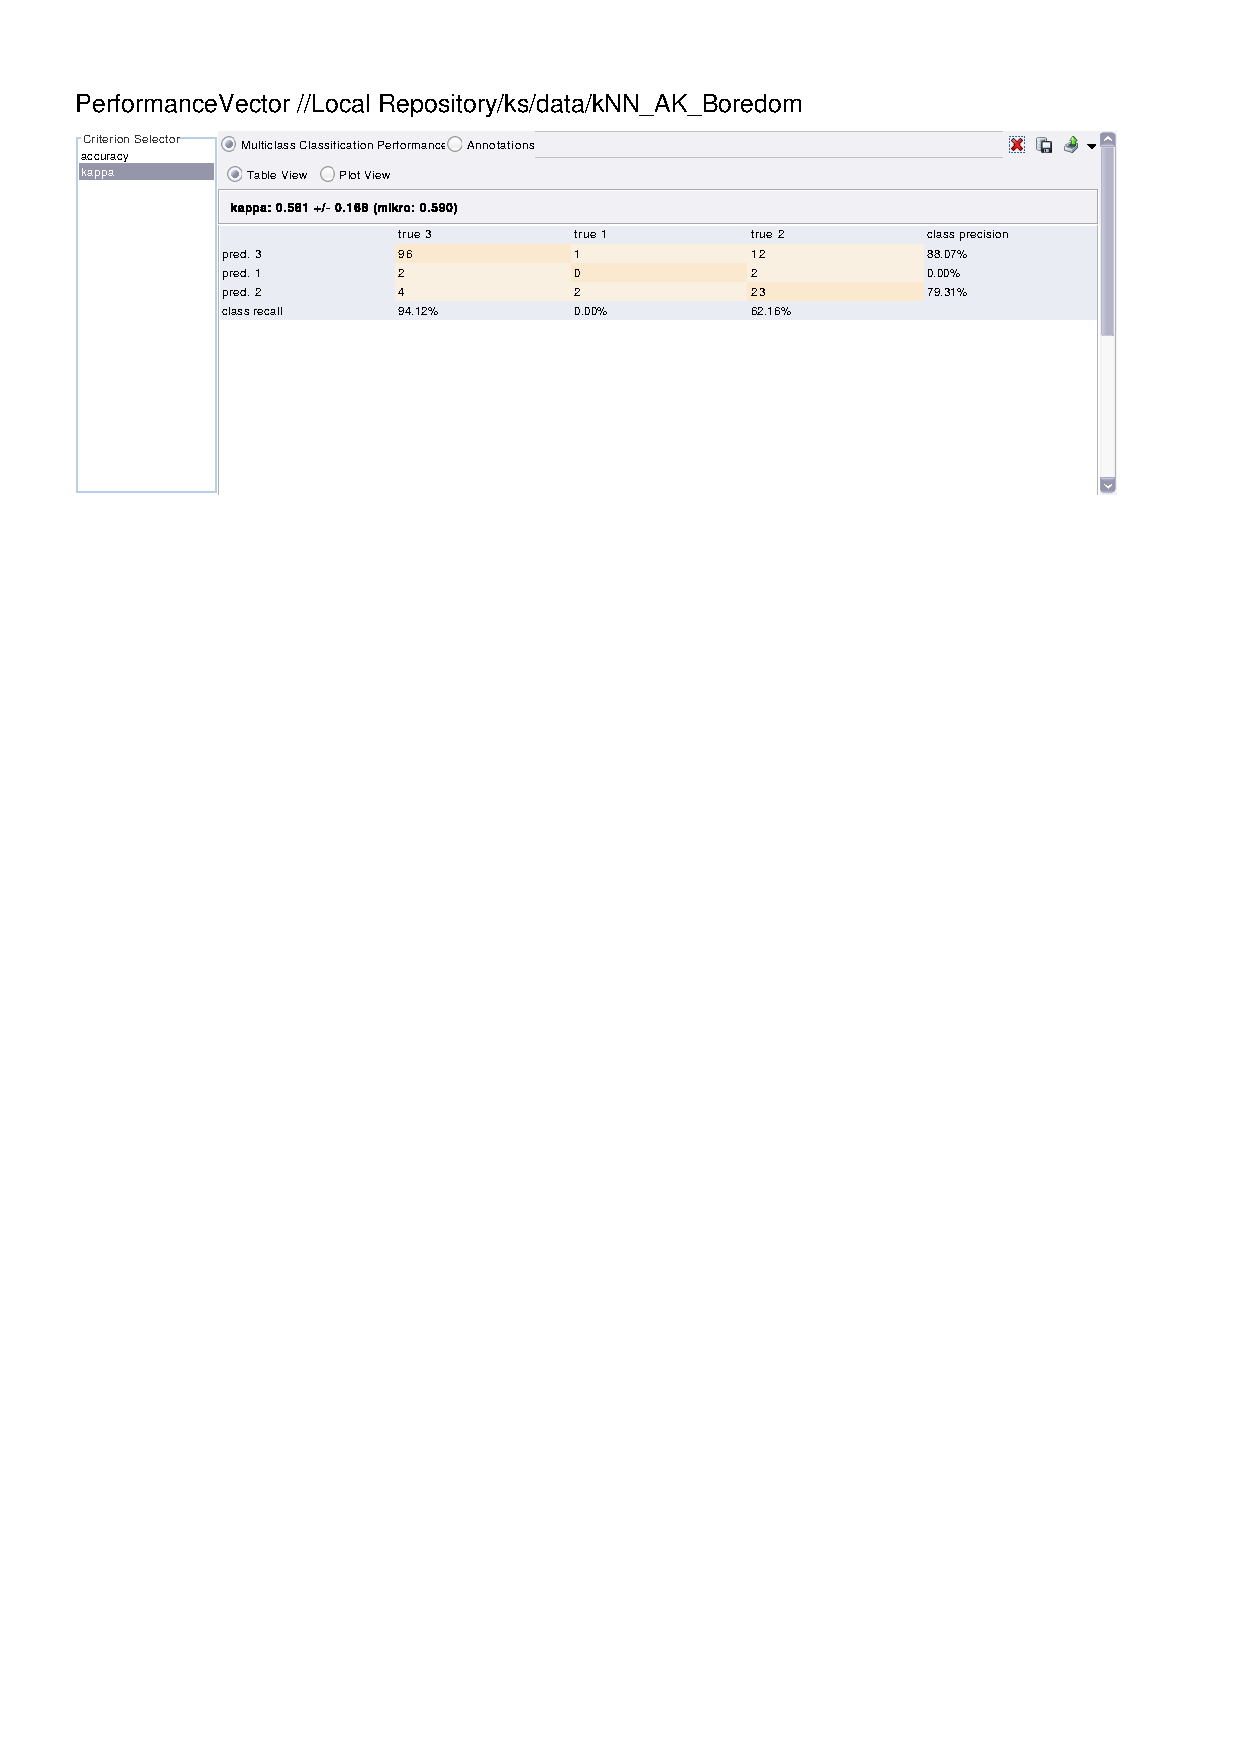
\includegraphics[trim=0 680 0 60,clip,width=16.09cm]{results/kNN_K_Boredom.pdf}} \caption{
} \label{kNN_K_Boredom}
\end{figure}

\clearpage
\FloatBarrier
\subsection{Distracción}
% kNN Distraction

\begin{figure}[htp]
  \centerline{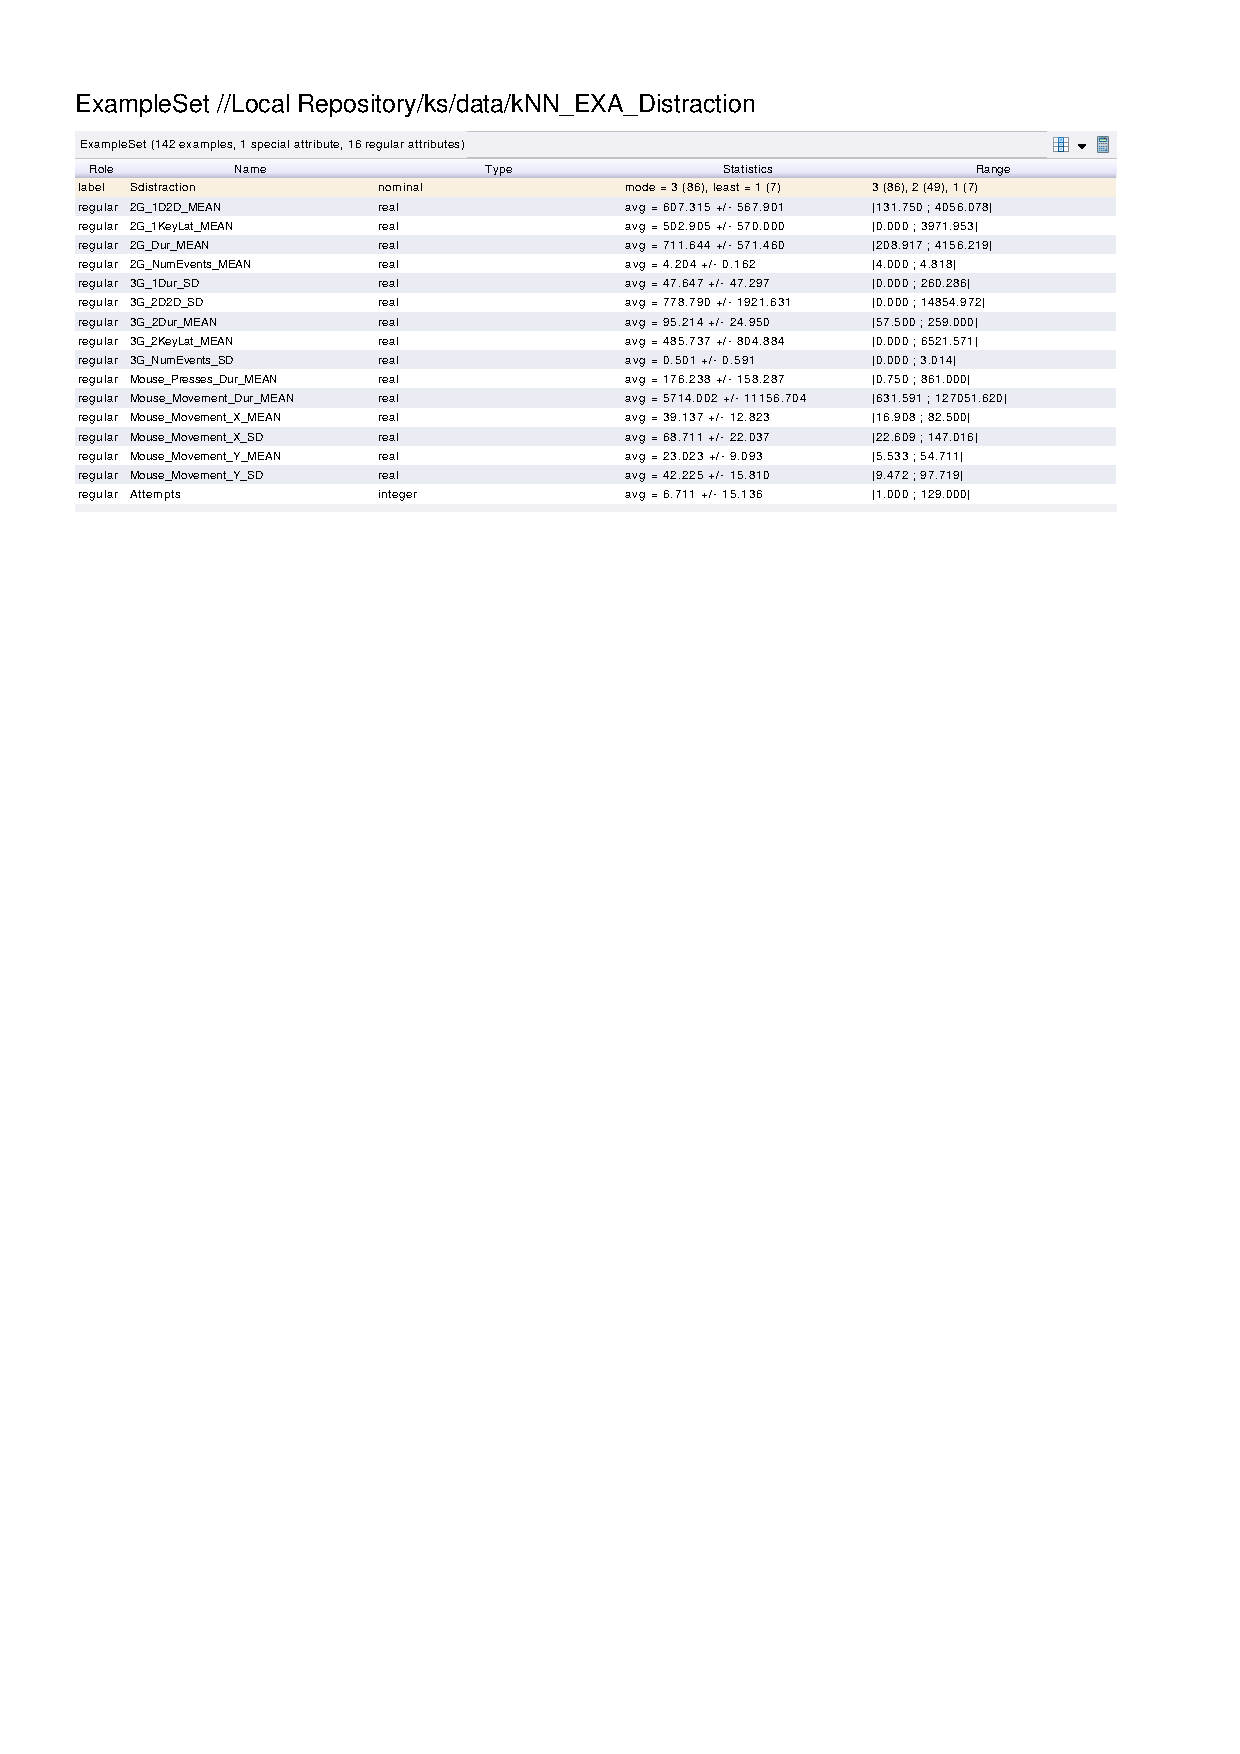
\includegraphics[trim=0 580 0 60,clip,width=16.09cm]{results/kNN_EXA_Distraction.pdf}} \caption{
} \label{kNN_EXA_Distraction}
\end{figure}

\begin{figure}[htp]
  \centerline{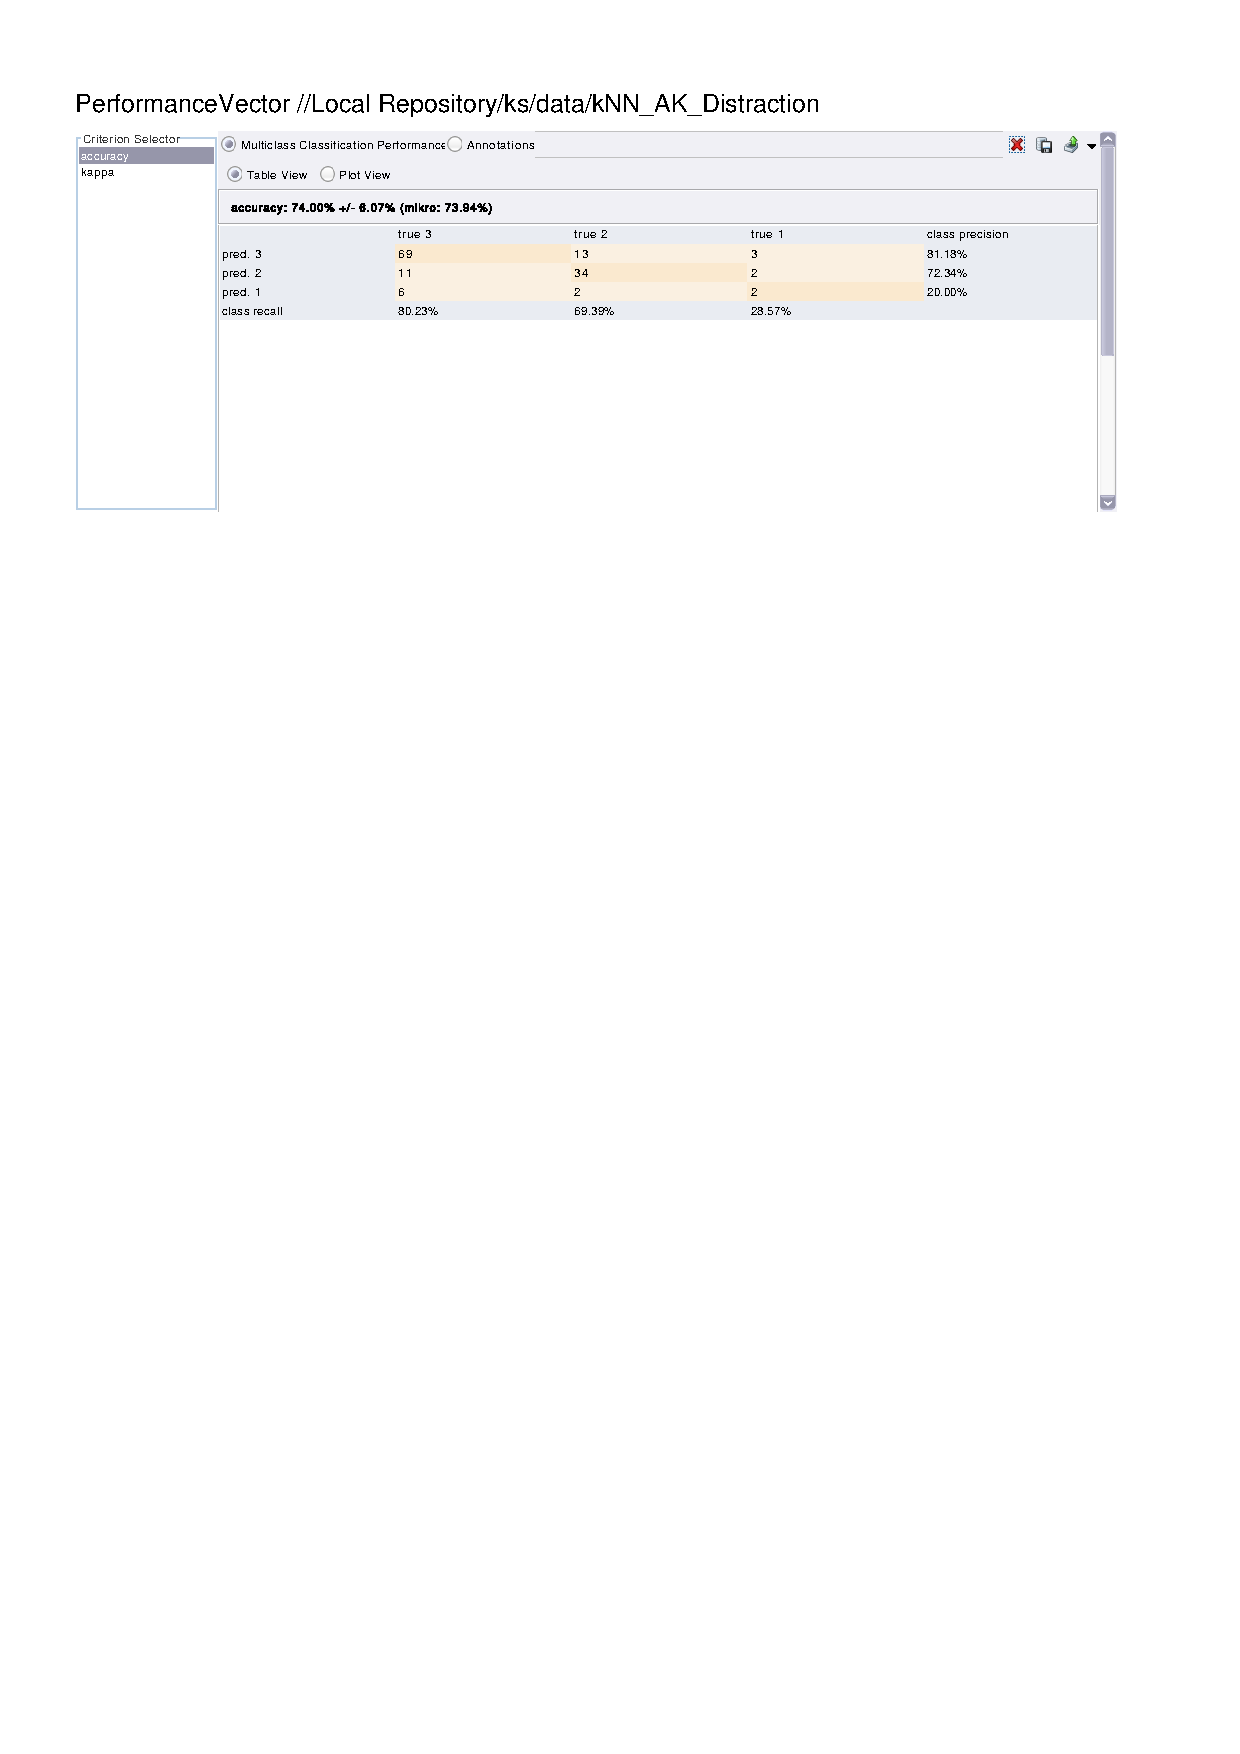
\includegraphics[trim=0 680 0 60,clip,width=16.09cm]{results/kNN_A_Distraction.pdf}} \caption{
} \label{kNN_A_Distraction}
\end{figure}

\begin{figure}[htp]
  \centerline{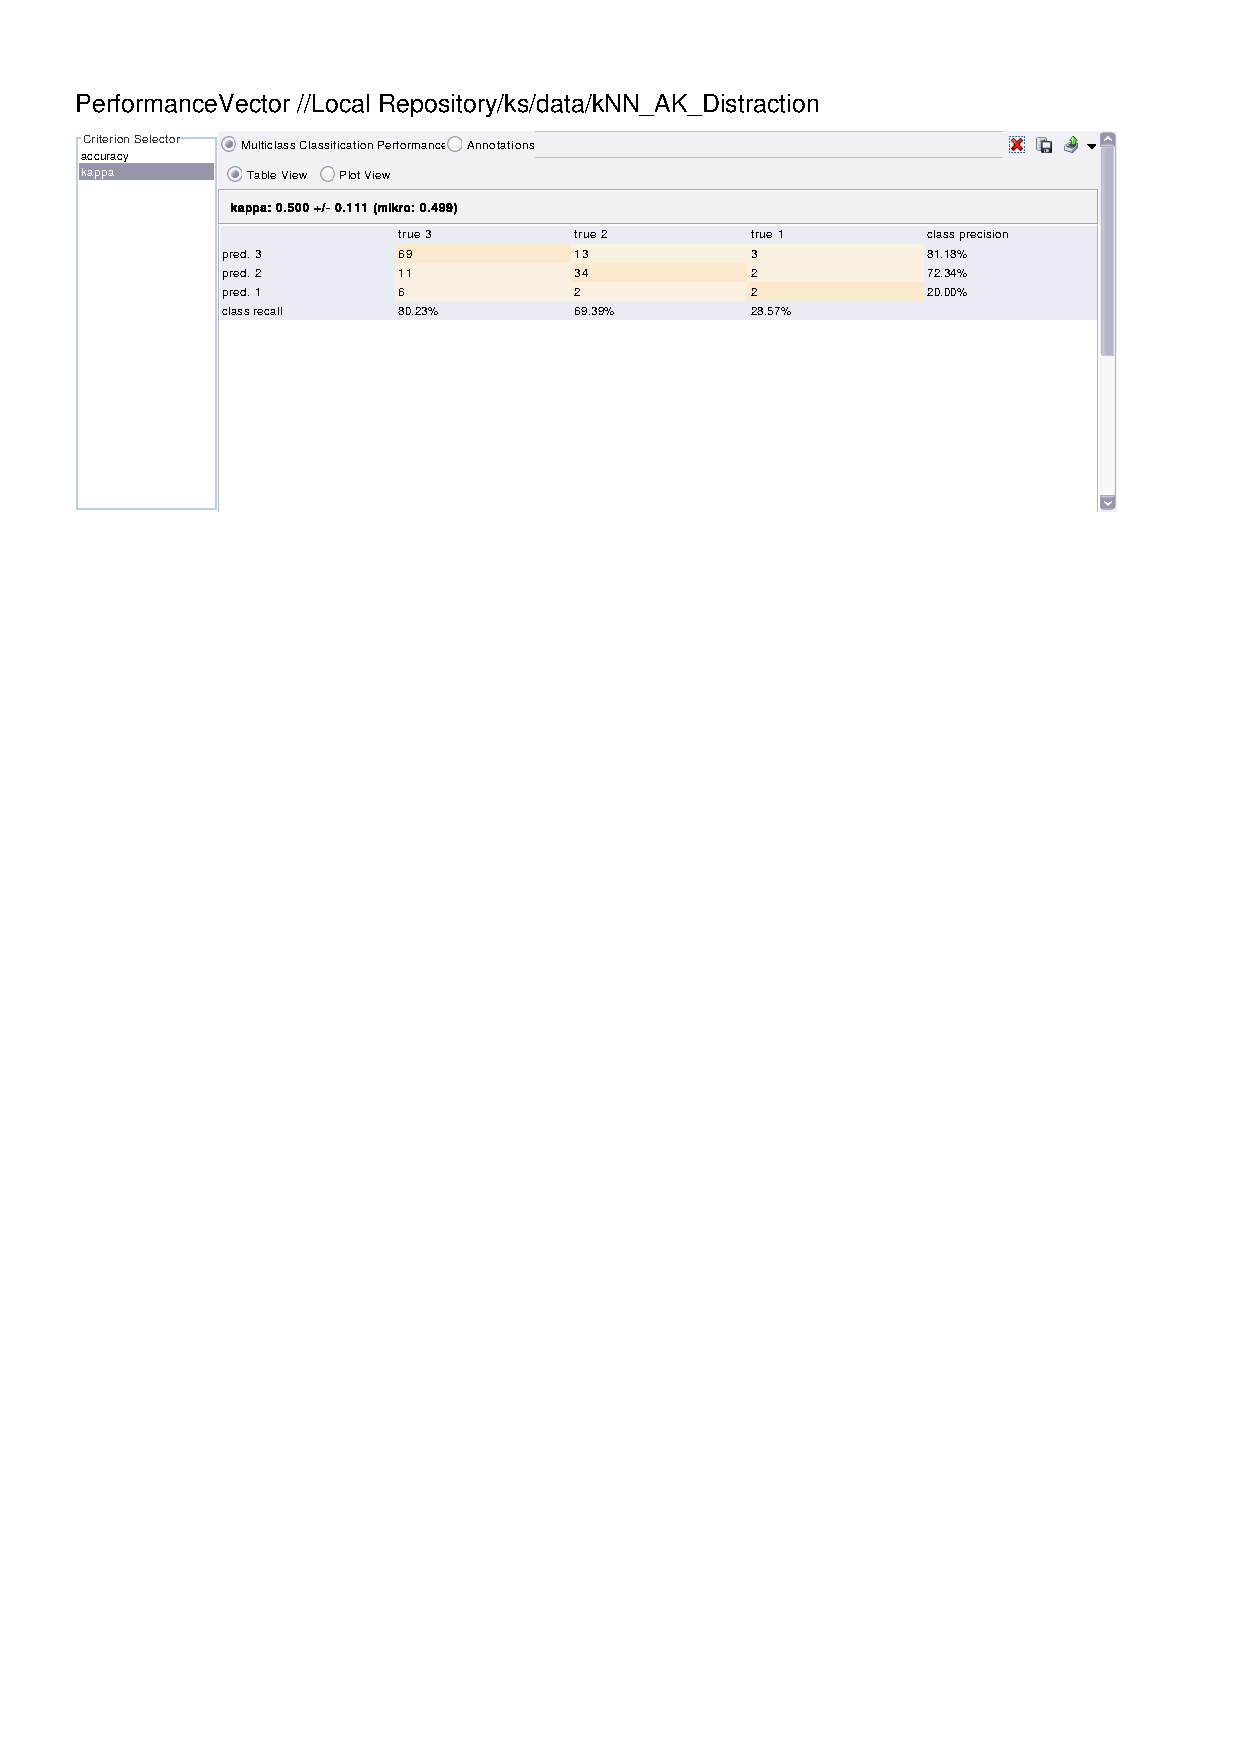
\includegraphics[trim=0 680 0 60,clip,width=16.09cm]{results/kNN_K_Distraction.pdf}} \caption{
} \label{kNN_K_Distraction}
\end{figure}

\clearpage
\FloatBarrier
\subsection{Entusiasmo}
% kNN Excitement

\begin{figure}[htp]
  \centerline{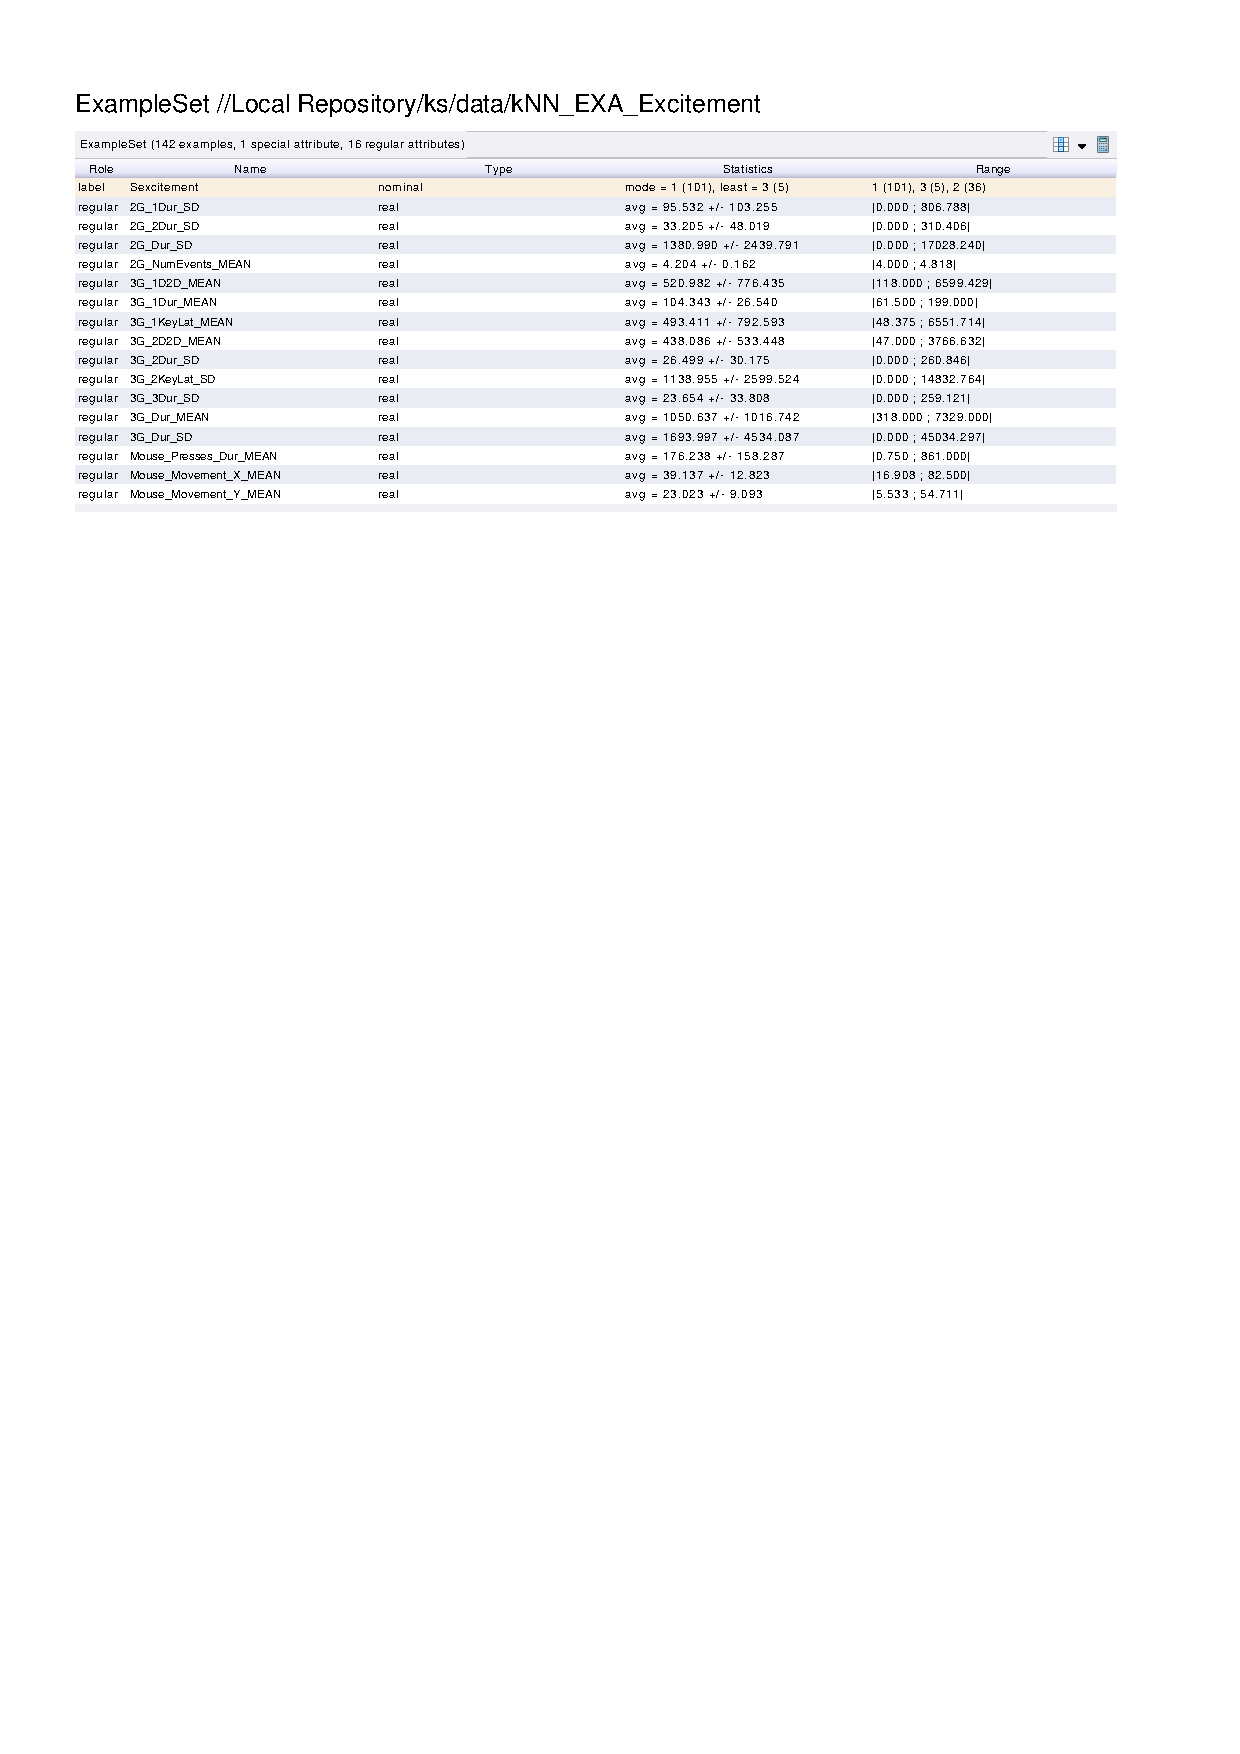
\includegraphics[trim=0 570 0 60,clip,width=16.09cm]{results/kNN_EXA_Excitement.pdf}} \caption{
} \label{kNN_K_Excitement}
\end{figure}

\begin{figure}[htp]
  \centerline{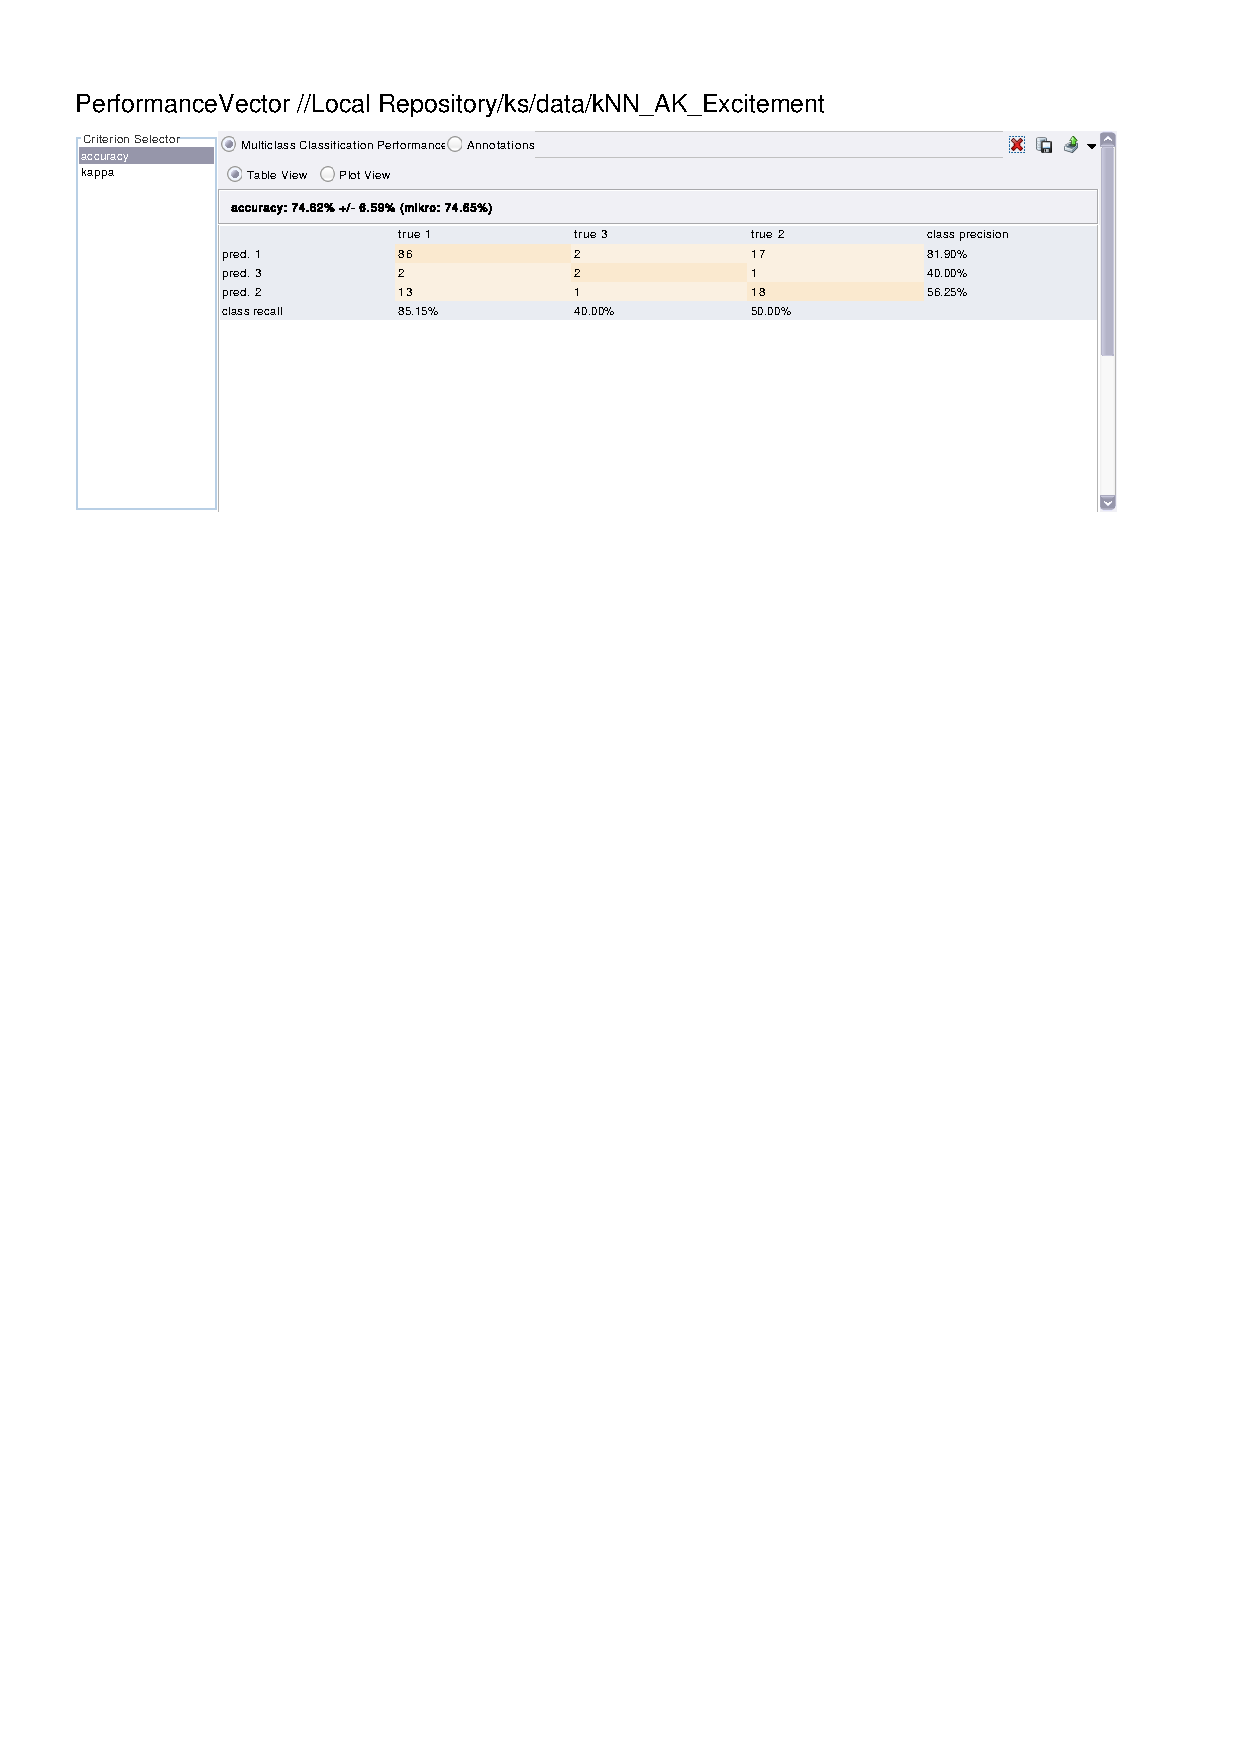
\includegraphics[trim=0 680 0 60,clip,width=16.09cm]{results/kNN_A_Excitement.pdf}} \caption{
} \label{kNN_K_Excitement}
\end{figure}

\begin{figure}[htp]
  \centerline{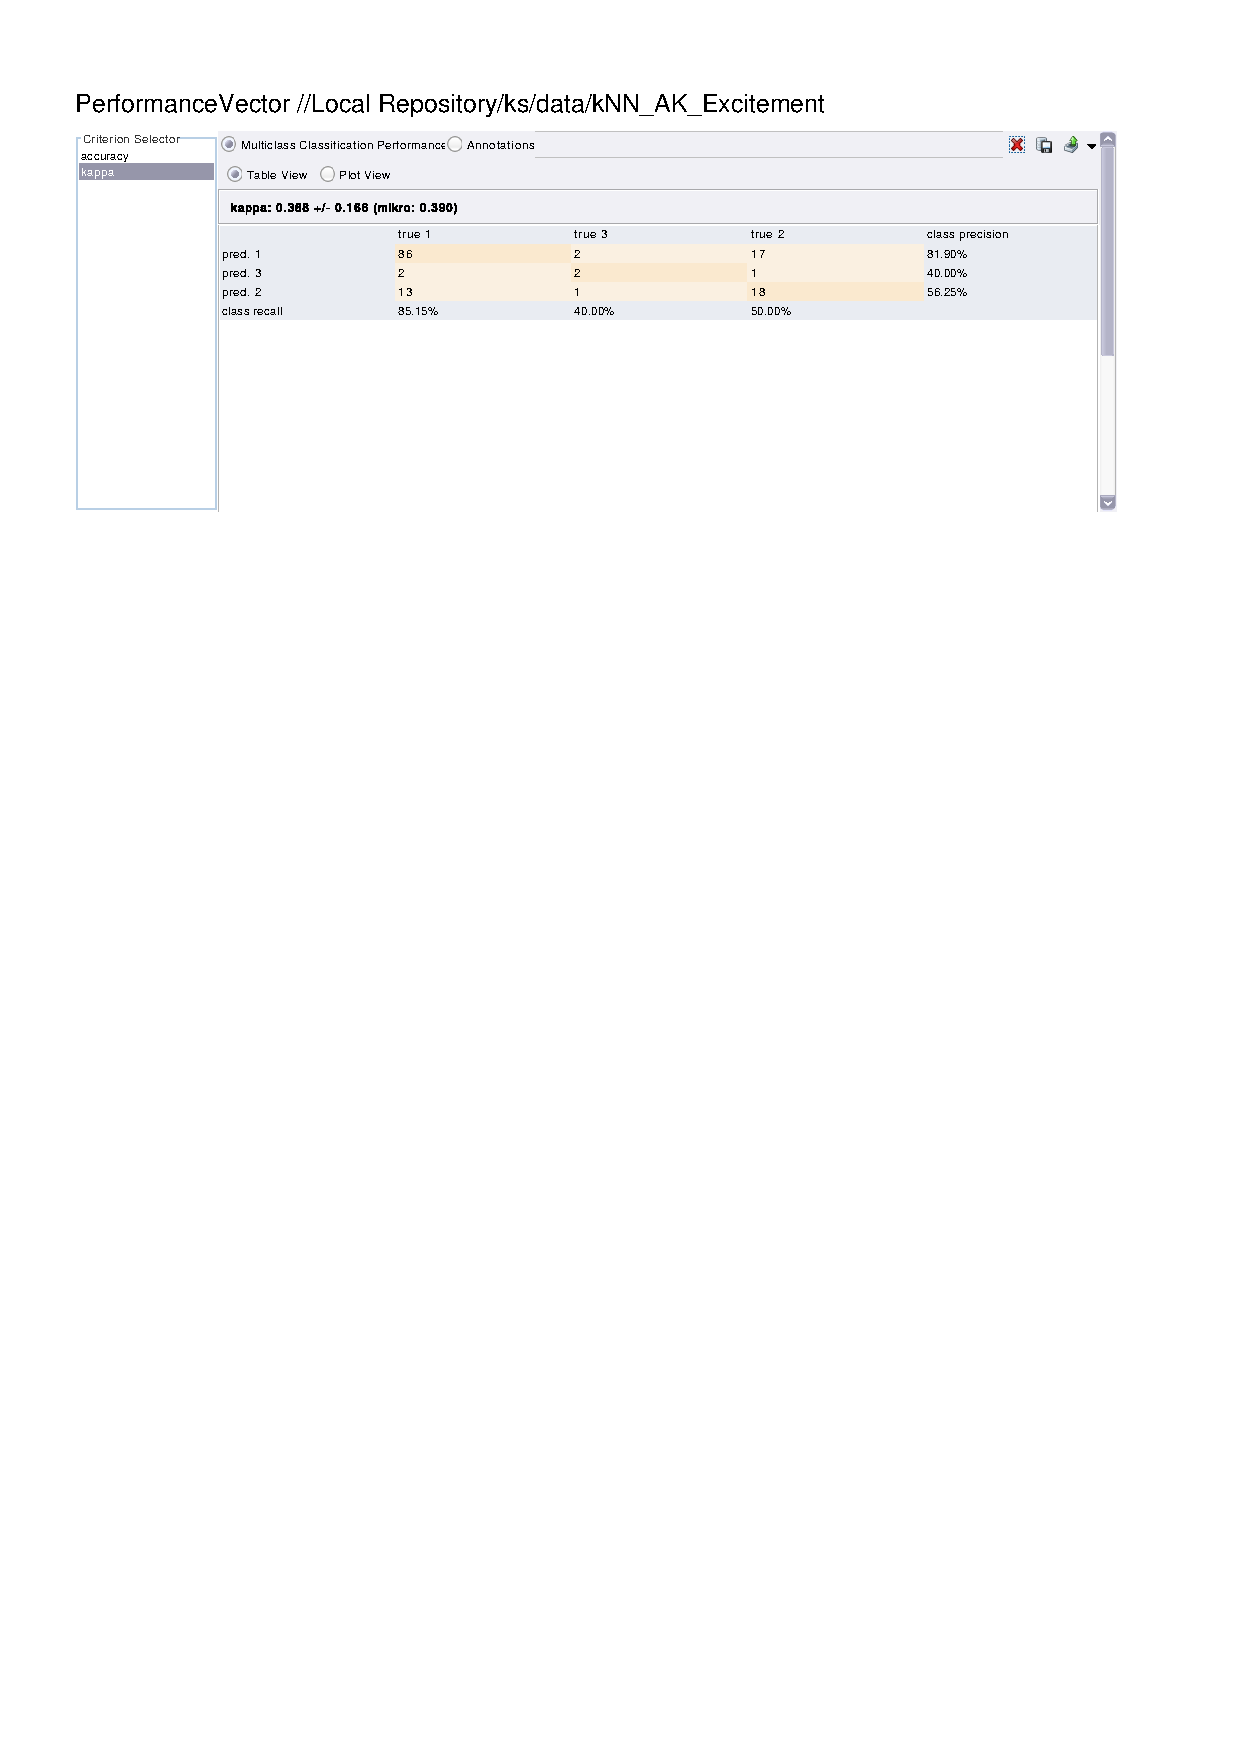
\includegraphics[trim=0 680 0 60,clip,width=16.09cm]{results/kNN_K_Excitement.pdf}} \caption{
} \label{kNN_K_Excitement}
\end{figure}

\clearpage
\FloatBarrier
\subsection{Concentración}
% kNN Focus

\begin{figure}[htp]
  \centerline{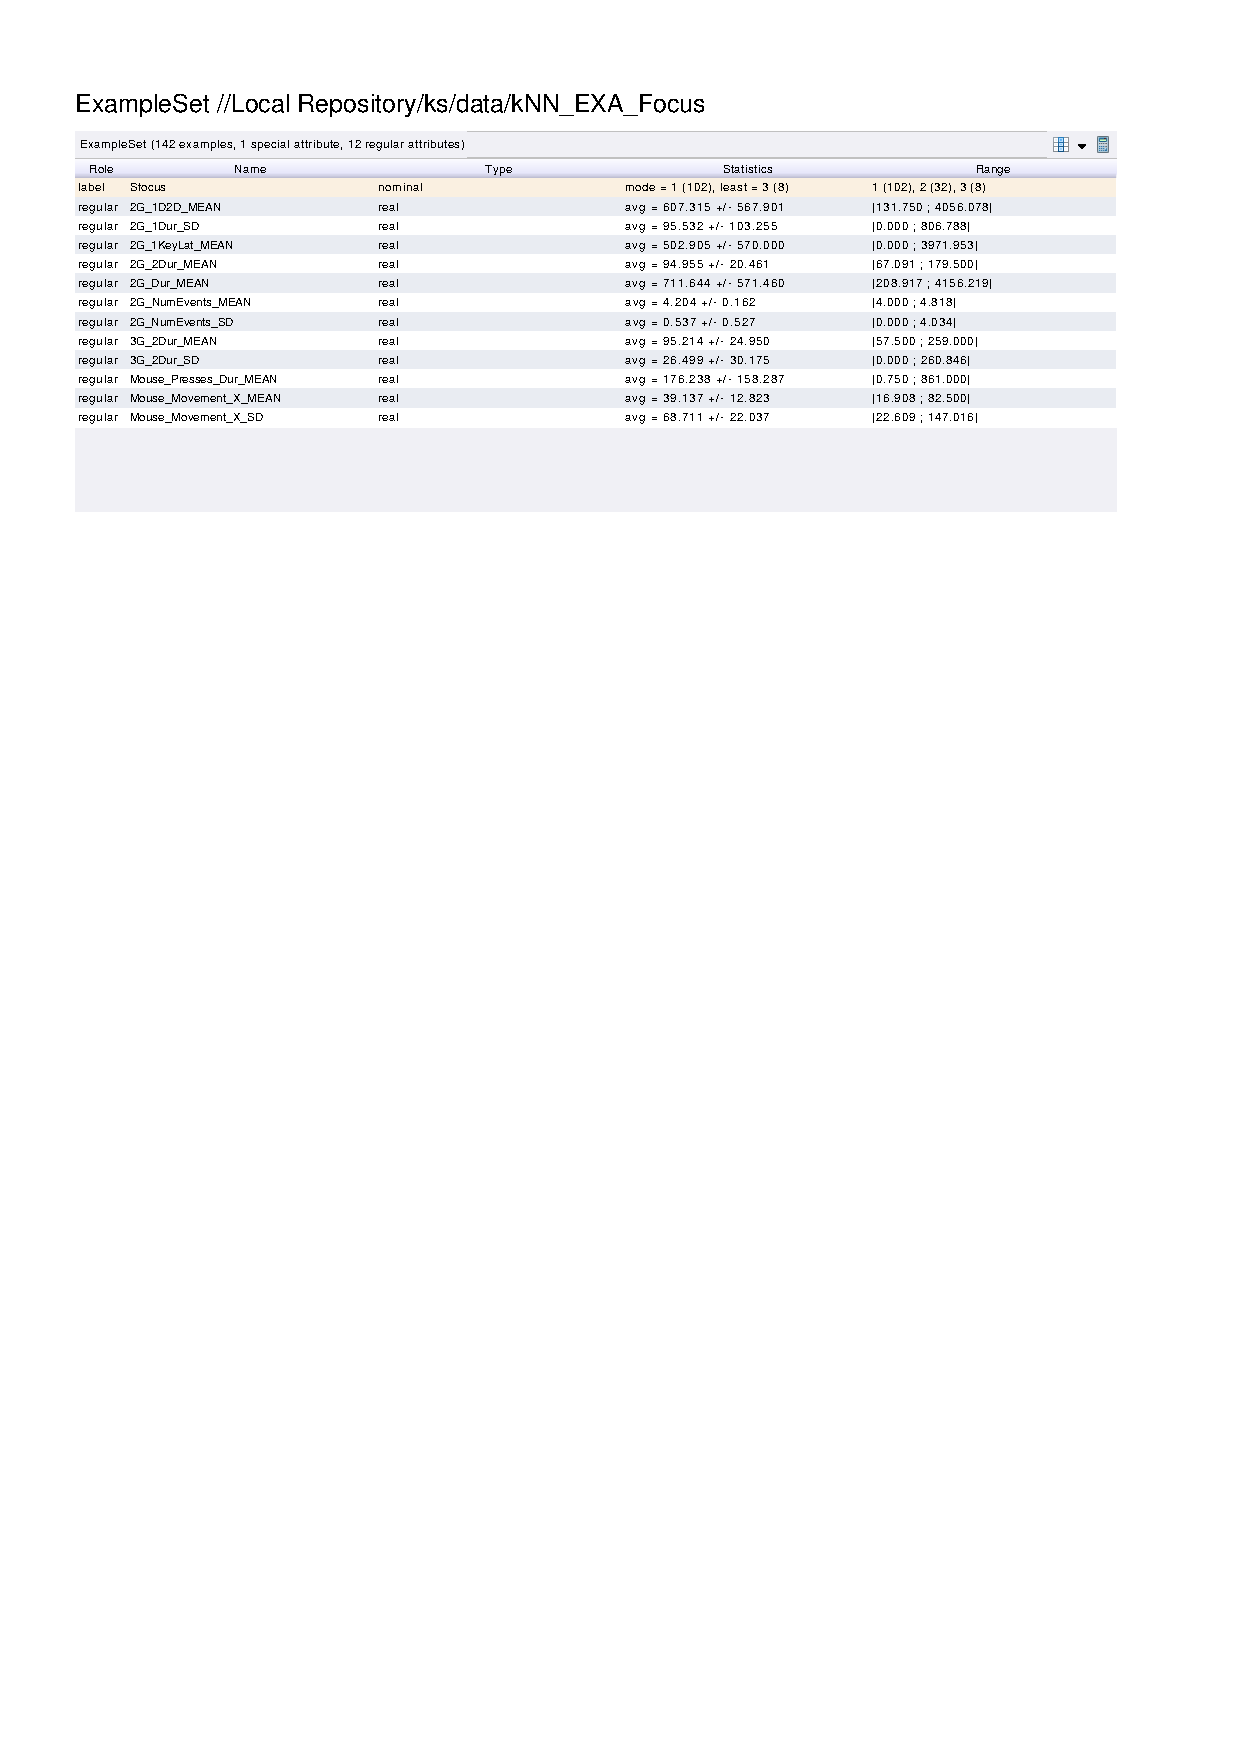
\includegraphics[trim=0 620 0 60,clip,width=16.09cm]{results/kNN_EXA_Focus.pdf}} \caption{
} \label{kNN_K_Focus}
\end{figure}

\begin{figure}[htp]
  \centerline{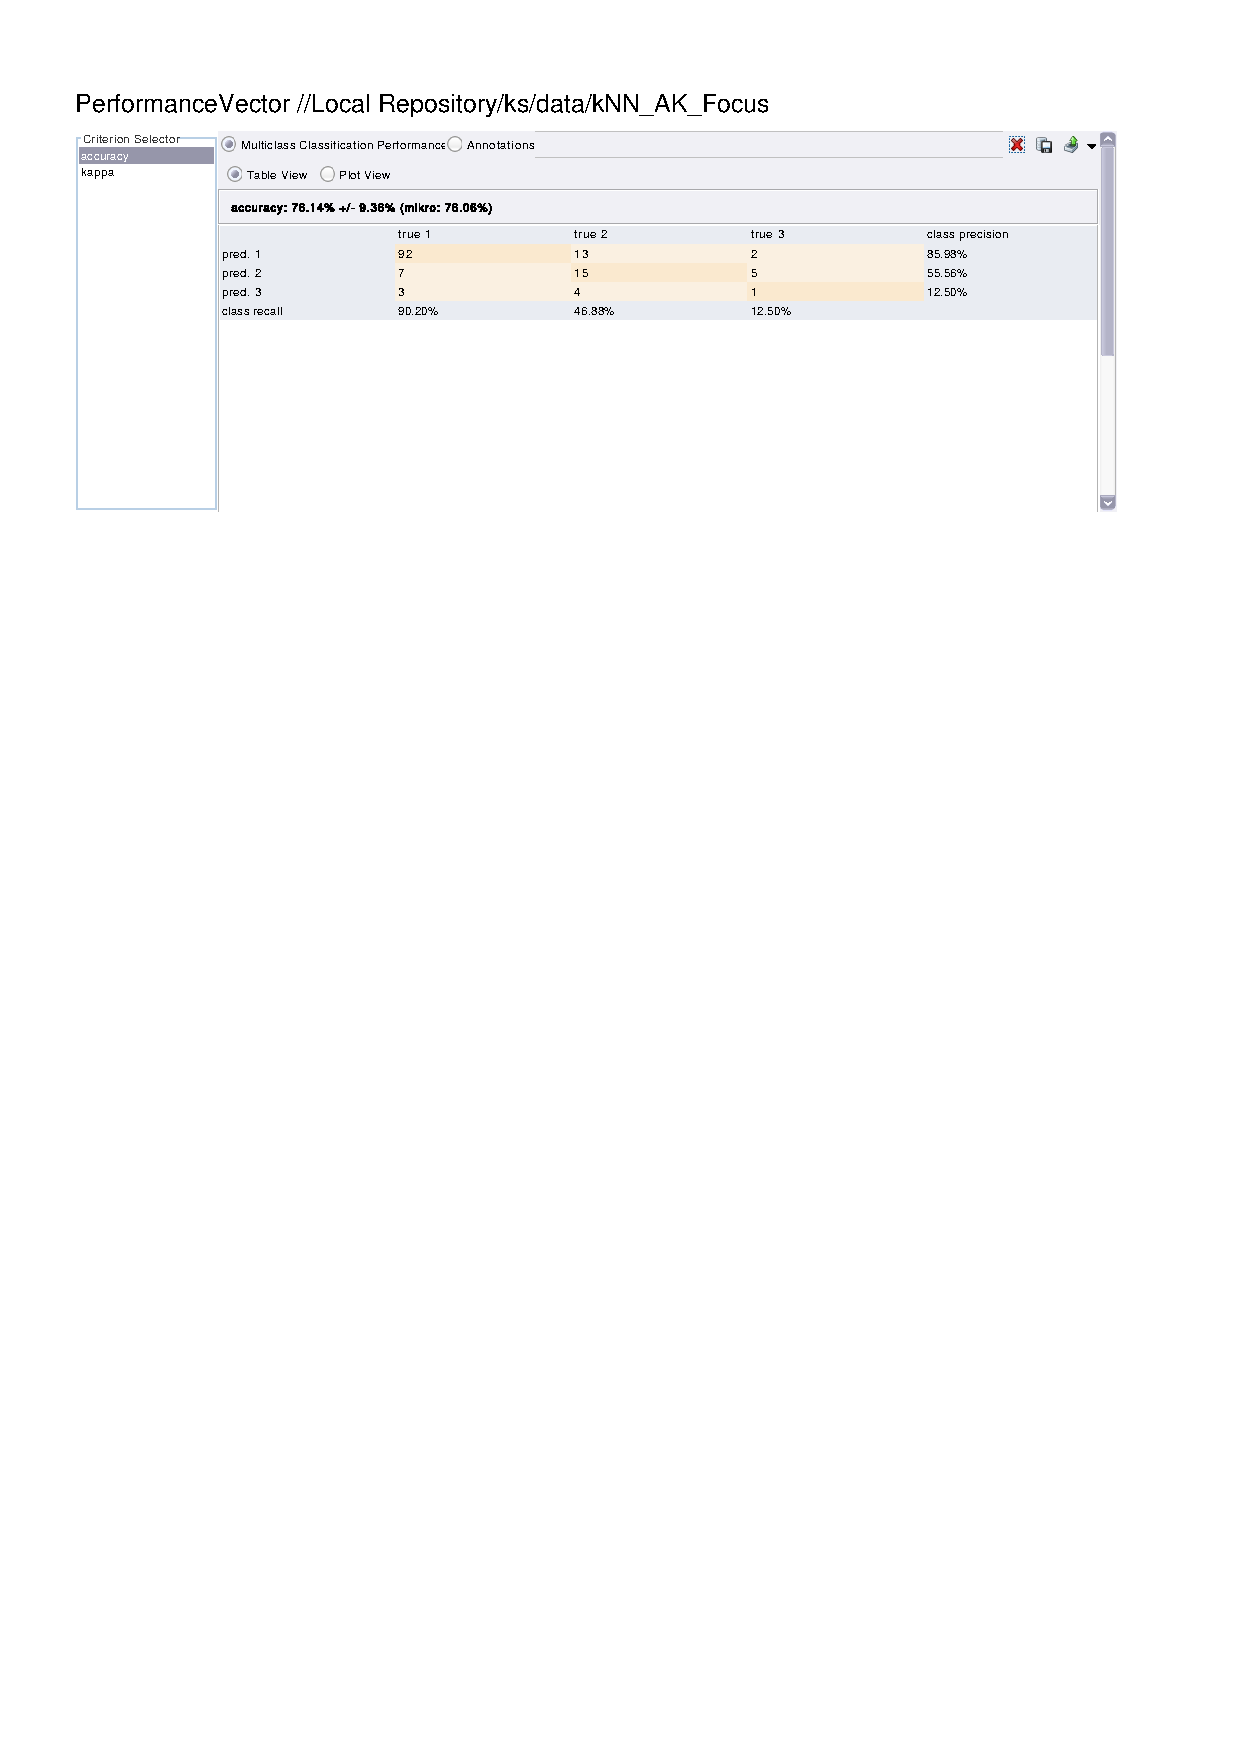
\includegraphics[trim=0 680 0 60,clip,width=16.09cm]{results/kNN_A_Focus.pdf}} \caption{
} \label{kNN_K_Focus}
\end{figure}

\begin{figure}[htp]
  \centerline{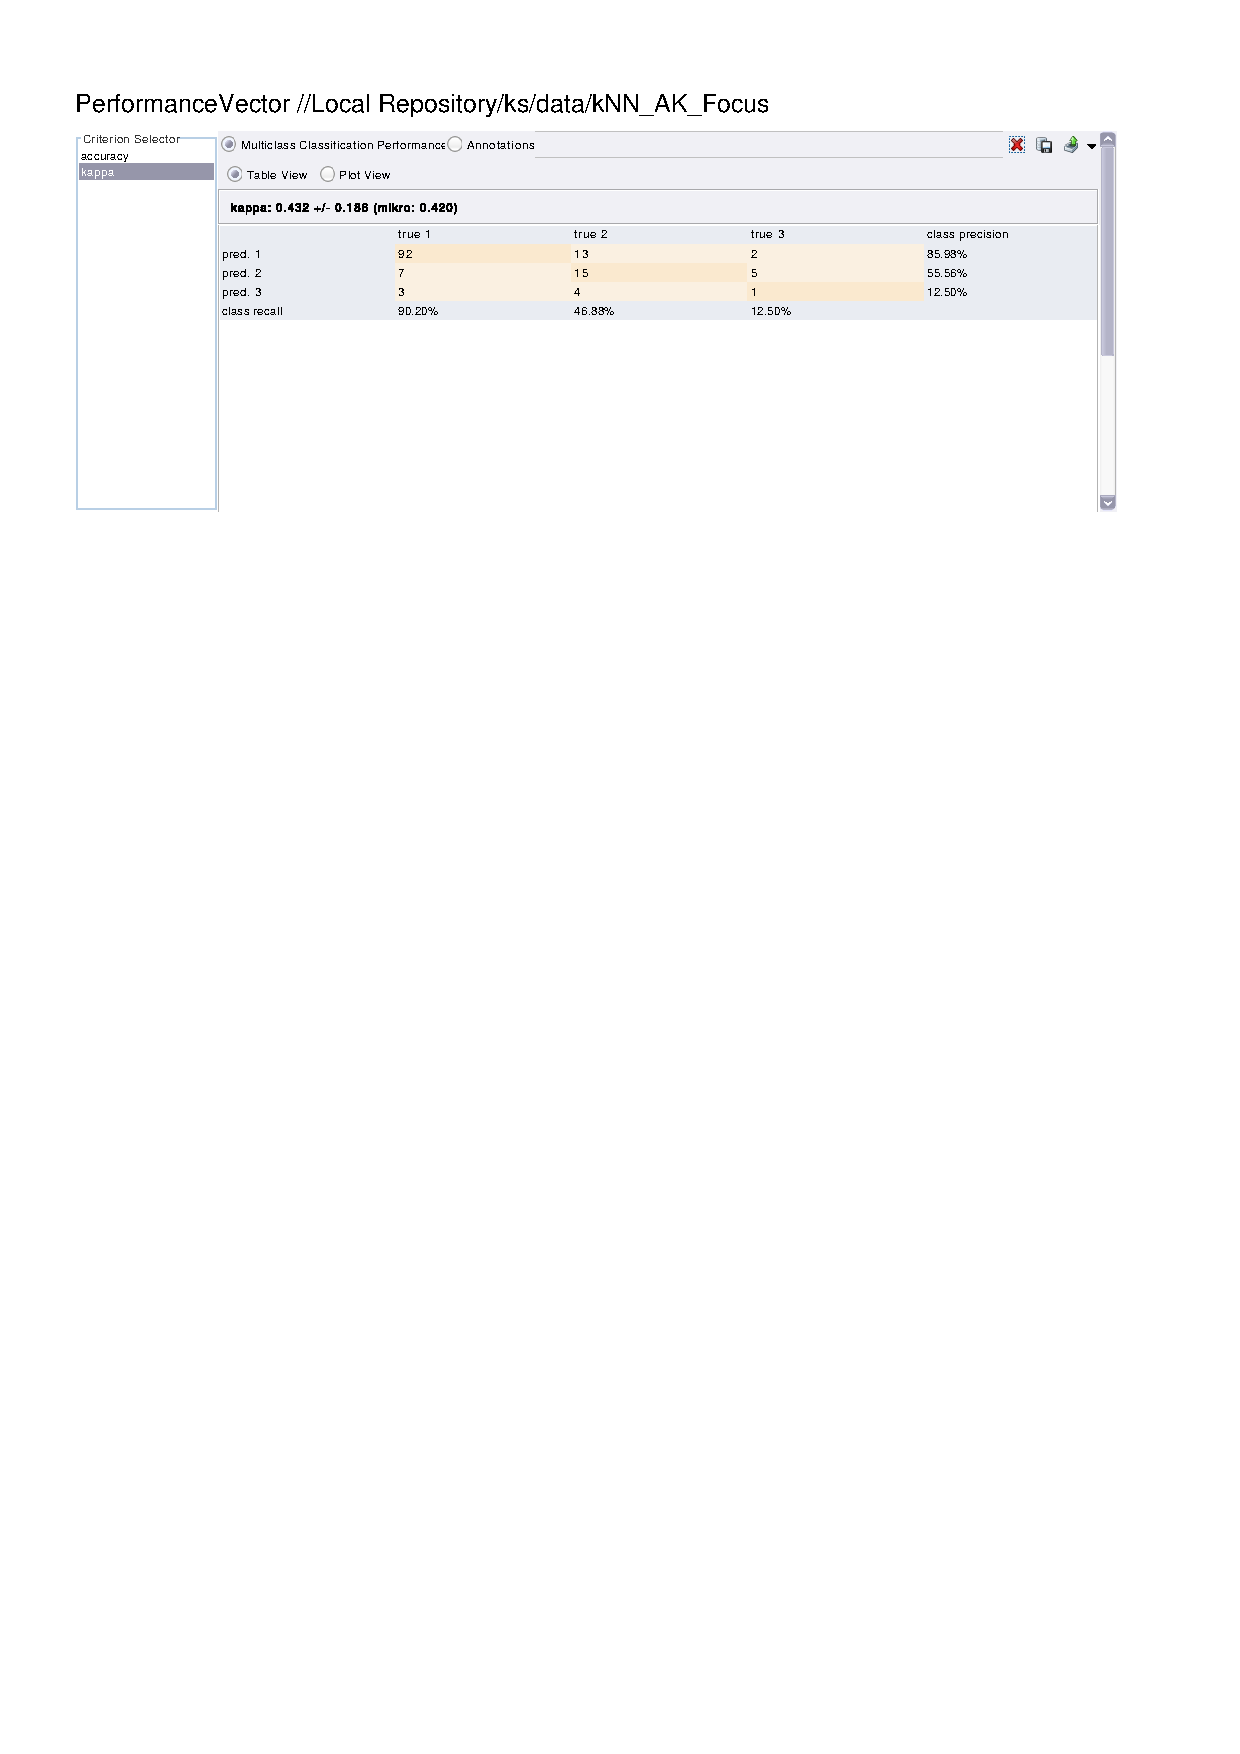
\includegraphics[trim=0 680 0 60,clip,width=16.09cm]{results/kNN_K_Focus.pdf}} \caption{
} \label{kNN_K_Focus}
\end{figure}

\clearpage
\FloatBarrier
\subsection{Frustración}
% kNN Frustration

\begin{figure}[htp]
  \centerline{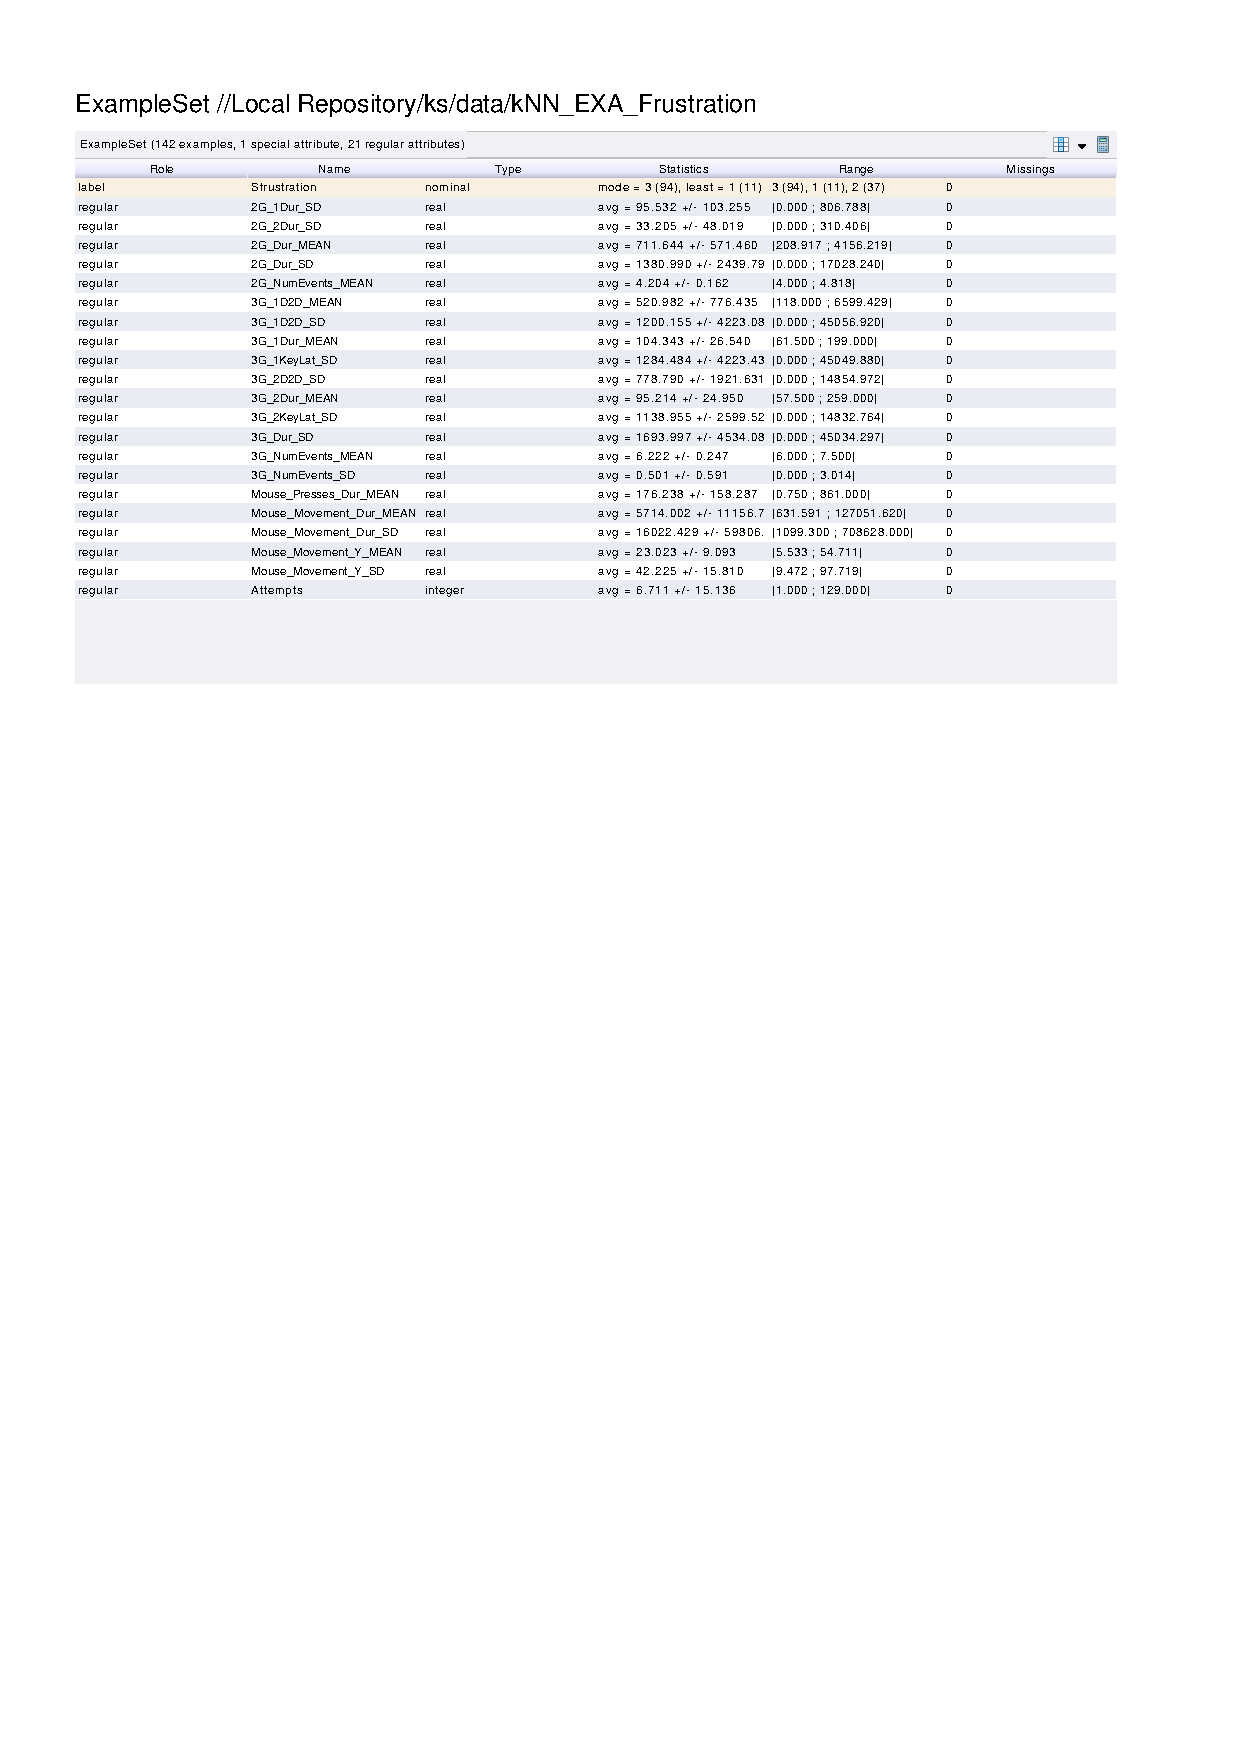
\includegraphics[trim=0 555 0 60,clip,width=16.09cm]{results/kNN_EXA_Frustration.pdf}} \caption{
} \label{kNN_K_Frustration}
\end{figure}

\begin{figure}[htp]
  \centerline{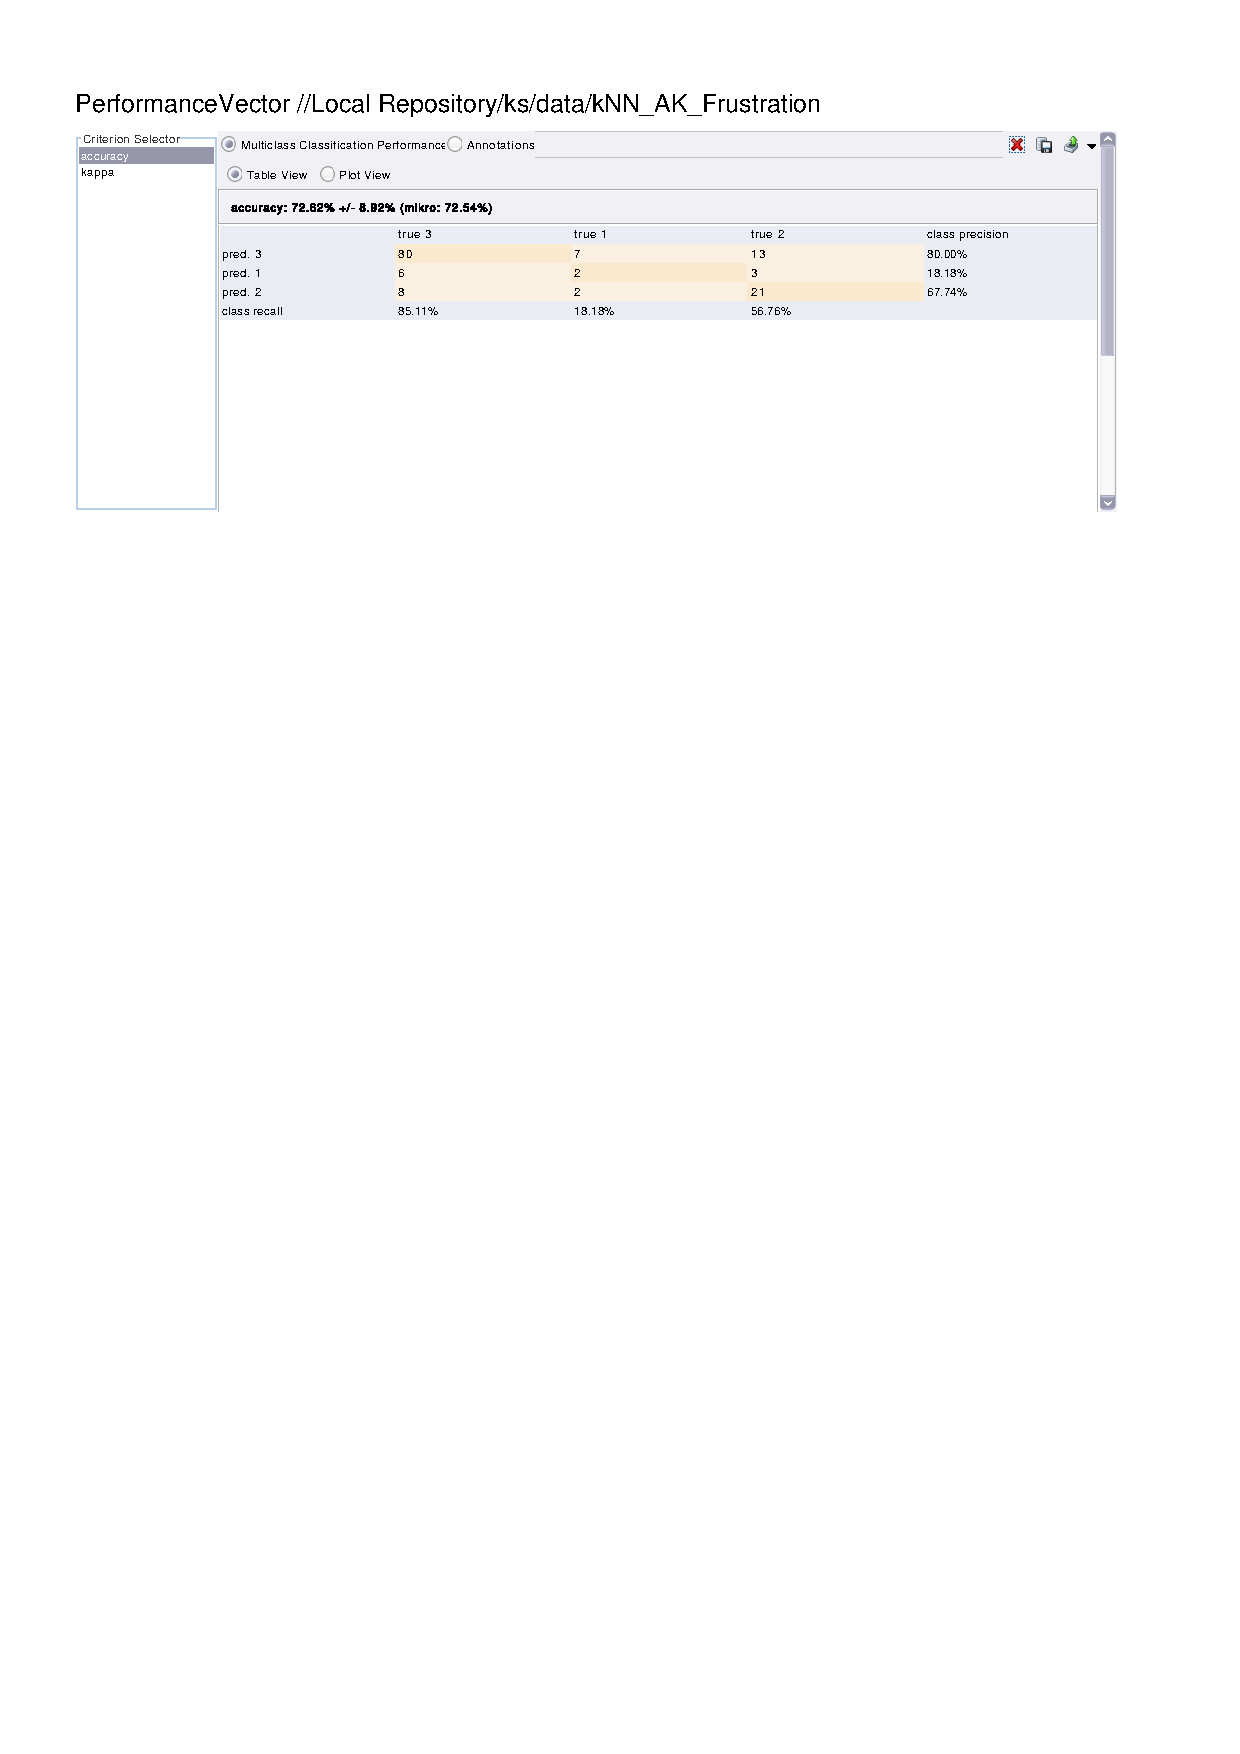
\includegraphics[trim=0 685 0 60,clip,width=16.09cm]{results/kNN_A_Frustration.pdf}} \caption{
} \label{kNN_K_Frustration}
\end{figure}

\begin{figure}[htp]
  \centerline{\includegraphics[trim=0 685 0 60,clip,width=16.09cm]{results/kNN_K_Frustration.pdf}} \caption{
} \label{kNN_K_Frustration}
\end{figure}

\clearpage
\FloatBarrier
\subsection{Relajamiento}
% kNN Relaxation

\begin{figure}[htp]
  \centerline{\includegraphics[trim=0 600 0 60,clip,width=16.09cm]{results/kNN_EXA_Relaxation.pdf}} \caption{
} \label{kNN_K_Relaxation}
\end{figure}

\begin{figure}[htp]
  \centerline{\includegraphics[trim=0 680 0 60,clip,width=16.09cm]{results/kNN_A_Relaxation.pdf}} \caption{
} \label{kNN_K_Relaxation}
\end{figure}

\begin{figure}[htp]
  \centerline{\includegraphics[trim=0 680 0 60,clip,width=16.09cm]{results/kNN_K_Relaxation.pdf}} \caption{
} \label{kNN_K_Relaxation}
\end{figure}

\clearpage
\FloatBarrier
\subsection{Redes Neuronales Artificiales}
\subsection{Aburrimiento}

% ANN Boredom

\begin{figure}[htp]
  \centerline{\includegraphics[trim=0 535 0 60,clip,width=16.09cm]{results/ANN_EXA_Boredom.pdf}} \caption{
} \label{ANN_EXA_Boredom}
\end{figure}

\begin{figure}[htp]
  \centerline{\includegraphics[trim=0 680 0 80,clip,width=16.09cm]{results/ANN_A_Boredom.pdf}} \caption{
} \label{ANN_A_Boredom}
\end{figure}

\begin{figure}[htp]
  \centerline{\includegraphics[trim=0 680 0 80,clip,width=16.09cm]{results/ANN_K_Boredom.pdf}} \caption{
} \label{ANN_K_Boredom}
\end{figure}

\clearpage
\FloatBarrier
\subsection{Distracción}
% ANN Distraction

\begin{figure}[htp]
  \centerline{\includegraphics[trim=0 590 0 60,clip,width=16.09cm]{results/ANN_EXA_Distraction.pdf}} \caption{
} \label{ANN_EXA_Distraction}
\end{figure}

\begin{figure}[htp]
  \centerline{\includegraphics[trim=0 680 0 80,clip,width=16.09cm]{results/ANN_A_Distraction.pdf}} \caption{
} \label{ANN_A_Distraction}
\end{figure}

\begin{figure}[htp]
  \centerline{\includegraphics[trim=0 680 0 80,clip,width=16.09cm]{results/ANN_K_Distraction.pdf}} \caption{
} \label{ANN_K_Distraction}
\end{figure}

\clearpage
\FloatBarrier
\subsection{Entusiasmo}
% ANN Excitement

\begin{figure}[htp]
  \centerline{\includegraphics[trim=0 570 0 60,clip,width=16.09cm]{results/ANN_EXA_Excitement.pdf}} \caption{
} \label{ANN_EXA_Excitement}
\end{figure}

\begin{figure}[htp]
  \centerline{\includegraphics[trim=0 680 0 80,clip,width=16.09cm]{results/ANN_A_Excitement.pdf}} \caption{
} \label{ANN_A_Excitement}
\end{figure}

\begin{figure}[htp]
  \centerline{\includegraphics[trim=0 680 0 80,clip,width=16.09cm]{results/ANN_K_Excitement.pdf}} \caption{
} \label{ANN_K_Excitement}
\end{figure}

\clearpage
\FloatBarrier
\subsection{Concentración}
% ANN Focus

\begin{figure}[htp]
  \centerline{\includegraphics[trim=0 530 0 60,clip,width=16.09cm]{results/ANN_EXA_Focus.pdf}} \caption{
} \label{ANN_K_Focus}
\end{figure}

\begin{figure}[htp]
  \centerline{\includegraphics[trim=0 680 0 80,clip,width=16.09cm]{results/ANN_A_Focus.pdf}} \caption{
} \label{ANN_K_Focus}
\end{figure}

\begin{figure}[htp]
  \centerline{\includegraphics[trim=0 680 0 80,clip,width=16.09cm]{results/ANN_K_Focus.pdf}} \caption{
} \label{ANN_K_Focus}
\end{figure}

\clearpage
\FloatBarrier
\subsection{Frustración}
% ANN Frustration

\begin{figure}[htp]
  \centerline{\includegraphics[trim=0 620 0 60,clip,width=16.09cm]{results/ANN_EXA_Frustration.pdf}} \caption{
} \label{ANN_K_Frustration}
\end{figure}

\begin{figure}[htp]
  \centerline{\includegraphics[trim=0 680 0 80,clip,width=16.09cm]{results/ANN_A_Frustration.pdf}} \caption{
} \label{ANN_K_Frustration}
\end{figure}

\begin{figure}[htp]
  \centerline{\includegraphics[trim=0 680 0 80,clip,width=16.09cm]{results/ANN_K_Frustration.pdf}} \caption{
} \label{ANN_K_Frustration}
\end{figure}

\clearpage
\FloatBarrier
\subsection{Relajamiento}
% ANN Relaxation

\begin{figure}[htp]
  \centerline{\includegraphics[trim=0 600 0 60,clip,width=16.09cm]{results/ANN_EXA_Relaxation.pdf}} \caption{
} \label{ANN_K_Relaxation}
\end{figure}

\begin{figure}[htp]
  \centerline{\includegraphics[trim=0 680 0 80,clip,width=16.09cm]{results/ANN_A_Relaxation.pdf}} \caption{
} \label{ANN_K_Relaxation}
\end{figure}

\begin{figure}[htp]
  \centerline{\includegraphics[trim=0 680 0 80,clip,width=16.09cm]{results/ANN_K_Relaxation.pdf}} \caption{
} \label{ANN_K_Relaxation}
\end{figure}

\clearpage
\FloatBarrier